\documentclass[UTF8,a4paper,12pt]{ctexart}

%---preamble---
%dependency package
\usepackage{amsmath}
\usepackage{amssymb}
\usepackage[colorlinks=false]{hyperref}
\usepackage{setspace}
\usepackage{enumerate}
\usepackage{cases}
\usepackage{tikz}
\usepackage{tikz-3dplot}
\usepackage{caption}
\usepackage{subcaption}
\usepackage{lmodern}
\usepackage{siunitx}
\usepackage[T1]{fontenc}
\usepackage[parfill]{parskip}
\usepackage[toc, page]{appendix} 
\usepackage{color}
\usepackage[most]{tcolorbox}
\usepackage{etoolbox}
\usepackage[intoc]{nomencl}
\usepackage{booktabs}
\usepackage{subcaption}
\usepackage{xcolor} % 支持颜色


%\newcommand{\myfront}{\textbf{\texfsf{Fancy Text}}}

\pagenumbering{arabic} % 阿拉伯数字(默认)
\title{Awakenlion controller}
\author{林梓聪}
\date{\today}
\pagestyle{plain}



%正文区(文稿区)
\begin{document}
%---Style Setting---
\ctexset { 
    section={
     titleformat=\raggedright,
     name=\S
     },
     subsection={
     titleformat=\raggedright
     },
     subsubsection={
     titleformat=\raggedright
     }
}
\newtcolorbox{notitlebox}[2][]
     {
    colback=blue!5!white,colframe=blue!75!black,breakable
    }
\newtcolorbox{titlebox}[2][]
    {
    colback=green!6!white,colframe=green!65!black,
     fonttitle=\bfseries,coltitle=white,                            colbacktitle=green!65!black,
        title=#2,#1,attach boxed title to top center={yshift=-2mm},enhanced,breakable
     }
\linespread{1.35}
\setstretch{1.523}

\definecolor{keil-bg}{RGB}{255, 255, 255}
\definecolor{keil-text}{RGB}{0, 0, 0}
\definecolor{keil-keyword}{RGB}{86, 156, 214}
\definecolor{keil-comment}{RGB}{87, 166, 74}
\definecolor{keil-string}{RGB}{214, 157, 133}
\lstset{
    backgroundcolor=\color{keil-bg},      % 背景色
    basicstyle=\ttfamily\color{keil-text},% 基本字体样式
    keywordstyle=\color{keil-keyword},    % 关键词颜色
    commentstyle=\it\color{keil-comment}, % 注释颜色
    stringstyle=\color{keil-string},      % 字符串颜色
    % numbers=right,                      % 行号在右侧
    numberstyle=\tiny\color{gray},        % 行号样式
    tabsize=4,                             % 制表符宽 
    literate= {\\}{{\textbackslash}}1   % 自动转义       
              {_}{\_}1,                 % 下划线        
      language=C
}
  \maketitle

  % \begin{titlebox}{什么是系统?}

  % \end{titlebox}

%------------------------------------

%----------流程框图------------------
% \tikzstyle{startstop} = [rectangle, rounded corners, minimum width=3cm, minimum height=1cm,text centered, draw=black, fill=red!30]
% \tikzstyle{process} = [rectangle, minimum width=3cm, minimum height=1cm, text centered, draw=black, fill=orange!30]
% \tikzstyle{decision} = [diamond, minimum width=3cm, minimum height=1cm, text centered, draw=black, fill=yellow!30]
% \tikzstyle{arrow} = [thick,->,>=stealth]


\tikzstyle{startstop} = [  minimum width=2.5cm, minimum height=0.8cm,text centered]
\tikzstyle{process} = [ minimum width=2.5cm, minimum height=0.8cm, text centered,]
\tikzstyle{sys} = [rectangle, minimum width=2.5cm, minimum height=0.8cm, text centered, draw=black]
\tikzstyle{arrow} = [thick,->,>=stealth]







  \begin{center}
    \tableofcontents
  \end{center}
  \newpage

  \section{引言}
  \begin{flushleft}
    \hspace{2em}此文档的初衷是让大家轻松地入门电控代码的控制器,缩短大家从理论到实践的时间。文档将会结合信号与系统和自动控制原理的相关知识,为大家讲解我们战队所需要的控制器,以及如何设计控制器。如果觉得作者本人写的不够详细或者有失偏颇,本人会在每一个知识点的后面附带上我学习过的网址,大家可以搜索着来学习。
    \par\hspace{2em}本文档还会手把手教你如何操作,即使不看理论知识也可以按照步骤来直接得到结果。


  \end{flushleft}
  \section{理论知识}

  \begin{flushleft}
    以下是设计一个控制器所需要用到的理论知识,知识深度仅停留在工程应用的层面,不需要深究其数学原理,但是想要看懂还是需要基本的高数知识。以下的知识只需要将他们看作工具就好了,我们最终的目的就是得到传递函数,依据传递函数来设计所需要的控制器。我尽量会以是什么,怎么用的框架来解释下面的知识,其更深层的含义我会附上链接。
  \end{flushleft}

  \subsection{线性时不变系统(LTI)}
    \begin{flushleft}
      为什么我们要先讲线性时不变系统呢?因为我们战队的代码所设计和分析的控制器都是基于线性时不变系统来研究的。
      \par 实际上线性时不变系统是一个理想化的数学模型,在生活中基本不存在完全符合线性时不变系统定义的系统。主要是以下两个原因:
      \begin{notitlebox}
          \par1.线性系统的限制:
          \begin{itemize} 
            \item 许多系统在小信号范围内表现出线性特性,但在大信号条件下会出现非线性失真,如放大器在信号过强时的饱和现象。
            \item 机械系统如弹簧-质量系统在小振幅下可近似为线性,但超过弹性限度时会表现出非线性行为
          \end{itemize}

          \par2.时不变性的挑战:
          \begin{itemize} 
          \item 理想的时不变系统要求其参数不随时间变化,但在现实中,环境因素如温度、湿度可能影响系统参数,导致时变性。
          \item 电子元件可能因老化或温度变化而改变特性,从而引入时变性。  
          \end{itemize}
          \begin{flushleft}
           但因为LTI模型简单易于处理,其分析方法(如傅里叶变换、拉普拉斯变换、卷积等)是通用的,所以我们会在一定合理的范围和时间内,将系统近似为LTI系统。\par 即使是遇到完全是非线性和时不变的系统我们都会尽量将其线性化(如工作点线性化、分段近似等)和时不变近似(如慢变参数近似、时间平均化等),以此来简化我们的分析。
          \end{flushleft}
      \end{notitlebox}
    \end{flushleft}
    \begin{flushleft}
      OK,了解完上面的原因后,我们来真正的开始学线性时不变系统。
    \end{flushleft}
    \subsubsection{系统}
    \begin{titlebox}{什么是系统?}
      \begin{flushleft}
        
        \par 系统是指若干关联的事物组合而成具有特定功能的整体,系统可以是我们的云台,可以是一个电机,也可以是一个底盘。
        \par 系统的作用: 对输入信号进行加工和处理,将其转换为输出信号
        \par 表示如下:
        \begin{tikzpicture}[node distance=4.5cm]
          
          \node (start) [startstop] {输入信号(激励)};
          \node(input)[sys,right of=start]{系统};
          \node (output) [process, right of=input, xshift=0cm] {输出信号(响应)};
          \draw [arrow] (start) -- (input);
          \draw [arrow] (input) -- (output);
        \end{tikzpicture}

        \par 下面请记住这个重要的概念,
        \par 动态系统:系统的响应不仅与激励有关{$f_{(\cdot)}$}而且和过去的状态{$x_{(0)}$}有关。含有记忆元件(电容、电感等)的系统就是动态系统。
        \begin{itemize} 
          \item $y_{(\cdot)}$完全响应:零状态响应+零输入响应
          \item $y_{zs}{(\cdot)}$零状态响应:系统在初始时刻没有储能,所有响应均由输入信号引起。
          \item  $y_{zi}{(\cdot)}$零输入响应:零输入响应完全由系统的初始状态决定,与输入信号无关。(如在电路系统中,电容一开始就储存了能量,这个时候即使没有输入信号也会有对应的响应,就像高中学的LC震荡电路一样)
        \end{itemize}
     
    \end{flushleft}
 
  \end{titlebox}


\begin{flushleft}
  
\end{flushleft}
    
\subsubsection{线性系统}
  \begin{titlebox}{什么是线性系统}
    \begin{flushleft}
      线性系统的充要条件为系统同时满足可加性和其次性 
    
      1、齐次性
      \par
      \begin{tikzpicture}[node distance=5cm]
        \node (start) [startstop] {$f_1$};
        \node(input)[sys,right of=start]{线性系统};
        \node (output) [process, right of=input, xshift=0cm] {$y_1$};
        \draw [arrow] (start) -- (input);
        \draw [arrow] (input) -- (output);
      \end{tikzpicture}
        \par
        \begin{tikzpicture}[node distance=5cm]
          \node (start) [startstop] {$a\cdot f_1$};
          \node(input1)[sys,right of=start]{线性系统};
          \node (output) [process, right of=input1, xshift=0cm] {$a \cdot y_1$};
          \draw [arrow] (start) -- (input1);
          \draw [arrow] (input1) -- (output);
        \end{tikzpicture}
        思考一下:如果一个系统为$y=ax+b$那么它是不是线性系统呢?\\
        2、可加性
        \par
        \begin{tikzpicture}[node distance=5cm]
          \node (start) [startstop] {$f_1$};
          \node(input)[sys,right of=start]{线性系统};
          \node (output) [process, right of=input, xshift=0cm] {$y_1$};
          \draw [arrow] (start) -- (input);
          \draw [arrow] (input) -- (output);
        \end{tikzpicture}
          \par
          \begin{tikzpicture}[node distance=5cm]
            \node (start) [startstop] {$f_2$};
            \node(input1)[sys,right of=start]{线性系统};
            \node (output) [process, right of=input1, xshift=0cm] {$y_2$};
            \draw [arrow] (start) -- (input1);
            \draw [arrow] (input1) -- (output);
          \end{tikzpicture}
          \begin{tikzpicture}[node distance=5cm]
            \node (start) [startstop] {$f_1+f_2$};
            \node(input1)[sys,right of=start]{线性系统};
            \node (output) [process, right of=input1, xshift=0cm] {$y_1+y_2$};
            \draw [arrow] (start) -- (input1);
            \draw [arrow] (input1) -- (output); 
          \end{tikzpicture}
          \par {\scriptsize 注:$f_1$为激励,$y_1$为响应,且线性系统都为同一个系统}
  
    \end{flushleft}
    
  \end{titlebox}
  \subsubsection{时不变系统}
    \begin{titlebox}{什么是时不变系统}
      \begin{flushleft}
        简单来说就是$f_{(t)}$延迟多少,$y_{(t)}$就延迟多少
      \end{flushleft}
      \begin{flushleft}
        \begin{tikzpicture}[node distance=5cm]
          \node (start) [startstop] {$f_{(t)}$};
          \node(input1)[sys,right of=start]{线性系统};
          \node (output) [process, right of=input1, xshift=0cm] {$y_{(t)}$};
          \draw [arrow] (start) -- (input1);
          \draw [arrow] (input1) -- (output); 
        \end{tikzpicture}

        \begin{tikzpicture}[node distance=5cm]
          \node (start) [startstop] {$f_{(t-t_0)}$};
          \node(input1)[sys,right of=start]{线性系统};
          \node (output) [process, right of=input1, xshift=0cm] {$y_{(t-t_0)}$};
          \draw [arrow] (start) -- (input1);
          \draw [arrow] (input1) -- (output); 
        \end{tikzpicture}
        \par {\scriptsize 注:$f_{(t)}$为激励,$y_{(t)}$为响应,且线性系统都为同一个系统}
        \par 如何判断一个系统是不是时不变呢,我们可以设一个延时激励,带入系统得到一个响应,然后再对原来响应延时,判断两者是否相等,稍微给个题目大家看看:
        \begin{center}
           \par 例:判断系统是否是时不变系统$y(t-t_0)=tf(t)$
           令$g(t)=f(t-t_d)$,$T[in]$为激励信号输入后系统的响应
           \begin{equation}
            T[g(t)] = t\cdot g(t)=t\cdot g(t-t_d)
            \end{equation}
            \begin{equation}
              y(t-t_d)= (t-t_d) \cdot f(t-t_d)
              \end{equation}
          \begin{flushleft}
              对比(1)、(2)式可得出,(1)式是延时激励,(2)式是原本的系统响应延迟,两式不相等,所以该系统不是时不变系统。  
          \end{flushleft}
           
        \end{center}
       
      \end{flushleft}
    \end{titlebox}
    
    \subsubsection{线性时不变系统(LTI)}
    \begin{titlebox}{什么是LTI呢}
      显而易见,一个系统同时满足是线性和时不变性就是LTI系统了
            $$ \text{LTI系统分析方法}
            \begin{cases}
             \text{输入输出法(外部法)}\\
             \text{状态变量法(内部法)}
            \end{cases}$$
          
            $$ \text{外部法}
            \begin{cases}
             \text{时域分析(微分方程)}\\
              \text{变换域法}
                $$ 
                \begin{cases}
                  \text{连续系统}
                  $$ 
                  \begin{cases}
                    \text{频域法(傅里叶变换)}\\
                    \text{复频域法(拉普拉斯变换)}
                  \end{cases}$$
                  \\
                  \text{离散系统———频域法(离散傅里叶变换)、Z域法}
                \end{cases}$$
            \end{cases}$$
    \end{titlebox}
    \par {\scriptsize 注:本文主要讲解外部分析法,内部法涉及现代控制理论可以自行了解}
  

  \subsection{微分方程}
  \begin{flushleft}
    了解了什么是线性时不变系统后,现在我教你们怎么在时域上分析连续的系统,这里我只会教公式解法而不会特别具体,因为等我们学习到了频域之后,我们基本上都会用频域的知识去分析系统
  \end{flushleft}
  \begin{titlebox}{微分方程的经典解法}
    这下面的系统方程可以理解为这是我们分析系统的物理特性(系统建模)所列出来的方程
    \par $y^{(n)}_{(t)}+a_{n-1} \cdot y^{(n-1)}_{(t)}+...+a_{1} \cdot y^{(1)}_{(t)}+a_{0} \cdot y{(t)}$
  \par $=b_m \cdot f^{(m)}_{(t)}+b_{m-1} \cdot f^{(m-1)}_{(t)}+...+b_{1} \cdot f^{(1)}_{(t)}+b_{0} \cdot f{(t)}$
    \par  {\scriptsize 注:$y^{(n)}_{(t)}$为y的n阶导}
    \par 最后我们要求的是:
    \par
      $y(t)\text{(完全解)} =y_h(t)\text{(齐次解)}+y_p(t) \text{(特解)}$

  \begin{flushleft}
    \vspace{1cm} 
    ①先求齐次解:$y^{(n)}_{(t)}+a_{n-1} \cdot y^{(n-1)}_{(t)}+...+a_{1} \cdot y^{(1)}_{(t)}+a_{0} \cdot y{(t)}=0$ 
    \par 齐次解的特征根为:$\lambda^n+a_{n-1} \cdot \lambda^{n-1}+...+a_1 \cdot \lambda+a_0=0$ 
  
    \begin{tabular}{cc}
      \toprule
      特征根 $\lambda$ & 齐次解 $y_h(t)$ \\
      \midrule
      单实根 & ${Ce^{\lambda t}}$\\
      2重根 & $\left( C_1t+C_0 \right) e^{\lambda t}$ \\
      一对共轭复根$\lambda_{1,2}=\alpha \pm j\beta $ 
      & 
      $e^{\alpha t}\left[ C\ \cos \left( \beta t \right) +D\sin \left( \beta t \right) \right]$ \\
      \bottomrule
    \end{tabular}
    \par ②再求特解:
  \end{flushleft}
    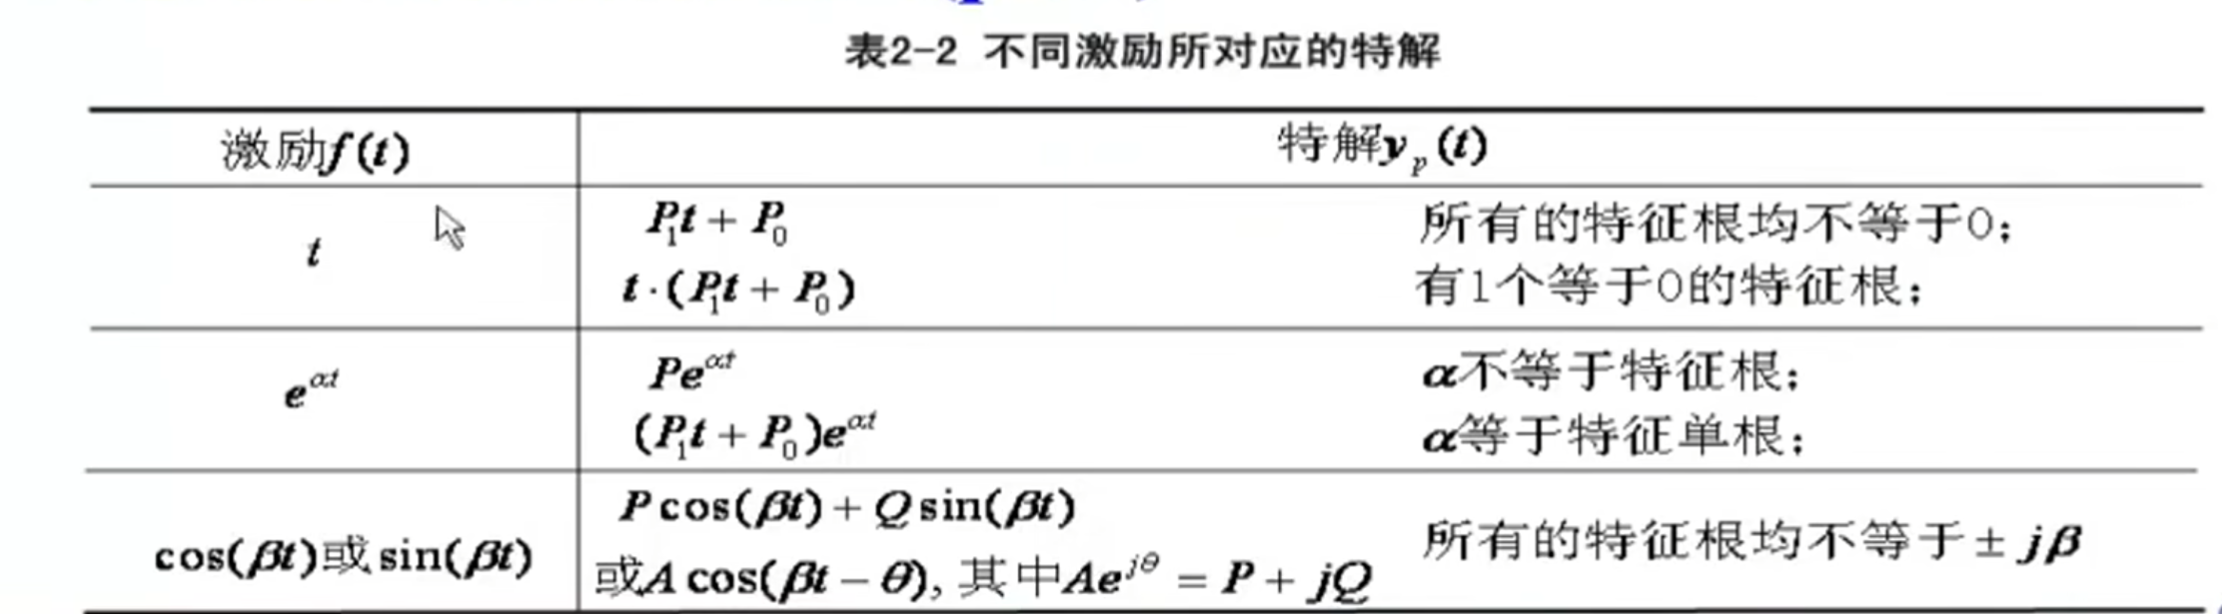
\includegraphics[width=12.5cm]{picture/a_differential_equation.png}
 
  \end{titlebox}

  \begin{flushleft}
    看完上面的东西之后大家可能蒙蒙的,接下来我会完整地分析一个经典的二阶系统————弹簧质量阻尼系统 
  \end{flushleft}
  
   
    \begin{notitlebox}
     
          \includegraphics[width=10cm]{picture/spring_damper.png}
      \par 再看看最后计算的结果
      \par 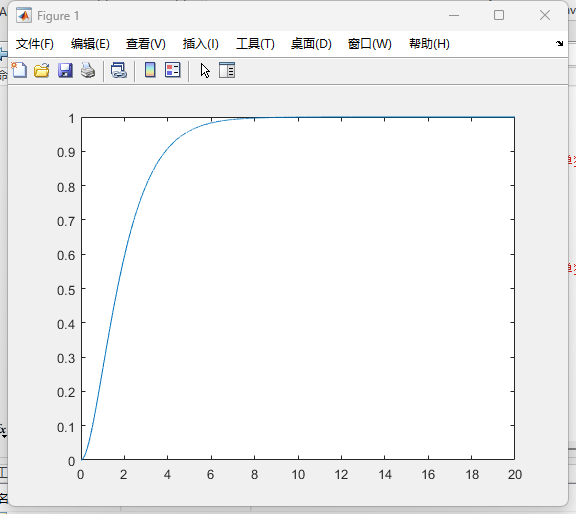
\includegraphics[width=10cm]{picture/result.png}
   \par 从图像看出,用恒定1N的力去推物块,他会在9s左右到达1m处,然后到达二力平衡,一直停在1m处,
   \par 建议大家试试在此系统上用不同的系数(改变b、m、k),不同的输入看看得到的结果是什么,自己算一遍会有不一样的收获。
    \end{notitlebox}
    \begin{flushleft}
      在现实生活中不一样的系统需要对应的系统建模方法,比如电路系统需要用KCL、KVL等,热力学需要PV=nRT、卡诺循环等。这些在你们需要的时候可以自行去探索,这里就不过多赘述了
    \end{flushleft}
  \subsection{卷积}
     \subsubsection{基本信号及其响应}
     \begin{flushleft}
      在讲卷积之前,我需要引入两个基本信号,以此来推导卷积的公式,同时这两个基本信号也非常重要,大家一定要熟悉。
     \end{flushleft}
     \begin{titlebox}{阶跃函数}
   
   $$ \varepsilon \left( t \right)=
      \begin{cases}
       0 \text{\hspace{0.5cm},t<0}\\
       1 \text{\hspace{0.5cm},t>0}
      \end{cases}$$
      \begin{center}
        \par 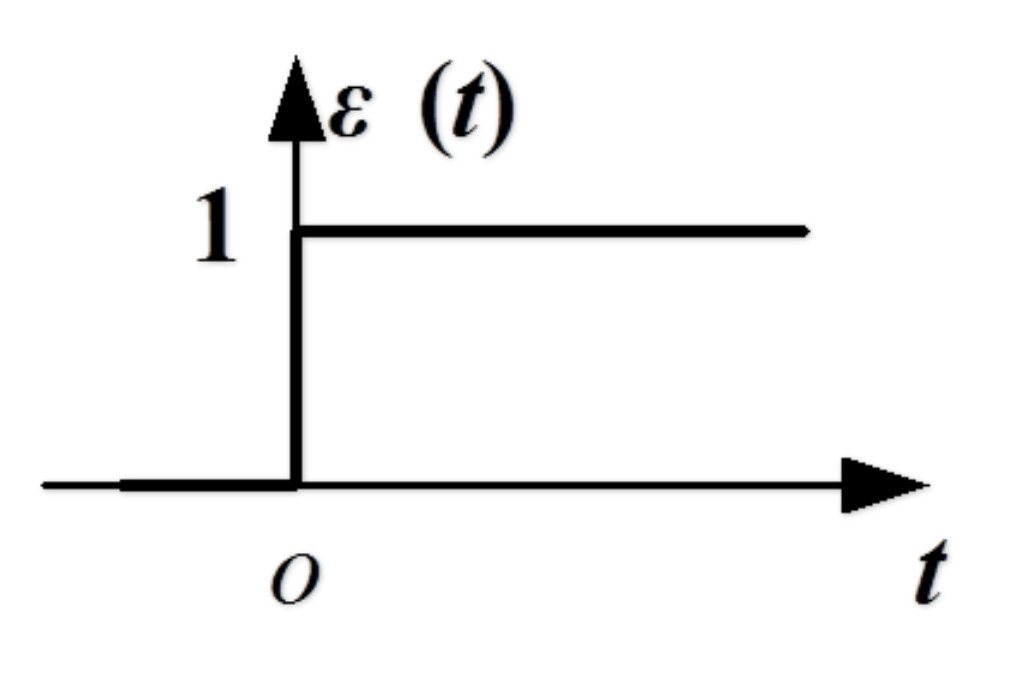
\includegraphics[width=6cm]{picture/step_signal.png}
      \end{center}
      阶跃函数是物理系统无法实现的,我们稍微想想就知道了,在生活中什么数值的上升下降都有一个过程比如温度:从1~100℃,在你对水加热的过程中,水肯定是每一个温度都会经历,而不是直接从1到100的直接跳变。
     \end{titlebox}

    \begin{titlebox}{冲激函数}
      
      $$\varepsilon'(t)= \delta \left( t \right)=
      \begin{cases}
       0 \text{\hspace{0.5cm},$t\ne 0$}\\
       \int_{-\infty }^{+\infty } \delta(t) \, dt=1
      \end{cases}$$
      \begin{center}
        \par 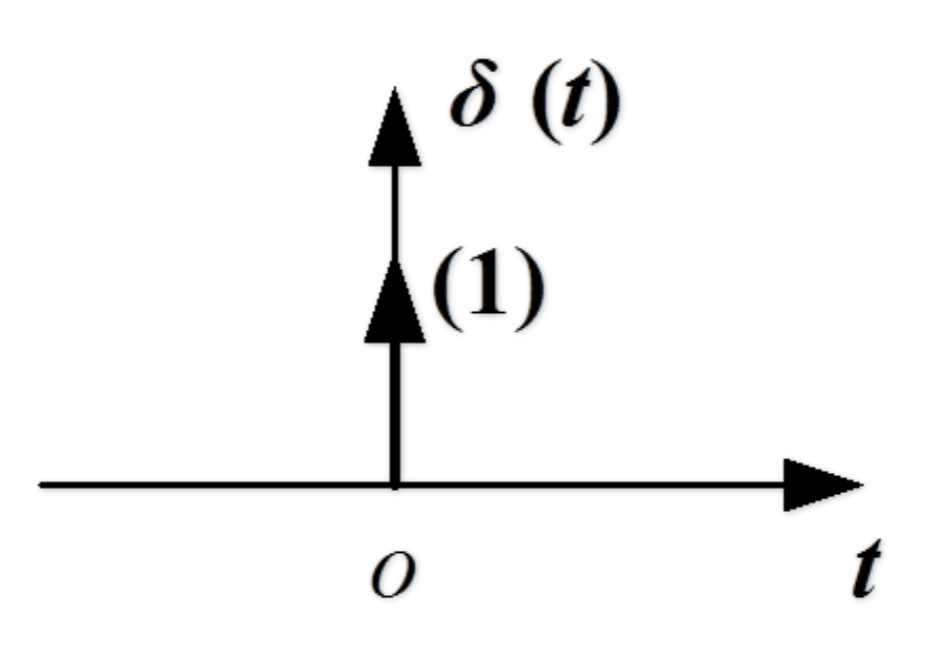
\includegraphics[width=6cm]{picture/deta_signal.png}
      \end{center}
      \begin{flushleft}
        $\delta(t)$ 是我们人为定义的一个函数,他是由$ \varepsilon (t)$求导可得。
        \par 可以理解为在$\delta(t)$冲激函数可以理解为一个在t=0 处无限高、无限窄,但面积为 1 的脉冲
      \end{flushleft}
       \par \textbf{冲激函数的性质:}
       \begin{itemize} 
        \item 取样性质: $\int_{-\infty }^{+\infty } \delta(t)\varphi(t)  \, dx=\varphi(0) $ {\scriptsize 可以自己想想为什么}  
        \item 缩放性:$\delta (at) =\dfrac{1}{|a|}  \delta ( t ) $
        \item 奇偶性:$\delta ( t )=\delta ( -t ) $ (偶函数)
        
      \end{itemize}
    \end{titlebox}
      
  \begin{flushleft}
    \begin{titlebox}{基本信号的响应}
      就一个很简单的例子,我上面所分析的弹簧质量阻尼系统,我的输入就是一个阶跃信号,而得到的响应就是我们分析求的$y(t)$,也就是\textbf{阶跃响应}。\\
      那如果我们想给一个冲激信号呢?你可以想象我们踢这个物块一脚,这一脚的力度很大,且脚和物块接触的时间无限短、趋近于0,那么你的输入就接近于一个冲激信号,你们可以尝试输入一个冲激信号看一看能不能求出来他的\textbf{冲激响应}(求的时候记住$\varepsilon'(t)= \delta \left( t \right)$)
    \end{titlebox}
    \subsubsection{卷积的理解}
    \begin{titlebox}{什么是卷积}
      卷积的本质:信号的分解。\\
      拿我们上面的弹簧阻尼质量系统来举例,假设我们现在的输入信号如下的黑色曲线,然后我们简单的把其离散化(此时我们只看那3个矩形波,不需要看曲线)
      \begin{center}
        \par 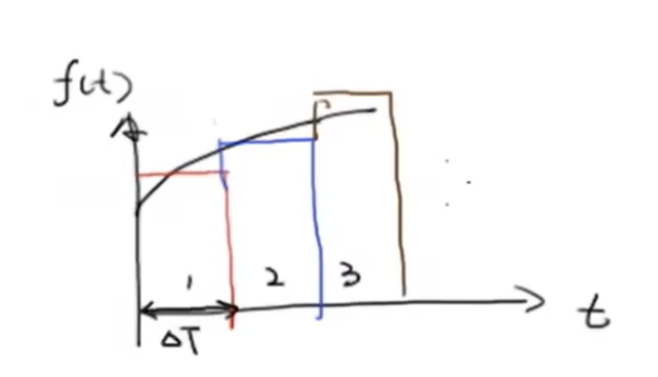
\includegraphics[width=6cm]{picture/juanji_1.png}
      \end{center}
      然后,我们假设只输入第一个矩形波的响应如下:
      \begin{center}
        \par 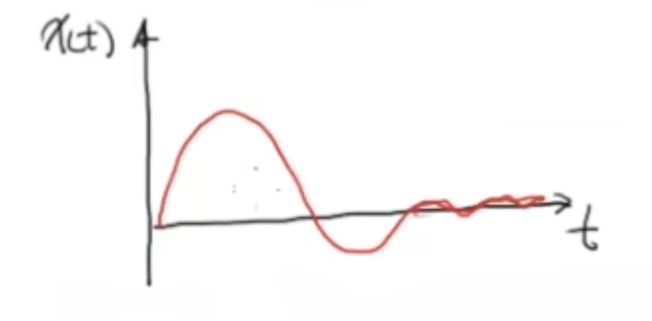
\includegraphics[width=6cm]{picture/juanji_2.png}
      \end{center}
      那么根据LTI系统的齐次性和时不变性,我们将三个输入信号看作单独作用于这个系统,我们可以得到以下的三个单独的响应
      \begin{center}
        \par 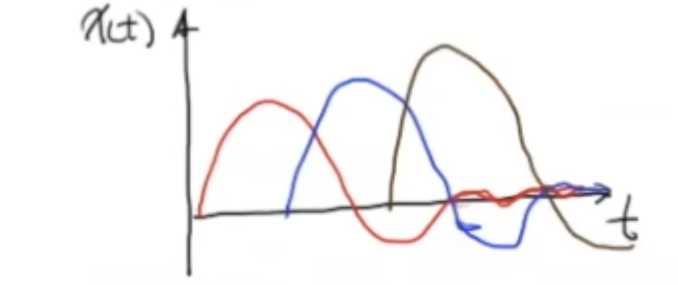
\includegraphics[width=6cm]{picture/juanji_3.png}
      \end{center}
      知道了三个信号单独作用的响应后,我们试着将他们一起作用在这个弹簧阻尼系统上(这里的“一起”不是说同时作用的意思,而是说,利用LTI系统的可加性,对t时刻之前的输入响应进行求和)。如下图,在画线的那个时间点我们的响应是三个单独信号在t时刻的叠加,所以$x(t)=\varSigma$ {\scriptsize (系统对t时刻前输入响应的和)}。
      \begin{center}
        \par 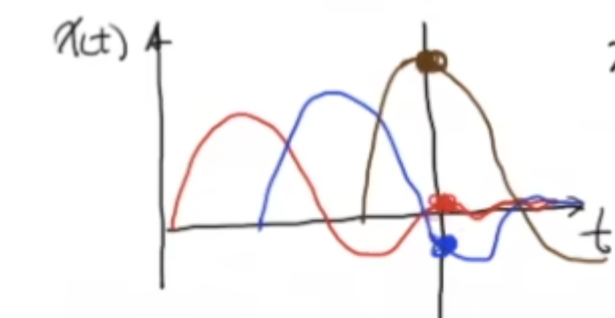
\includegraphics[width=6cm]{picture/juanji_5.png}
      \end{center}
      试想一下,如果我们将$\varDelta T$趋近于0,那么我们离散的矩形波就变成了一条直线且有无数条,而且重新接近回我们的曲线,此时我们的求和就成了积分(函数的面积),为了实现这一目的我们先将输入信号先单位化,就是将矩形波化简为下面这个$\delta _{\varDelta}(t)$ 函数的A倍:\\{\scriptsize 思考一下当$\varDelta T$趋近于0,这个函数是什么函数}
      \begin{center}
        \par 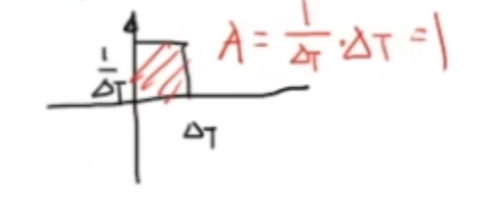
\includegraphics[width=6cm]{picture/juanji_6.png}
      \end{center}

      看下面左图,对于输入信号为,我们的响应是$h _{\varDelta}(t)$,那么由LTI的性质我们可以推出第二和第三条式子(其实就是把前三幅图用公式给你们描述一遍,大家可以翻前去看看)\\
      这里的A是代表矩形波的面积(看右图,底×高),也表示 \( A \) 个单位的 \(\delta_{\varDelta}(t)\)。把 \( A = \varDelta T f(i\varDelta T) \) 带入式三,最后得式四:
        \begin{tabular}{cc}
            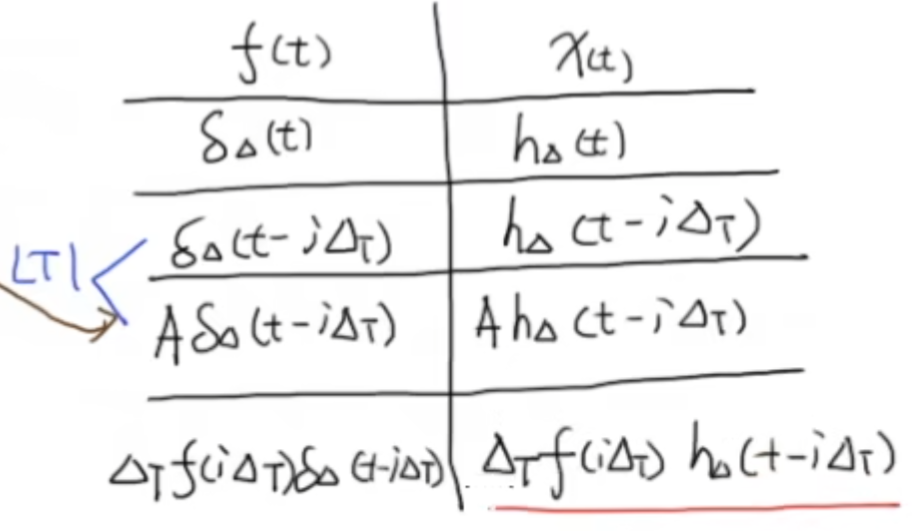
\includegraphics[width=0.45\textwidth]{picture/juanji_8.png} &
            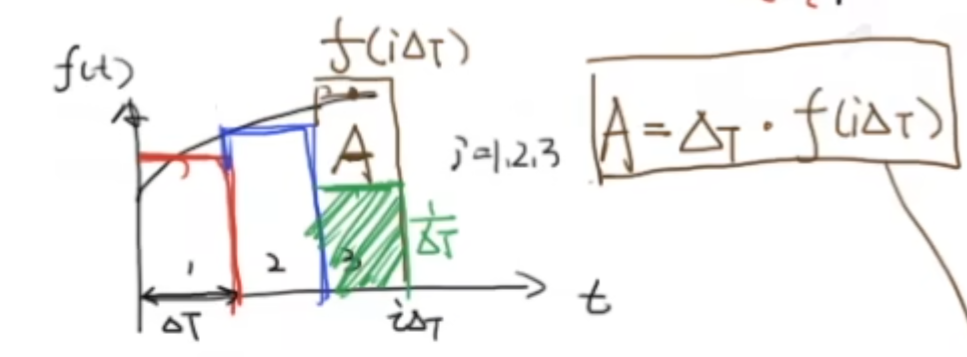
\includegraphics[width=0.45\textwidth]{picture/juanji_7.png} \\
        \end{tabular}
        \begin{flushleft}
          \vspace{1cm}
          上面说过,求t时刻的响应就是将t时刻之前的输入响应进行求和:
          \\$t=i\varDelta T$时: $x\left( t \right) =\sum_{i=0}^i{\varDelta Tf\left( i\varDelta T \right) \cdot}h_{\varDelta}\left( t-i\varDelta T \right) $,\\
          令$\underset{\varDelta T\rightarrow 0}{\lim}$,$h_{\varDelta}\left( t \right) \rightarrow h\left( t \right)$,$\varDelta T=d\tau$,$i\varDelta T=\tau$,
          \begin{align*}
            x(t) &=\int_0^t{f\left( \tau \right)}h\left( t-\tau \right) d\tau  \\
                 &= f(t)*h(t)
          \end{align*}
          上面的第二条式子就记作$f(t)$和$h(t)$的卷积,$x(t)$则是他们通过卷积运算得出来的一个新函数。
        \end{flushleft}
    
     
    \end{titlebox}
    随便解个密,当$\underset{\varDelta T\rightarrow 0}{\lim}$时,\(\delta_{\varDelta}(t)\rightarrow \delta(t)\),所以h(t)是冲激响应。\textbf{ 由此可以看出对于LTI系统,冲激响应可以完全定义系统(即系统冲激响应等于系统),也就是说只要能得出冲激响应,就可以知道系统长什么样。所以系统的输出等于输入卷积冲激响应(系统本身)}
  \end{flushleft}

    \begin{flushleft}
      \begin{notitlebox}
      \  我们现在得出来了卷积的表达式,我们试试从另外一个角度来看待卷积,仔细观察卷积的表达式$x(t) =\int_0^t{f\left( \tau \right)}h\left( t-\tau \right) d\tau $。
       \\将$f(\tau)$看作一个函数,则$h(\tau)$是先翻转成$h(-\tau)$,然后再平移到t,得到$h(t-\tau)$,并且将从0平移到t这过程中和$f(\tau)$一一对应的乘积进行求和。\\
         所以,我们可以简单的把卷积理解为它将两个函数结合在一起,产生第三个函数。这个新函数可以看作是一个函数在另一个函数上的“滑动窗口”积分。\\
       不懂的话就看下面第一条链接,回来后应该能大致理解我说的是什么意思了
    \end{notitlebox}
   \end{flushleft}
    由于本人对卷积的理解也不算特别深刻,而卷积又是一个很有趣的知识点,所以大家可以看下面链接的视频,加深大家对卷积的理解\\
    \href{https://www.bilibili.com/video/BV1Vd4y1e7pj/?spm_id_from=333.337.search-card.all.click&vd_source=b02f21f21dd17ebeef8dac9338c9d06c}{https://www.bilibili.com/video/BV1Vd4y1e7pj}。\\
    \href{https://www.bilibili.com/video/BV1cs411W74f/?spm_id_from=333.337.search-card.all.click&vd_source=b02f21f21dd17ebeef8dac9338c9d06c}{https://www.bilibili.com/video/BV1cs411W74f}。
  \subsection{拉普拉斯变换}
 \begin{flushleft}
  前面我们运用时域分析对弹簧质量阻尼系统进行了分析,从这一节开始我们就开始运用频域的分析方法来解析系统,而拉普拉斯变换就是经典控制理论中很重要的一个数学工具,可以将时域转换为频域,从而降低分析难度。
 \end{flushleft}
 \subsubsection{频域和傅里叶变换}
  在学习拉普拉斯变换之前,大家需要先对频域有一个基本的认识,并且也简单的了解一下傅里叶变换,傅里叶变换如果想深入学习的话,可以自己查资料学习,傅里叶也是一个很重要的知识点,大家尽量去掌握。
  \begin{titlebox}{什么是频域}
    在我们平常的生活中,我们习惯用时间来描述一件事情,如人的身高体重随时间的变化、上面我们以时间为自变量来描述的弹簧阻尼质量系统等,以时间作为参照来观察动态世界的方法我们称其为时域分析。
    \\现在我们不用时域来分析事情,我们将坐标轴x轴的变量换成频率$\omega$,我们用频率来分析和描述一件事,这就称为我们的频域分析。
  \end{titlebox}
  \begin{flushleft}
    知道了什么是频域,那么我们怎么样才能将时域的东西变成频域呢?这就要用到我下面说的傅里叶变换了
  \end{flushleft}
  \begin{titlebox}{傅里叶变换}
    任何周期函数,都可以看作是不同振幅,不同相位正弦波的叠加。其定义式如下:
    \begin{align*}
      F\left( j\omega \right) =\int_{-\infty}^{\infty}{f\left( t \right)}e^{-j\omega t}dt
    \end{align*}
    傅里叶变换需要$f(t)$满足绝对可积的条件:
    \begin{align*}
      \int_{-\infty}^{\infty}{\left| f\left( t \right) \right|}dt
    \end{align*}
    指数衰减函数,如$f(x)=e^{-x}$;有界函数在有限区间上也绝对可以积,如$f(x)=sin(x)$在$[0,\pi]$上绝对可积;而$f(x)=1$就不是绝对可积的了。这些大家都可以代入到定义式自己验证一下。
  
  \end{titlebox}
    大家可以点下面的链接去更深入的了解傅里叶变换
    \href{https://blog.csdn.net/l494926429/article/details/51818012?ops_request_misc=%257B%2522request%255Fid%2522%253A%25228ab09c60845aafcecfa8aa2ca8e01526%2522%252C%2522scm%2522%253A%252220140713.130102334..%2522%257D&request_id=8ab09c60845aafcecfa8aa2ca8e01526&biz_id=0&utm_medium=distribute.pc_search_result.none-task-blog-2~all~top_positive~default-1-51818012-null-null.142^v101^pc_search_result_base1&utm_term=%E5%82%85%E9%87%8C%E5%8F%B6%E5%8F%98%E6%8D%A2&spm=1018.2226.3001.4187}{深入浅出的讲解傅里叶变换}
  \subsubsection{拉普拉斯变换定义}
  \begin{titlebox}{什么是拉普拉斯变换}
    对一个函数f(t)做拉普拉斯变化,可以将其从时域(t)转换到复数域(s),它的定义为
    \begin{align*}
      \mathcal{L}\left[ f\left( t \right) \right] =F\left( s \right) =\int_0^{\infty}{f\left( t \right)}e^{-st}dt
    \end{align*}
    其中,$s=\sigma +j\omega $,是一个复数
    \\举个例子,$\mathcal{L}[e^{-at}]=\dfrac{1}{s+a}$
   \\ 证:
   \begin{align*}
    \mathcal{L}[e^{-at}] &= \int_0^{\infty}{e^{-at}e^{-st} dt}\\
         &= \int_0^{\infty}{e^{-\left( a+s \right) t}dt}\\
         &= -\dfrac{1}{s+a}e^{-\left( a+s \right) t}\left| _{0}^{\infty} \right. \\
         &=\dfrac{1}{s+a}
  \end{align*}
  
  \end{titlebox}
  基本上,如果你需要进行拉普拉斯变换的话都可以这样直接套公式,大家也可以求一下其他函数的拉普拉斯变换熟悉一下。但是如果每次都需要求的话就会显得十分麻烦,所以给大家一个表,一些基本函数的拉普拉斯变换都在里面,大家要用的时候可以直接查表。
  \subsubsection{常见的拉普拉斯变换公式}
  \begin{titlebox}{1}
    \begin{flushleft}
    \begin{tabular}{c|c|c}
      \toprule
      \hspace{1cm}原函数\hspace{1cm} & \hspace{1cm}拉普拉斯变换\hspace{1cm} & 收敛域(实部 $\sigma$)\\
      \midrule
      $f(t)$ & $F(s) =\mathcal{L}[f(t)]$ &  \\
      \midrule
      $\delta(t)$   &   1   &  $-\infty <\sigma<\infty$\\
      \midrule
      1   &   $\dfrac{1}{s}$   &  $\sigma>0$  \\
      \midrule
      $t^n$   &   $\dfrac{n!}{s^{n+1}}$   &  $\sigma>-a$  \\
      \midrule
      $e^{-at}$   &   $\dfrac{1}{s+a}$   &  $\sigma>-a$  \\
      \midrule
      $sin(at)$   &   $\dfrac{a}{s^2+a^2}$   &  $\sigma>0$  \\
      \midrule
      $cos(-at)$   &   $\dfrac{s}{s^2+a^2}$   &  $\sigma>0$  \\
      \bottomrule
    \end{tabular}
   
  \end{flushleft}
  \end{titlebox}
  \subsubsection{拉普拉斯收敛域}
  看到上面那个表,肯定会有人疑惑收敛域是什么东西,其实上文我们讲傅里叶变换的时候我们也有涉及到一点,我们说过傅里叶变换需要满足这个函数是绝对可积的,而拉普拉斯变换通过引入衰减因子$e^{-\sigma t}$,拓展了其适用性,使原来不满足傅里叶变换条件的信号也能进行变化。
  
  \begin{notitlebox}
   \\我们来举个例子,
   \begin{center}
      $F(S)=\mathcal{L}[e^{-at}] = \int_0^{\infty}{e^{-at}e^{-st} dt}$
   \end{center}
 
   将$s=\sigma +j\omega $代入上式,得
   \begin{center}
      $F(S)=\mathcal{L}[e^{-at}] = \int_0^{\infty}{e^{-(a+\sigma )t} \cdot e^{-j\omega t} dt}$
   \end{center}
   上面式子中的积分是由两部分相乘而得。首先看$e^{-j \omega t}$这一项是一个复数。根据欧拉公式得$e^{-j \omega t}=cos{\omega t} -j sin{\omega t}$,所以随着t的增加在复平面上做顺时针的运动,而他的幅值$|e^{-j \omega t}|$是恒定不变且等于1,如下左图(对于欧拉公式得证明这个大家可以去查资料,或者我记得的话会在文章最后面写一个附录来证明)。所以用它乘以$e^{-(a+\sigma )t}$这一项不会对积分的收敛产生影响。这也可以从另外一个角度看,根据欧拉公式,$e^{-j \omega t}$仅仅是引入了正弦和余弦量(引入振动),而振动又会有正有负,不会在单一方向上增加或减少。因此要满足函数绝对可以积,e的指数部分要小于0,即
   \begin{center}
    $-(a+\sigma)<0$
    \\$\sigma > -a$    
   \end{center}

   所以,$\sigma > -a$ 是$\mathcal{L}[e^{-at}]=\dfrac{1}{s+a}$的收敛域,如下右图
   \\
   \begin{tabular}{cc}
    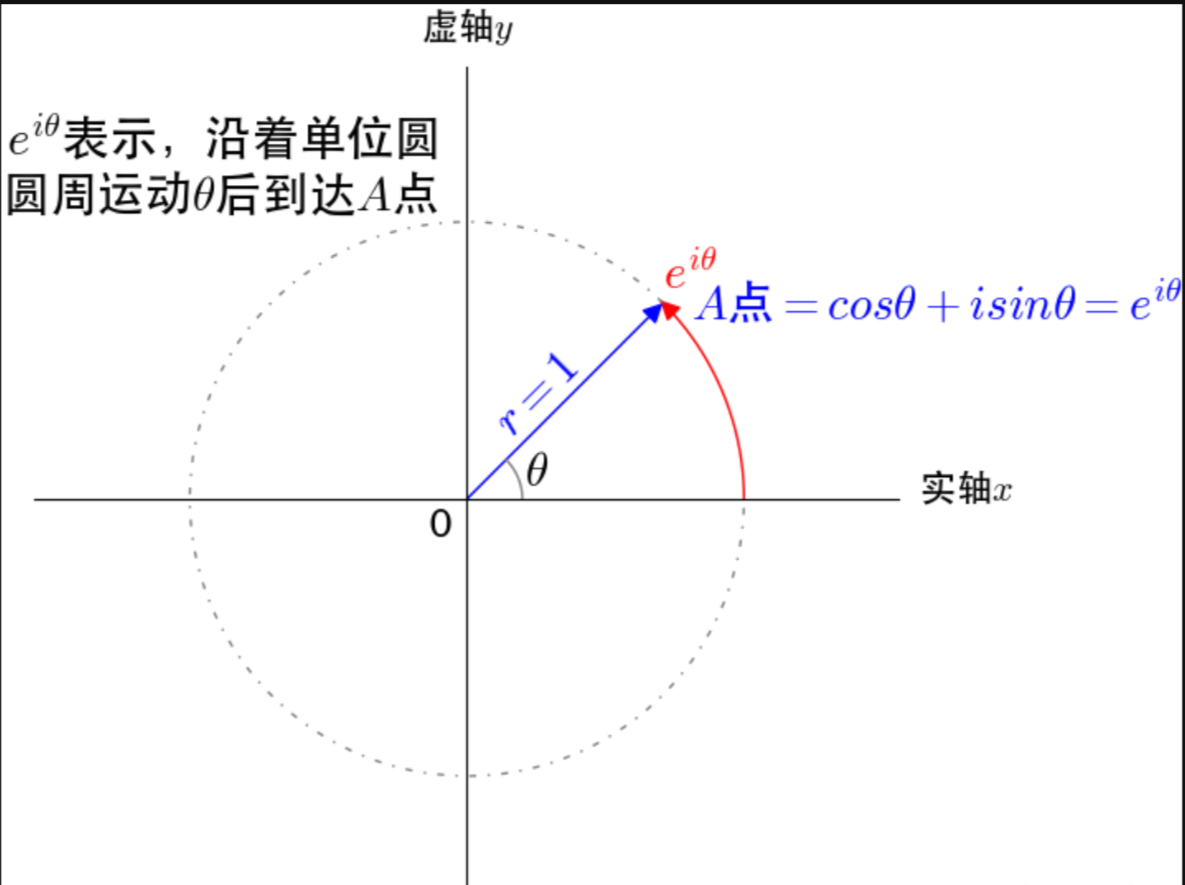
\includegraphics[width=0.45\textwidth]{picture/oula.png} &
    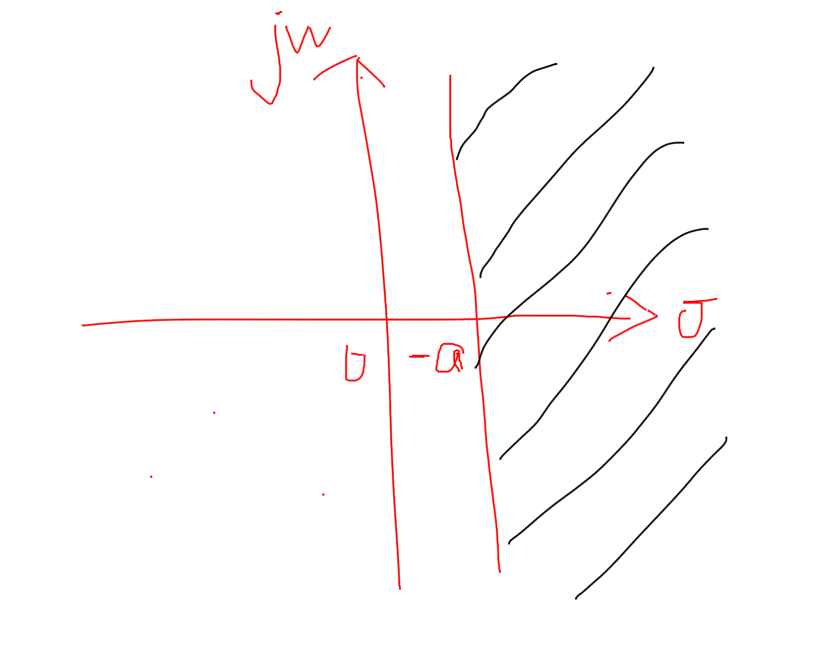
\includegraphics[width=0.45\textwidth]{picture/shoulianyu.png} \\
\end{tabular}
  \end{notitlebox}
  \begin{flushleft}
    虽然拉普拉斯变换拓展了傅里叶变换的适用性,但是也不是所有的函数都可以进行拉普拉斯变换的。拉普拉斯变换要求函数在某个区间内绝对可积。如果函数在$t\rightarrow\infty$ 时振荡剧烈或发散,可能无法满足这一条件,如$f(t)=sin(t^2)$震荡过于剧烈
  \end{flushleft}

  \subsubsection{拉普拉斯性质}
   \begin{titlebox}{线性性质、尺度变换特性}
    1、线性性质
     \\若$\mathcal{L}\left[ f_1\left( t \right) \right] =F_1(s)$ ,$\mathcal{L}\left[ f_2\left( t \right) \right] =F_2(s)$ 
     \\则$\mathcal{L}[a_1 f_1(t) +a_2 f_2(t)] =a_1F_1(s)+a_2F_2(s)$ 
    \\2、尺度变换
    \\若$\mathcal{L}\left[ f\left( t \right) \right] =F(s)$
    \\则$\mathcal{L}[ f( at ) ] =\dfrac{1}{a}F(\dfrac{s}{a})$
   \end{titlebox}

   \begin{titlebox}{时移特性、复频移特性}
    1、时移特性
    \\若$\mathcal{L}\left[ f\left( t \right) \right] =F(s)$
    \\则$\mathcal{L}\left[ f\left( t-t_0 \right) \right] =F(s)e^{-st_0}$
    \\2、复频移特性
    \\若$\mathcal{L}\left[ f\left( t \right) \right] =F(s)$
    \\则$\mathcal{L}\left[ f\left( t \right)e^{s_0t} \right] =F(s-s_0)$
   \end{titlebox}
   \begin{titlebox}{微积分性质}
    1、微积分性质
   \\若$\mathcal{L}\left[ f\left( t \right) \right] =F(s)$
   \\则$\mathcal{L}\left[ f'\left( t \right) \right] =sF(s)-f(0_-)$,$\mathcal{L}\left[ f''\left( t \right) \right] =s^2F(s)-sf(0_-)-f'(0_-)$
   \\若$f(t)$是因果系统:
   \\则\ $\mathcal{L}\left[ f^{(n)}(t) \right] =s^nF(s)$
   \\{\scriptsize 什么是因果系统呢?系统在某时刻t的输出仅取决于时刻t及在t之前的输入,而与 t之后的输入无关,简单来说就是我打你一巴掌让你脸疼,肯定是我现在或者之前打的你,不可能是未来的我打你导致你现在疼。我们生活中的系统都是因果系统所以上面的式子很重要}
   \\2、积分性质
   \\若$\mathcal{L}\left[ f\left( t \right) \right] =F(s)$
   \\则$\mathcal{L}[\int_0^t{f(x)}dx] =\dfrac{1}{s}F(s)$
   ,$\mathcal{L}[(\int_0^t)^n{f(x)}dx] =\dfrac{1}{s^n}F(s)$
   \end{titlebox}
   \begin{titlebox}{终值定理}
    定义:$f(t)$当$t\rightarrow\infty$存在,且$\mathcal{L}\left[ f\left( t \right) \right] =F(s)$,$Re[s]>\sigma_0$,$\sigma_0<0$,则$f(\infty)=\underset{s\rightarrow 0}{\lim}sF\left( s \right) $
    \\{\scriptsize 这个定理很有用,当你将系统进行拉普拉斯变换后,它可以利用终值定理判断该系统是否稳定,并且趋于哪个值。这个后面我在证明的时候会用上,大家可以留意一下。}
   \end{titlebox}
   \begin{flushleft}
    上面的定理都可以代入拉普拉斯的定义进行证明,只是考大家的高数能力而已,在这我就不花过多的篇幅进行证明了。下面讲的卷积定理很重要,所以我会附上证明过程,而上面的性质大家只需背记即可。
   \end{flushleft}
   \begin{titlebox}{卷积定理}
    \begin{center}
      $\mathcal{L}[f(t)*g(t)] =F(s)\cdot G(s)$
    \end{center}
    证:
    \begin{align*}
      \mathcal{L}[f(t)*g(t)] &= \int_0^{\infty} \left( f(t) * g(t) \right) e^{-st} \, dt \\
                              &= \int_0^{\infty} \left( \int_0^t f(\tau) g(t - \tau) \, d\tau \right) e^{-st} \, dt
    \end{align*}
    \begin{flushleft}
      这是一个二重积分,可以用交换积分顺序与上下限的方式来进行化简
      \begin{align*}
         \int_0^{\infty} \left( \int_0^t f(\tau) g(t - \tau) \, d\tau \right) e^{-st} \, dt=\int_0^{\infty}  \int_\tau^{\infty} f(\tau) g(t - \tau) e^{-st}\, dt   \, d\tau  \  \textbf{(a)}
      \end{align*}
      对$  \int_\tau^{\infty} f(\tau) g(t - \tau) e^{-st}\, dt   \, d\tau$进行使用换元法,令$t-\tau=u$,得(使用换元法的原因是我们需要将函数里面的变量分开,进行解耦)
      \begin{align*}
         & t=u+\tau\\      
       \Rightarrow & dt=du+d\tau=du\\
       \Rightarrow  &\int_\tau^{\infty} f(\tau) g(t - \tau) e^{-st}\,   dt   \, d\tau=\int_0^{\infty} f(\tau) g(u) e^{-s(u+\tau)}\,   du   \, d\tau  \ \textbf{(b)}
      \end{align*}
        {\scriptsize这里积分上下限变的原因是原本t的积分范围是$(\tau,\infty)$,而$u=t-\tau$,所以很自然的u的积分范围就是$(0,\infty)$}
        \\将\textbf{(b)}式代入\textbf{(a)}式得
        \begin{align*}
          \int_0^{\infty}  \int_\tau^{\infty} f(\tau) g(t - \tau) e^{-st}\,   dt   \, d\tau&=\int_0^{\infty}\int_0^{\infty} f(\tau) g(u) e^{-s(u+\tau)}\,   du   \, d\tau  \\
          &=\int_0^{\infty} f(\tau) e^{-s\tau}\,   d\tau \cdot \int_0^{\infty} g(u)e^{-su} du  \ \\
          &=F(s)G(s)
       \end{align*}
    上面在学习卷积的时候我们知道了系统的输出等于输入卷积冲激响应,但是如果每次都需要积分的话运算就会十分复杂,这也是我们将时域分析转换为频域分析的一个原因之一。所以,当我们想求一个系统的输出时,我们就会很自然的将它转换成频域,由卷积运算变为乘法运算降低我们的运算难度。
    \end{flushleft}

   \end{titlebox}
   \subsubsection{拉普拉斯逆变换} 
    \begin{flushleft}
      我们现在知道怎么样将时域转换为频域,那怎么将其频域转换回时域呢,毕竟频域只是我们分析的一个方法,我们更加擅长于看时域的东西。所以,当我们利用频域分析完了一个系统之后,得到的结果我们应该学会转换回时域。
      \\将拉普拉斯逆变换主要有四个方法,①定义,②查表,③性质,④分式展开。定义是利用拉普拉斯反变换的定义式进行计算,由于计算复杂我们一般都不会用定义式来算。查表就是那些直接可以在我上面提供的拉普拉斯变换公式表里面可以查到的,所以主要教大家如何利用拉普拉斯的性质和分式展开来进行逆变换。
    \end{flushleft}
    \begin{titlebox}{拉普拉斯逆变换定义式}
      \begin{align*}
        f(t)=\mathcal{L}^{-1}[F(s)]=\dfrac{1}{2\pi j}\int_{\sigma -j\infty}^{\sigma +j\infty}{F\left( s \right)}e^{st}ds
      \end{align*}    
      其中:$\sigma$ 是实常数
       \\这里只是简单提一下,让大家知道有这个东西就行,很少用
    \end{titlebox}
    下面就通过一些例题给大家讲解一下怎么样使用性质和分式展开进行拉普拉斯逆变换。
    \begin{flushleft}
      \begin{notitlebox}
         \ 当我们拿到一个s域的函数$F(s)$时,我们需要确定我们展开的式子是真分式,如果不是的话就化成真分式,这里的真分式是指分母最高幂次大于分子。
    \begin{align*}
      F(s)=P(s)+F_1(s)
    \end{align*}
    其中$P(s)$为整式,$F(s)$为真分式
   \\\textbf{①} 先解$P(s)$,例如当$P(s)=a_2s^2+a_1s+a_0$
    \\查表得,$\mathcal{L}[\delta(t)]=1$,由微分性质得,
    \begin{align*}
      P(s)=a_2 \delta''(t)+a_1\delta'(t)+a_0\delta(t)
    \end{align*}
   \textbf{②} 再求$F_1(s)$,将$F_1(s)$进行分解
      \begin{align*}
        F_1(s)=\dfrac{B(s)}{A(s)}=\dfrac{k_1}{s-p_1}+\dfrac{k_2}{s-p_2}+...+\dfrac{k_i}{s-p_i}
      \end{align*}
      对每个k进行求解,
      \begin{align*}
        k_i=(s-p_i)F(s)\mid_{s=p_i}^{}
      \end{align*}
      再对每个分式用性质和查表进行求逆
      \begin{align*}
        \mathcal{L}^{-1}[\dfrac{k_i}{s-p_i}]=k_ie^{p_it}\varepsilon (t)
      \end{align*}

     
      \begin{flushleft}
        $A(s)$称为$F_1(s)$的特征多项式,$A(s)=0$为特征方程,它的根为特征根,\textbf{特征根$p_i$也称为$F(s)$的极点}。可能有些迷,下面直接解一道题给大家看一看。
        \vspace{1cm}
        \\例:$F(s)=\dfrac{s^2+5}{s^2
        +5s+4}$,求逆变换
        \\由式子我们得出F(s)为假分式,用长除法将式子化为真分式得
        \begin{align*}
          F(s)&=P(s)+F_1(s)\\
              &=1+\dfrac{-5s+1}{s^2+5s+4}
        \end{align*}
        $P(s)$由查表得,
        \begin{align*}
          p(t)=\mathcal{L}^{-1}[P(s)]= \mathcal{L}^{-1}[1]=\delta(t)
        \end{align*}
        对$F_1(s)$进行分解:
        \begin{align*}
          F_1(s)&=\dfrac{-5s+1}{s^2+5s+4}\\
              &=\dfrac{-5s+1}{(s+1)(s+4)}=\dfrac{k_1}{(s+1)}+\dfrac{k_2}{(s+4)}\\
            k_1&=(s+1)F(s)\mid_{s=-1}^{}\\
              &=\dfrac{-5s+1}{(s+4)}\mid_{s=-1}^{}\\  
              &=2
        \end{align*}
        同理可得,$k_2=-7$
        \\所以,$F_1(s)=\dfrac{2}{(s+1)}+\dfrac{-7}{(s+4)}$
        \begin{align*}
          f_1(t)&=\mathcal{L}^{-1}[F(s)]=(2e^{-t}-7e^{-4t})\varepsilon (t)
        \end{align*}
        所以,最后将两个式子加在一起就是我们所求的了
        \begin{align*}
          f(t)&=p(t)+f_1(t)\\
               &=\delta(t)+(2e^{-t}-7e^{-4t})\varepsilon (t)
        \end{align*}
      \end{flushleft}
    \end{notitlebox}
    上面的是单根的情况,如果出现了重根我们又应该怎么去算呢?
    
    \begin{notitlebox}
      \ 重根的解法:
      \begin{align*}
        F(s)=\dfrac{A(s)}{B(s)}=\dfrac{K_{11}}{\left( s-p_1 \right) ^r}+\dfrac{K_{12}}{\left( s-p_1 \right) ^{r-1}}+...+\dfrac{K_{1r}}{\left( s-p_1 \right) }
      \end{align*}
      \\利用下面公式可以直接得到每个系数
      \\$K_{11}=[\left( s-p_1 \right) ^r F(s)]\mid_{s=p_1}^{}$
      \vspace{0.5cm}
      \\$K_{12}=\dfrac{d[\left( s-p_1 \right) ^r F(s)]\mid_{s=p_1}^{}}{ds}$
      \vspace{0.5cm}
      \\$K_{1r}=\dfrac{1}{(r-1)!}\dfrac{d^{r-1}}{ds^{r-1}}[\left( s-p_1 \right) ^r F(s)]\mid_{s=p_1}^{}$
      \\给大家一个具体的例题来看看是怎么用的:
      \begin{center}
        $F(s)=\dfrac{s-2}{s(s+1)^3}$,求逆变换  
      \end{center}
      解:
      \begin{align*}
        &\text{设}F(s)=\dfrac{k_{11}}{(s+1)^3}+\dfrac{k_{11}}{(s+1)^2}+\dfrac{k_{11}}{(s+1)}+\dfrac{k_2}{s}\\
        &\text{令}F_1(s)=(s+1)^3F(s)=\dfrac{s-2}{s}\\
        &k_{11}=F_1(s)\mid_{s=-1}{}=\dfrac{s-2}{s}\mid_{s=-1}=3\\
        &k_{12}=\dfrac{dF_1(s)}{ds}\mid_{s=-1}{}=\dfrac{s-(s-2)}{s^2}\mid_{s=-1}=2\\
        &k_{13}=\dfrac{1}{2}\dfrac{d^2F_1(s)}{ds^2}\mid_{s=-1}{}=\dfrac{1}{2}\cdot\dfrac{-4s}{s^4}\mid_{s=-1}=2\\
        &k_{2}=sF(s)\mid_{s=0}{}=\dfrac{s-2}{(s+1)^3}\mid_{s=0}=-2\\
        &\therefore F(s)=\dfrac{3}{(s+1)^3}+\dfrac{2}{(s+1)^2}+\dfrac{2}{s+1}-\dfrac{2}{s}\\
         &f(t)=\mathcal{L}^{-1}[F(s)]=(\dfrac{3}{2}t^2e^{-t}+2te^{-t}+2e^{-t}-2)\varepsilon(t) 
      \end{align*}
      
    \end{notitlebox}
    
  \end{flushleft}

    \subsection{传递函数和系统的设计}
    当我们知道了什么是频域、什么是拉普拉斯变换之后,我们就可以开始学什么是传递函数了,它是我们经典控制理论的基础,可以理解为它是由我们时域上的系统通过拉普拉斯变换转换成频域之后的一种表达式。
    \subsubsection{传递函数}
    \begin{titlebox}{什么是传递函数}
      传递函数是描述线性系统动态特性的数学工具,主要用途是描述系统特性,分析系统响应,设计控制系统,判断系统稳定性
      \\定义:在零初始条件下,\textbf{系统输出的拉普拉斯变换与系统输入的拉普拉斯变换之间的比值},即
      \begin{align*}
        G(s)=\dfrac{X(s)}{U(s)}
      \end{align*}
        上式的系统可以用如下框图表示\\
        \begin{center}
            \begin{tikzpicture}[node distance=4cm]
          \node (start) [startstop] {$U(s)$};
          \node(input)[sys,right of=start]{$G(s)$};
          \node (output) [process, right of=input, xshift=0cm] {$X(s)$};
          \draw [arrow] (start) -- (input);
          \draw [arrow] (input) -- (output);
        \end{tikzpicture}
        \end{center}
        \begin{align*}
          X(s)=\mathcal{L}[u(t)*g(t)]=U(s)G(s)
        \end{align*}
     显而易见,我们将系统和输入之间的关系从卷积转换成了乘法
     {\scriptsize\\上面我说过一句话:冲激响应可以完全定义系统。在这里我们可以从频域的角度来看,
     \\令输入$u(t)=\delta (t)$
     \begin{align*}
      X(s)=U(s)\cdot G(s)&=\mathcal{L}[\delta (t)]\cdot G(s)\\
                         &=G(s)
     \end{align*}
     这里可以更清楚的看到系统的冲激响应等于传递函数(系统本身)}
              
    \end{titlebox}
    现在我可以用频域分析给大家分析一下上面的弹簧质量阻尼系统了
    \begin{notitlebox}
          \par 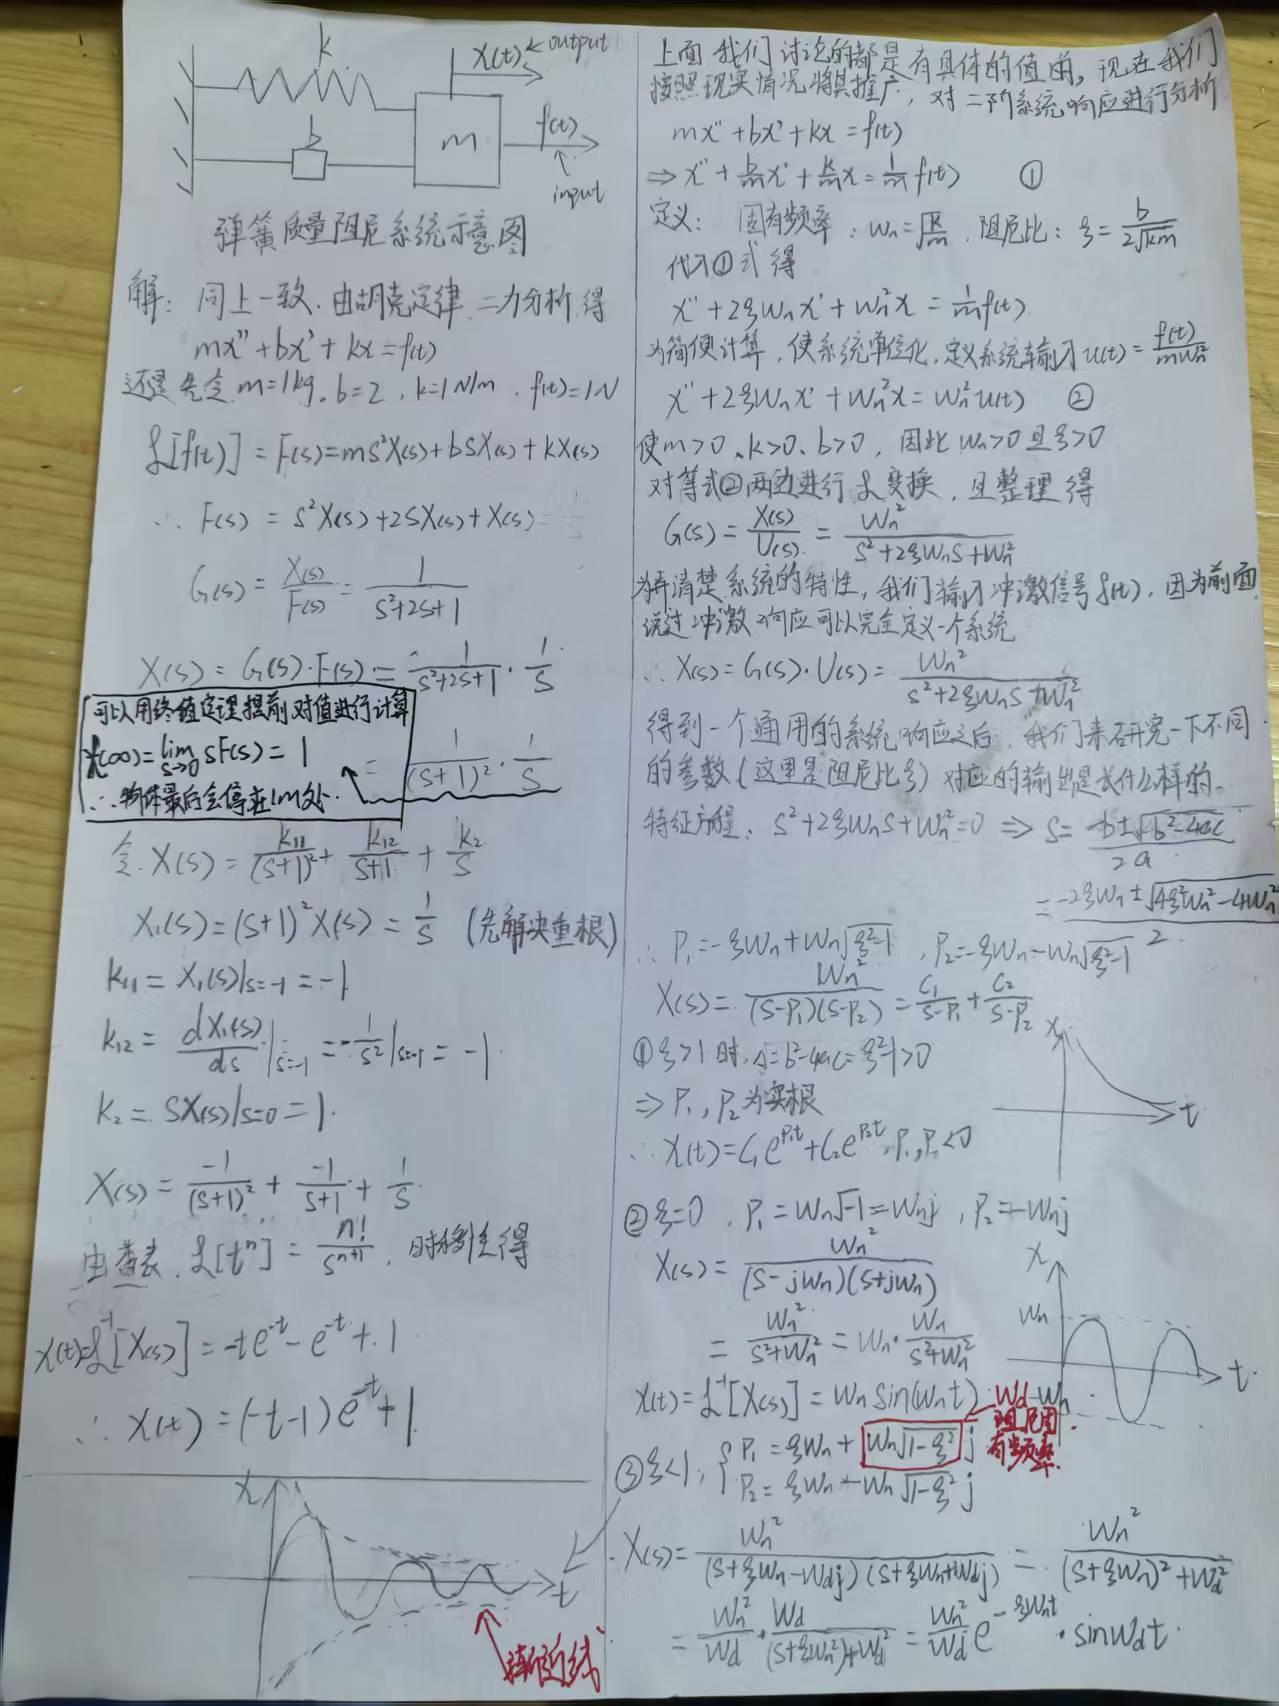
\includegraphics[width=10cm]{picture/transform formula.png}
   \\ 对于不同的阻尼比,我们得到不同的系统冲激响应。
   \\{\scriptsize 下面说的系统是对所有二阶系统都适用}
    \\①当$\xi>1$时,系统称为过阻尼系统,其响应不会出现震荡,且快速收敛
    \\②当$\xi=1$时,系统称为界阻尼系统,处于震荡的临界。
    \\②当$0<\xi<1$时,系统称为欠阻尼系统,其响应会不断地振动且幅度逐渐减少并最终停下来。
    \\③当$\xi=0$时,系统称为无阻尼系统,他会一直振动下去,且不会消耗能量。
    \\我们很容易看出对于系统的最终响应,表面上改变的是$\xi=0$,但究其原因是极点的改变,导致系统的响应变化。
    \\我们看到的系统基本是分式的形式,当$\dfrac{k}{s-p}$进行拉式反变换的时候,得到的一定是$ke^{pt}$的形式,从这里我们可以看出系统是否震荡、是否收敛、收敛快慢、都会取决于极点(系统的整式部分不影响我上面说的)。这里我只是简单的铺垫一下,后面会有更详细的解释。
    \end{notitlebox}
    

    \subsubsection{系统设计}
    大家上面看到的都是一个单纯的系统,是不包含控制器的,接下来我就给大家开始讲关于控制系统传递函数。
    \begin{titlebox}{开环控制系统}
      \begin{flushleft}
        下图就是开环控制系统:其中R(s)是\textbf{参考值}或目标值,C(s)是控制器,原动态系统的传递函数G(s)被称为控制系统的\textbf{开环传递函数}。控制量是U(s),也就是原动态系统的输入。控制系统的输出等于原动态系统的输出X(s)。
      \end{flushleft}
       \par 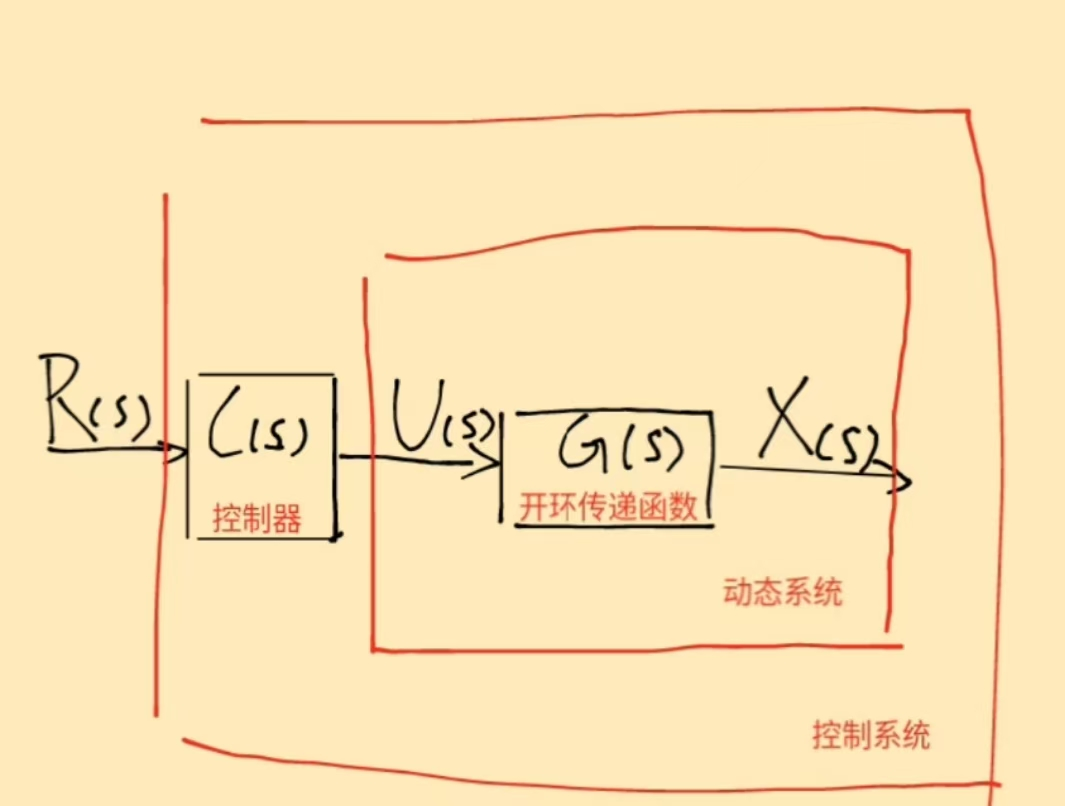
\includegraphics[width=10cm]{picture/control system.png}
      \begin{flushleft}
        开环控制系统就是我们只管输入值,对输入值进行控制,达到我们的预设值。即使有误差我们也不管,也管不了,因为系统里面不存在反馈,控制器是不知道最后输入的结果的。
      \end{flushleft}


    \end{titlebox}
    若将X(s)反馈到输入端,则可以形成一个闭环控制系统
  \begin{titlebox}{闭环传递函数}
    \par 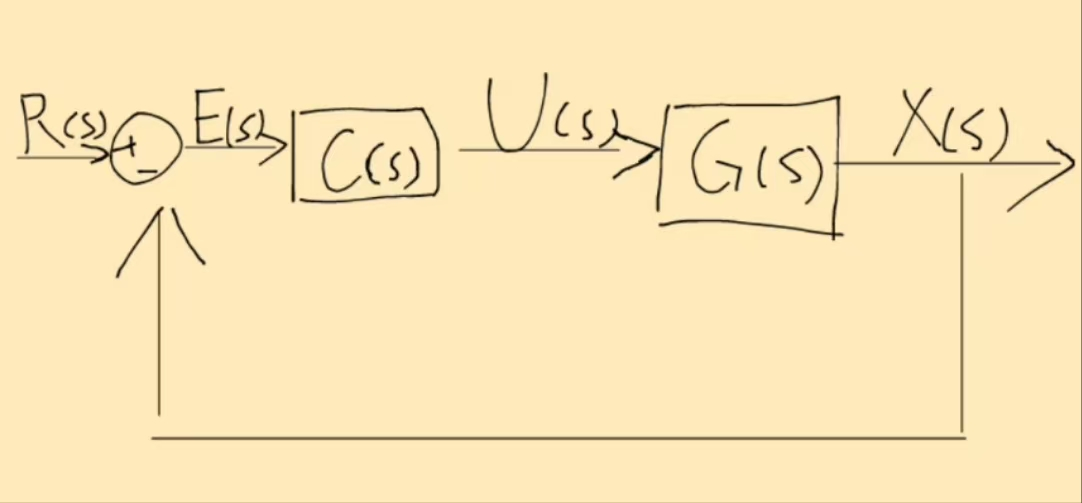
\includegraphics[width=12cm]{picture/feedback control.png}
    \\其中,参考值与输入之间的差称为误差,$E(s)=R(s)-X(s)$,其对应的时间函数是$e(t)=r(t)-x(t)$,控制器C(s)根据误差决定控制量U(s)。
    \\根据传递函数的代数性质,可得
    \begin{align*}
      X(s)=U(s)G(s)=E(s)C(s)G(s)
    \end{align*}
    将$E(s)=R(s)-X(s)$带入上式得,
    \begin{align*}
      &X(s)=(R(s)-X(s))C(s)G(s)\\
      \Rightarrow&(1+C(s)G(s))X(s)=R(s)C(s)G(s)\\
      \Rightarrow&X(s)=\dfrac{C(s)G(s)}{1+C(s)G(s)}
    \end{align*}
    定义控制系统的闭环传递函数为
    \begin{align*}
      G_{cl}(s)=\dfrac{X(s)}{R(s)}=\dfrac{C(s)G(s)}{1+C(s)G(s)}
    \end{align*}
    所以我们可以得到一个简化后的闭环控制系统框图\\
    \begin{center}
      \begin{tikzpicture}[node distance=5cm]
      \node (start) [startstop] {$R(s)$};
      \node(input)[sys,right of=start]{$ G_{cl}(s)==\dfrac{C(s)G(s)}{1+C(s)G(s)}$};
      \node (output) [process, right of=input, xshift=0cm] {$X(s)$};
      \draw [arrow] (start) -- (input);
      \draw [arrow] (input) -- (output);
    \end{tikzpicture}
    \end{center}
    从这里我们也可以看到,我们设计和调整控制器根本上就是改变传递函数的极点和零点\\
    注意:此处的开环传递函数是针对闭环系统来说的,不是开环系统的传递函数。\\
    由上面分析可知开环传递函数和闭环传递函数关系紧密,因此系统的开环频率特性很大程度上决定了系统的闭环性能。由于闭环系统包含反馈,校准过程较为复杂,而开环传递函数容易分析和设计,因此工程上常用开环传递函数来分析和设计控制器。\label{sec:part1}
  \end{titlebox}
    
  \section{实践知识}
    有了上面的基础知识之后,这一部分我会在实际的运用中,边教大家设计控制器边补全大家所需要的知识。接下来我们就是围绕着如何对我们的云台系统进行仿真和制作控制器。
  \\对解决动态系统的控制问题我们可以从如下三个部分入手
  \begin{notitlebox}
    \par 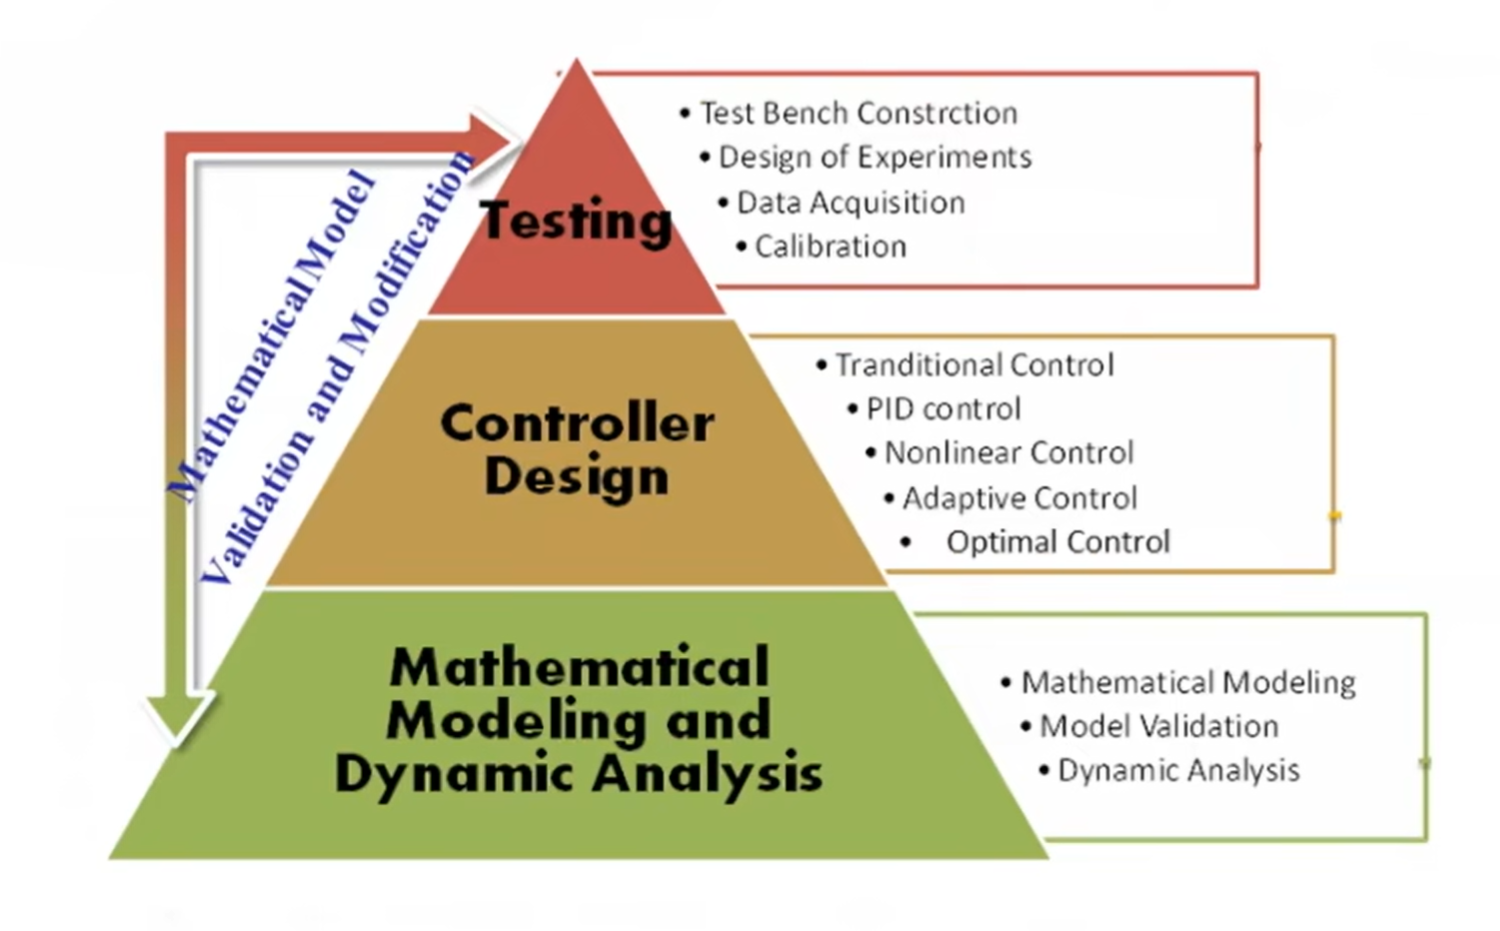
\includegraphics[width=12cm]{picture/controller_pyramid.png}
    \textbf{Mathematical Modeling and Dynamic Analysis:}对研究的对象进行分析,研究其物理特性,然后进行数学建模,得出系统的传递函数。\\
    \textbf{Contronller Design:}为满足不同的要求(如响应快,震荡小等),我们要用多种控制原理的工具,在数学建模的基础上进行控制器的设计\\
    \textbf{Testing:}最后便是在仿真平台或者实物上进行测试
  \end{notitlebox}
  \subsection{系统传递函数}
    要对我们的云台进行控制器的设计首先我们需要先建模出一个系统
    Yaw轴云台的转角关于输入力矩是一个二阶的模型
    \begin{align*}
       J\overset{..}{\theta}+b\overset{.}{\theta}=T
    \end{align*}
    而Yaw轴云台的角速度关于输入力矩就是一个一阶的模型
    \begin{align*}
      J\overset{.}{\omega}+b\omega =T
    \end{align*}
    \begin{flushleft}
      (其中J是云台转动惯量,b是阻尼系数,这二者可认为是常数,而T是我们控制输入的力矩,具体的推导过程就留给大家尝试,需要一定的大物知识)
    但是由于我们云台电机磨损情况不知、难以准确的得到转动惯量和阻尼系数,所以我们要借助Matlab的system identification工具进行系统识别。\\
   \subsubsection{实现步骤}
      \begin{flushleft}
        \textbf{第①步:扫频}\\
        \ 首先我们需要扫频,扫频就是说我们系统输入的信号需要从1-40Hz增加,从而得到每个频率对应的响应。
      \end{flushleft}

       \begin{flushleft}
        我们需要在云台代码中加入以下的代码
       \end{flushleft}
      %  \begin{lstlisting}
      %   float Sweep(debug_wave_t *Debug_wave)
      %   {
      %     static u32 i_fre = 0;
      %     float w,speed_ref,omg;
      %     uint32_t N;
      %       if(Sweep_type == Sine)
      %       {
      %         \\ TIM_FRE 为函数执行频率,等效于采样频率 
      %          omg tbackslash 数字角频率 
      %   }= sweep_fre_sine[i_fre]*_2pi;\tex
      % \end{lstlisting}
      \par 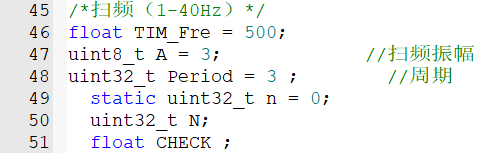
\includegraphics[width=12cm]{picture/sweep_1.png}
      \par 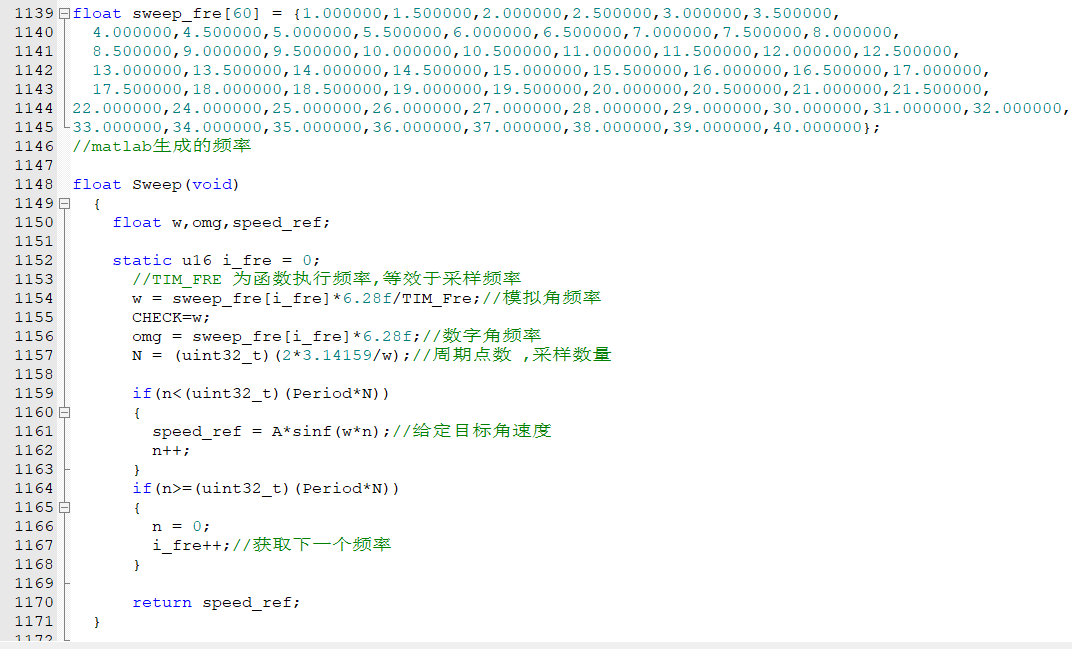
\includegraphics[width=12cm]{picture/sweep_2.png}
      \begin{flushleft}
        上面的数组不用自己一个一个的敲,可以用matlab生成。\\
        \textbf{根据经验和时域的响应情况,调节PID参数使得云台可以较为稳定的跟随目标角速度。}然后记住将速度环的输入改为我们的扫频信号
      \end{flushleft}
      \par 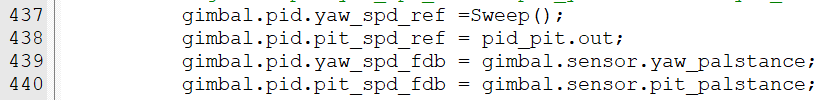
\includegraphics[width=12cm]{picture/sweep_3.png}
      \begin{flushleft}
        \textbf{第②步:采集数据、导入数据}\\
        我们只需要用vofa+来采集数据就好了
        \par 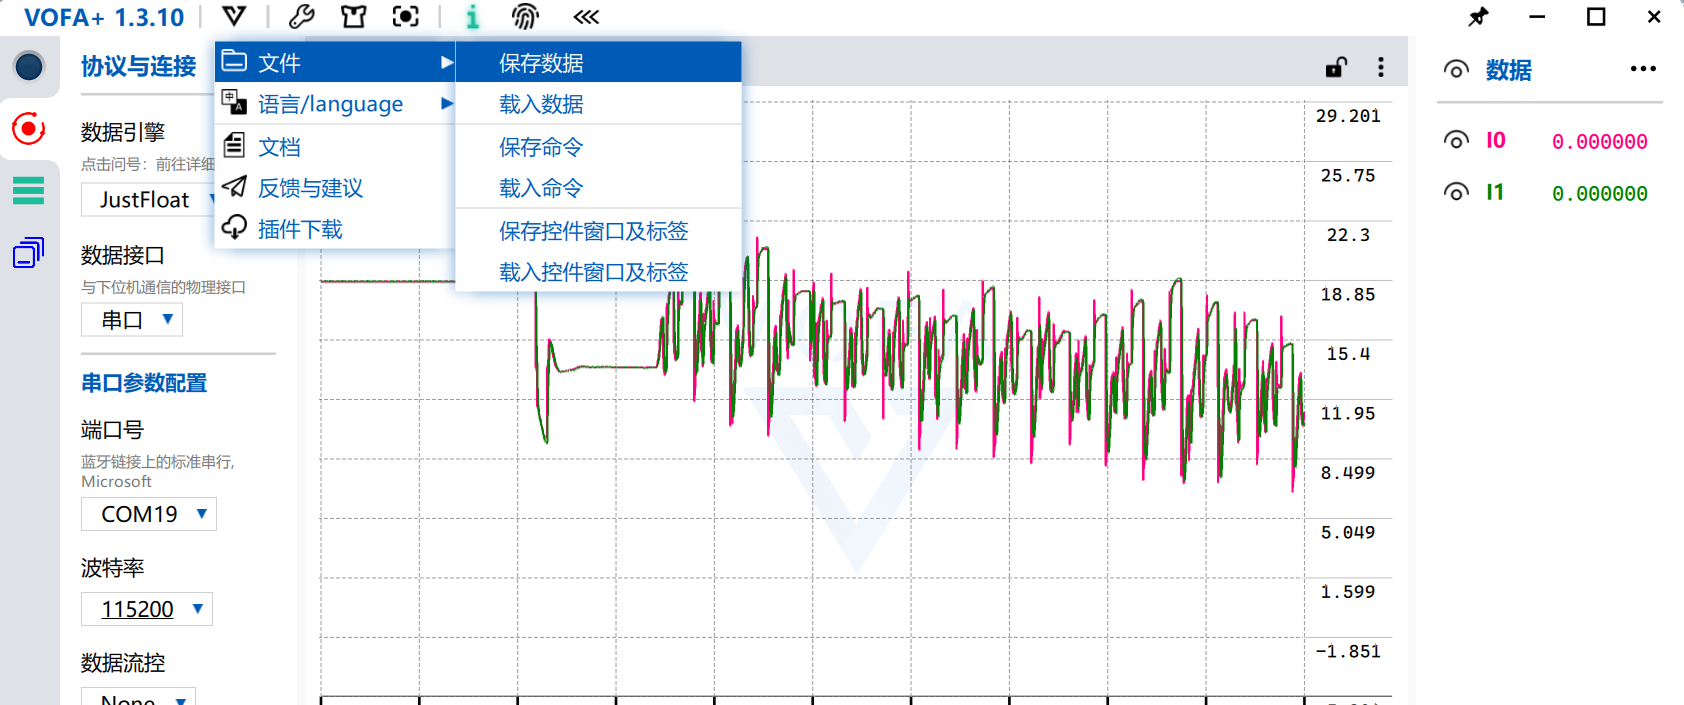
\includegraphics[width=12cm]{picture/collection.png}
      \end{flushleft}
      \begin{flushleft}
        在matlab上方的菜单中选择导入数据选项
        \par 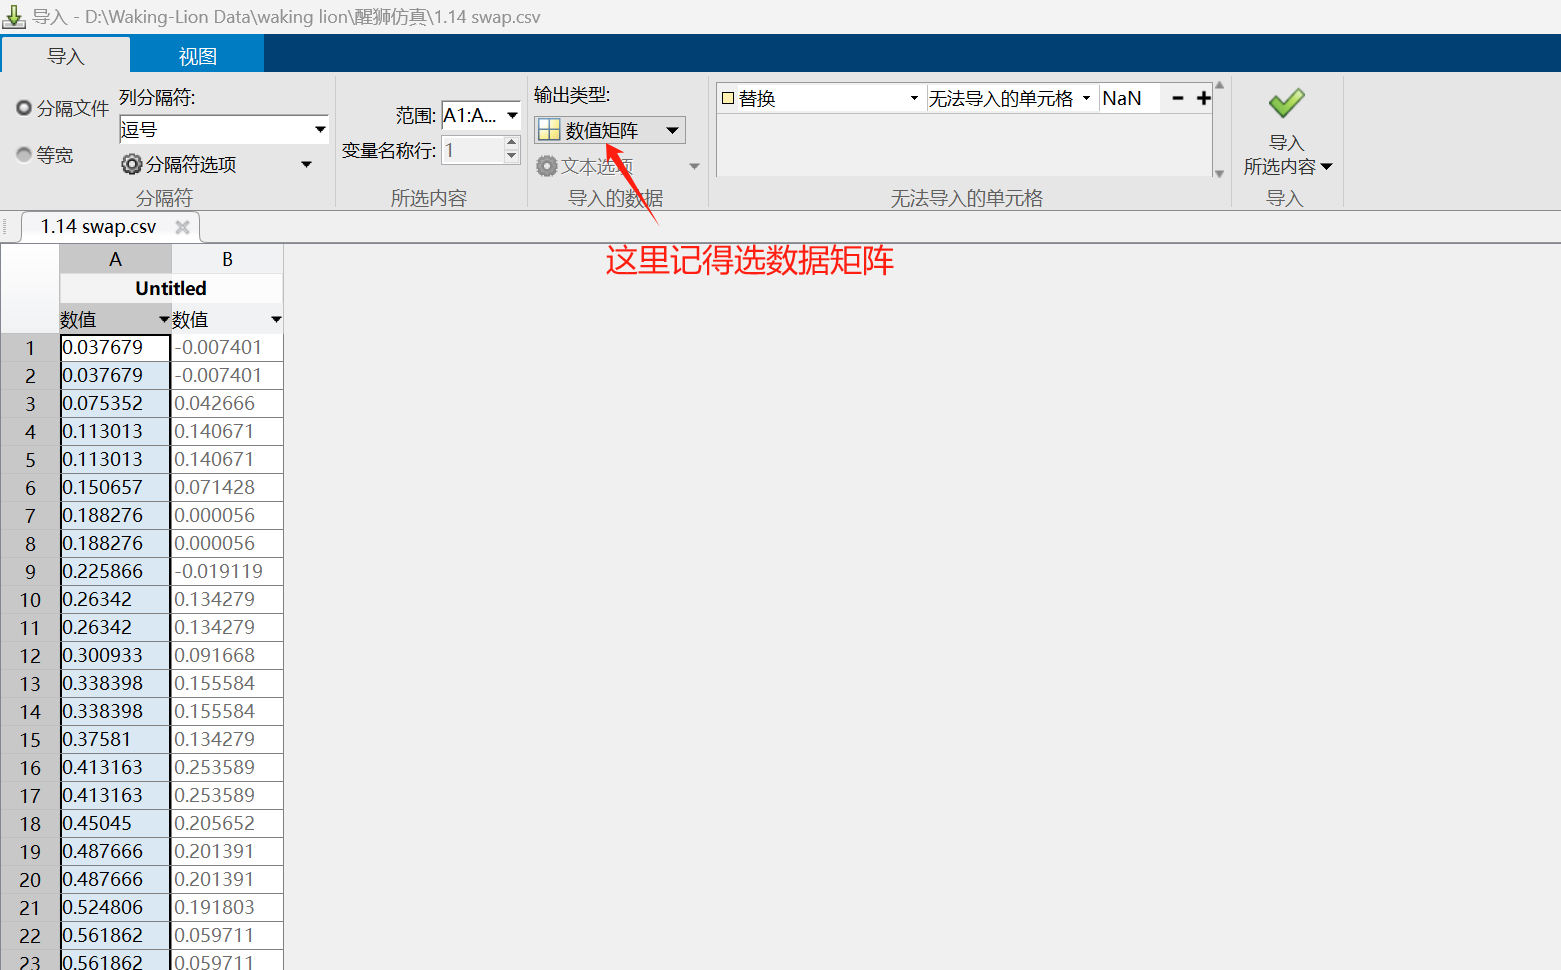
\includegraphics[width=12cm]{picture/data_impot.png}
        \par 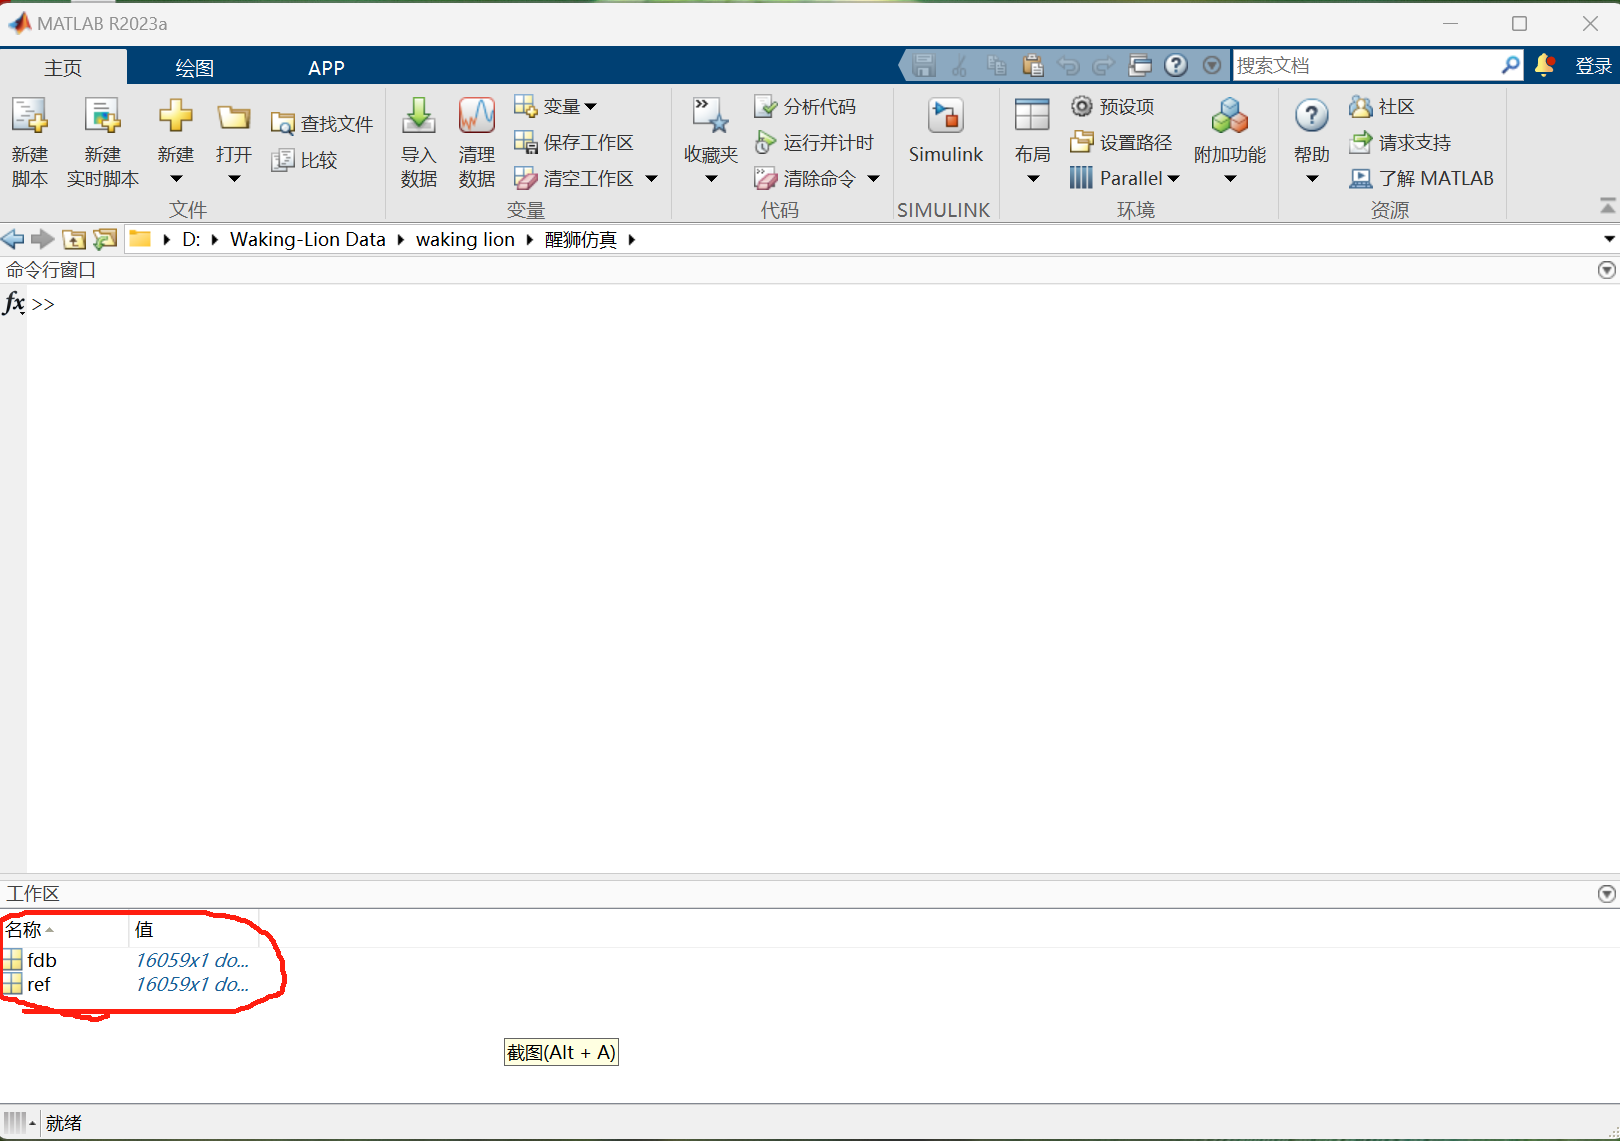
\includegraphics[width=12cm]{picture/data_impot1.png}
        \\留意工作区的变量,记得自己修改名字。
        \\将两组数据导入后我们就可以进行下一步了
      \end{flushleft}
      \begin{flushleft}
        \textbf{第③步:系统识别}\\
        找到并打开system Identification工具箱,选择 Import data > Time domain data ,打开导入数据对话框,在 input 和 output 选项中键入工作区的输入输出变量名,Starting time 和 Sample time 分别输入 0 和 0.003(这个采样时间需要自己确定,往下看)。其他部分选填。点击 Import 将数据加入System Identification工具,然后关闭对话框。
      \end{flushleft}
      \begin{flushleft}
        
        \par 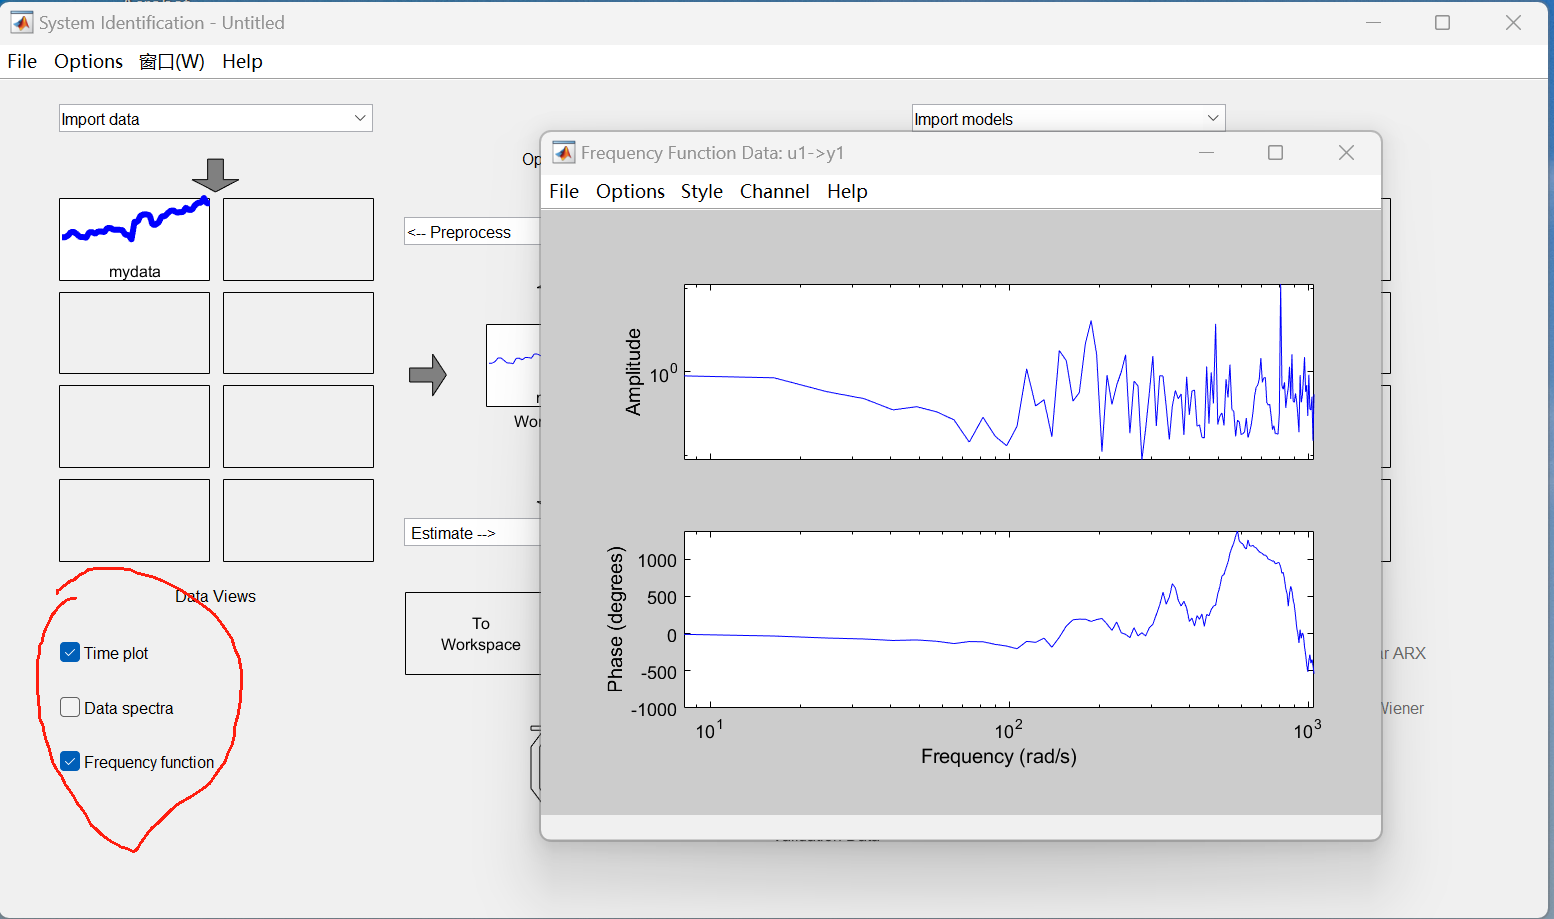
\includegraphics[width=12cm]{picture/bode.png}
        注意勾选上面的选项,来查看输入数据对应的bode图,假若图像如图属于正常状态(虽然很丑),因为对于我们的云台系统而言,前面的低频时是基本符合规律的,而后面频率过高云台响应跟不上输入的信号,就可能会出现这种奇怪的图像。
      \end{flushleft}
      \begin{flushleft}
        直接选择 Estimate > Transfer Function Models 打开传递函数对话框,设置零极点个数分别0和1,点击 Estimate ,得到系统传递函数。
        \par 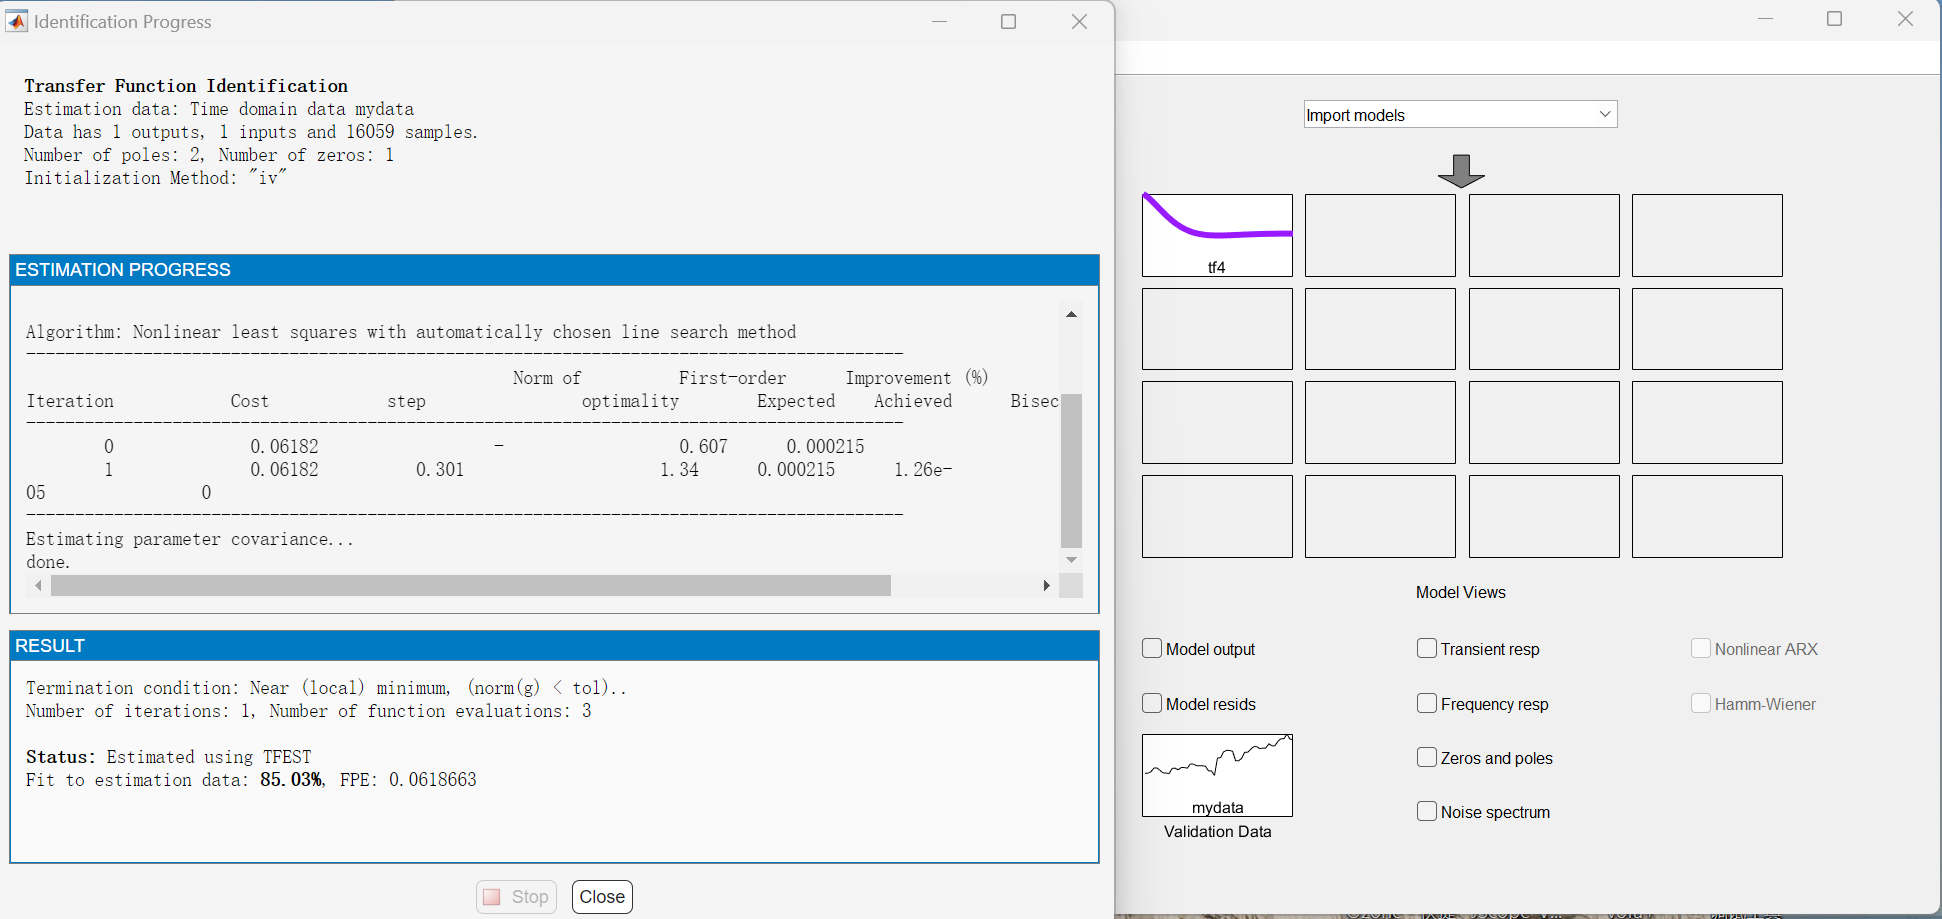
\includegraphics[width=12cm]{picture/identify_result.png}
      \end{flushleft}
      至此,我们的系统就识别出来了
    \end{flushleft}
    

    \href{https://bbs.robomaster.com/wiki/4574/3559}{RM官方开源教程-系统辨识基础教程}
    \\\href{ https://blog.csdn.net/xiaohejiaoyiya/article/details/105958551?ops_request_misc=%257B%2522request%255Fid%2522%253A%2522d515a96088d8f99093ec8d0b4cb80d62%2522%252C%2522scm%2522%253A%252220140713.130102334.pc%255Fall.%2522%257D&request_id=d515a96088d8f99093ec8d0b4cb80d62&biz_id=0&utm_medium=distribute.pc_search_result.none-task-blog-2~all~first_rank_ecpm_v1~rank_v31_ecpm-1-105958551-null-null.142^v100^pc_search_result_base1&utm_term=%E5%88%A9%E7%94%A8system%20identification%E7%A1%AE%E8%AE%A4%E6%A8%A1%E5%9E%8B&spm=1018.2226.3001.4187}{【Matlab】利用System identification App辨识对象模型}。\\
     \href{https://www.bilibili.com/video/BV1wX7BzVEf6/?spm_id_from=333.1391.0.0&vd_source=b02f21f21dd17ebeef8dac9338c9d06c}{云台参数识别与调试}    
    \subsubsection{知识补充}
    \begin{flushleft}
      大家按照我的步骤做完之后肯定会有很多疑惑,首先为什么用一阶系统,为什么我们仿真要用速度环,而不直接仿真系统的传递函数呢。
      \\先记住我们的6020电机用的是电压控制,然后出门左转看\textbf{云台控制 -- Yaw轴系统辨识与控制器设计},然后再看\textbf{6020电压控制与电流控制的特别说明}
    \end{flushleft}
    \begin{titlebox}{采样时间的确定}
      \begin{flushleft}
         打开bsp\_dwt.c文件,在里面加下面的全局变量,并且在其头文件进行外部声明
      \end{flushleft}
      \par 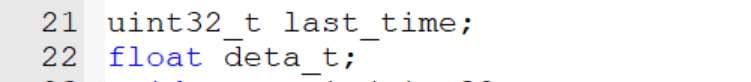
\includegraphics[width=12cm]{picture/variable.png}
      \\
      \begin{flushleft}
        将下面的函数放到vofa+的函数发送上,然后debug看deta\_t这个变量,正常来说是一个定值0.002或0.003
        \par 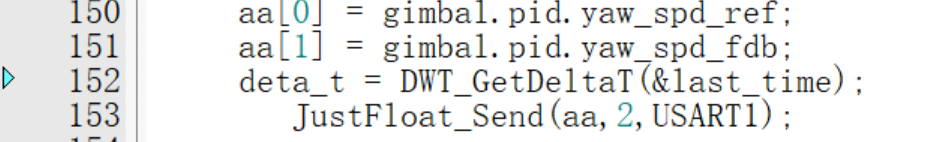
\includegraphics[width=12cm]{picture/variable_1.png}
      \end{flushleft}
    \end{titlebox}
    
    \begin{titlebox}{伯德图的作用}
      伯德图是我们分析系统频率响应的工具,对于一个系统来说输入不同频率的信号其对应输出信号的频率不会变化,但是幅度和相位的大小会发生改变,其改变就是通过伯德图反映出来的。
      
      具体的推导请参考下面的链接:\\
      \href{ https://www.bilibili.com/video/BV1Qb411W7i2?spm_id_from=333.788.videopod.sections&vd_source=b02f21f21dd17ebeef8dac9338c9d06c}{频率响应的推导}\\
      \href{https://www.bilibili.com/video/BV1gx411X7k6?spm_id_from=333.788.videopod.sections&vd_source=b02f21f21dd17ebeef8dac9338c9d06c}{Dr.Can——伯德图}\\
      看完推导后大家一定要记住结论:\\
      \textbf{当正弦输入$u(t)=M_i\cdot sin(\omega_it+\phi)$通过线性时不变系统G(s)后,$\omega_i$不变;振幅变化$|G(j\omega)|$倍,相位移动$\angle G(j\omega)$}\vspace{1cm}
      \label{sec:part2}
     
      在伯德图中我们能看到的东西:
     \begin{flushleft}
       (1) 系统增益\\
     低频增益:反映了系统对直流信号或低频信号的放大能力。
     例如:积分器在低频段增益趋向于无穷大(-20dB/decade)。\\
     高频增益:反映了系统对高频噪声的衰减能力。
     例如:低通滤波器在高频段增益趋向于0。
     \end{flushleft}
     \begin{flushleft}
      (2) 系统的转折频率\\
     幅频特性曲线中,斜率发生变化的位置称为转折频率,通常对应系统中极点或零点的位置。通过转折频率可以辨识系统的动态特性。
     \end{flushleft}
     \begin{flushleft}
       (3) 系统的带宽\\
     带宽是系统能够有效响应信号的频率范围(通常以幅值下降至-3dB处的频率为准)。带宽越大,系统响应速度越快。
     \end{flushleft}
     
    \begin{flushleft}
      (4) 系统的相位滞后\\
     相频特性曲线显示了系统在不同频率下的相位滞后特性:
     \\相位滞后越小,系统响应越快。
     \\相位滞后过大可能导致系统稳定性变差。
    \end{flushleft}
    \vspace{1cm}

     想要深究的同学可以看下面的链接:
     
     \href{https://www.bilibili.com/video/BV1C8UpYaEYN?spm_id_from=333.788.videopod.episodes&vd_source=b02f21f21dd17ebeef8dac9338c9d06c}{伯德图的深入理解}
     
    \end{titlebox}
    \subsection{PID控制器的设计与调参}
    \subsubsection{理论分析}
    \begin{flushleft}
      当我们得到了一个系统之后我们就可以设计控制器进行调参了,PID控制器在理论和实践中都有丰富的经验积累,许多工程问题和解决方案已经得到了深入研究,让我们不需要对大量的控制器进行尝试和筛选,仅需要调参即可。
    \end{flushleft}
    \begin{flushleft}
      但是我们往年来都是进行的经验调参,对PID没有具体的概念和知识,这样会使我们的调参很漫长和痛苦,所以我们需要一些理论的知识来指导我们的实践,从而减少我们调参所需要的时间。
    \end{flushleft}
    \begin{flushleft}
      在经典控制理论中,对于控制器系统的分析我们会有多种的工具,如根轨迹、伯德图、奈奎斯特图等,因为伯德图更加直观和容易理解,所以这里从伯德图的角度,给大家来分析PID控制的本质及其原理。
      
    \end{flushleft}
    \begin{notitlebox}
      \ 首先我们需要有一个概念就是控制器实际上就是改变系统的零点和极点,从而修改系统的频率响应的幅值和相位(\hyperref[sec:part2]{参考上面的频率响应推导结论}),而伯德图正是用来观察系统的频率和相位特性,所以我们会利用伯德图来帮助我们理解PID的控制器。
      \begin{flushleft}
        现在我们有一个一阶系统:
        \begin{align*}
          G(s)=\dfrac{5}{s+5}
        \end{align*}
        我们将要对他进行控制器的设计:
        \par 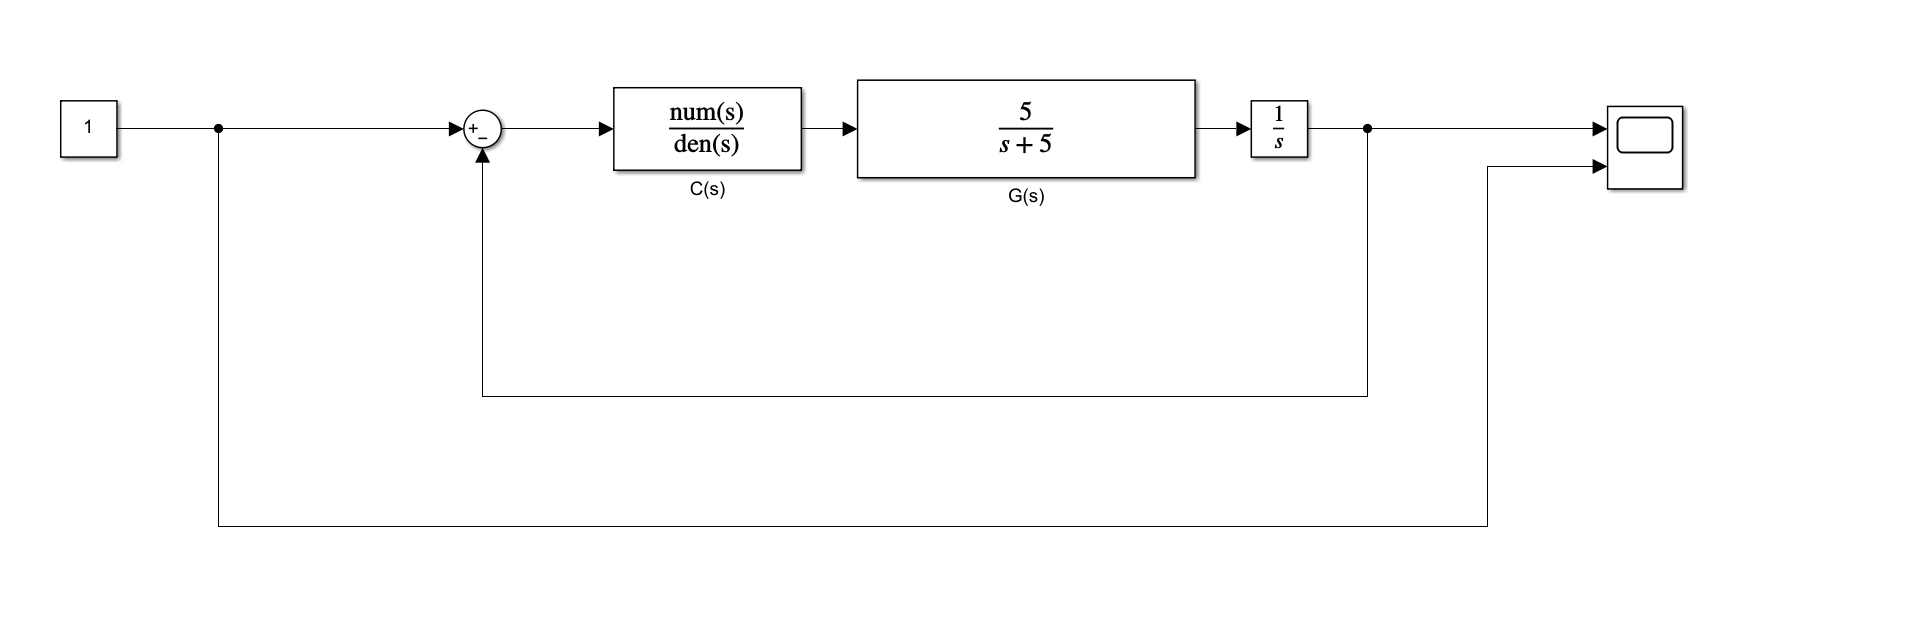
\includegraphics[width=12cm]{picture/matlab.png}
        \\其闭环传递函数为:
      \end{flushleft}
        \begin{align*}
          G_{cl}(s)=\dfrac{C(s)\cdot G(s)}{1+C(s)G(s)}
        \end{align*}
        \begin{center}
          \begin{tikzpicture}[node distance=5cm]
          \node (start) [startstop] {$R(s)$};
          \node(input)[sys,right of=start]{$ G_{cl}(s)==\dfrac{C(s)G(s)}{1+C(s)G(s)}$};
          \node (output) [process, right of=input, xshift=0cm] {$X(s)$};
          \draw [arrow] (start) -- (input);
          \draw [arrow] (input) -- (output);
        \end{tikzpicture}
        \end{center}
      \begin{flushleft}
        当$C(s)=1$时,即没有控制器的情况下,其闭环函数的伯德图如下
        \par 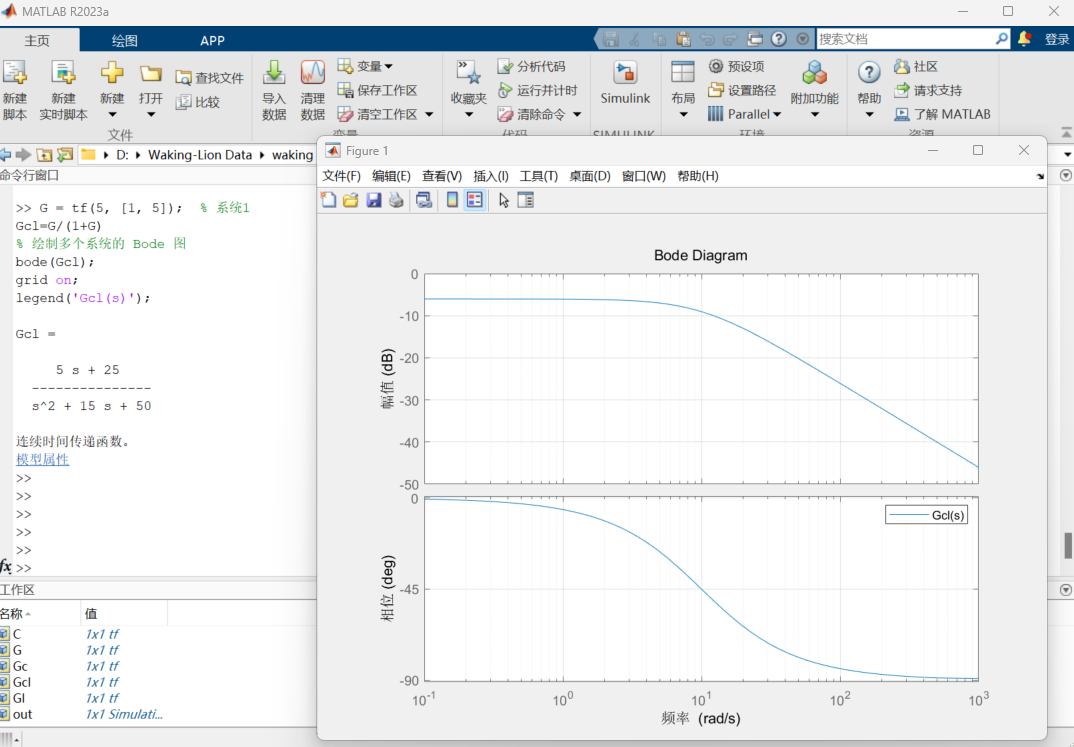
\includegraphics[width=12cm]{picture/close_function.png}
      \end{flushleft}
      \begin{flushleft}
        从伯德图可以看出,系统闭环函数存在一个稳态误差使得$|G_{cl}(j\omega)|<1$具体差多少可以将$j\omega$代入$G_{cl}$中并且取$\omega=0$,得出与参考值相差的倍数。\\
        而且我们还能看出这个系统是一个对高频噪声有良好的抑制效果的系统
        
      \end{flushleft}
      \begin{flushleft}
        我们PID的在s域的表达式为:
        \begin{align*}
          C(s)=K_p+\dfrac{K_i}{s}+K_ds=\dfrac{K_ds^2+K_ps+K_i}{s}
        \end{align*}
      \end{flushleft}
      \begin{flushleft}
        我们先只让$K_p=5$,$K_i=0$、$K_d=0$,可得到伯德图如下:
        \par 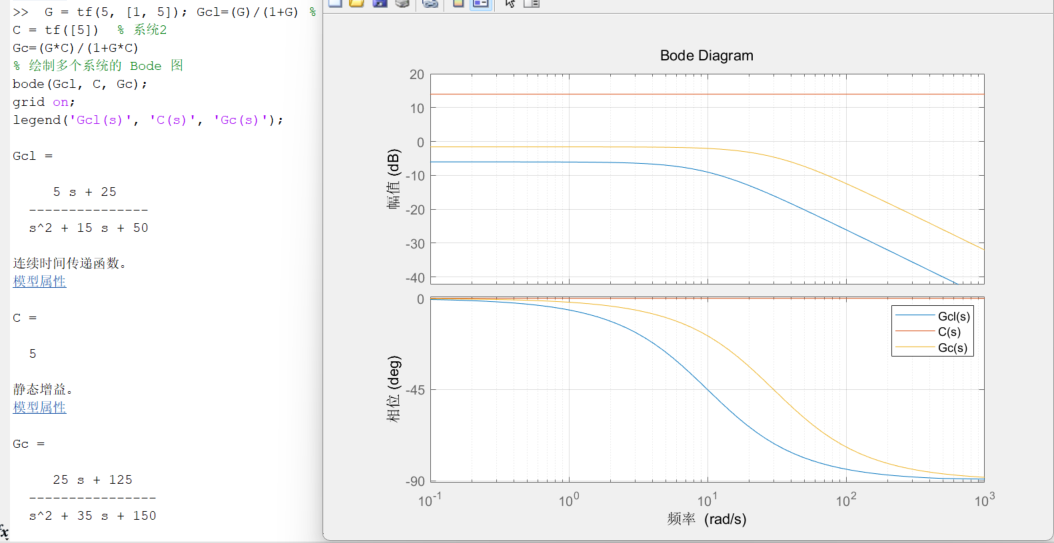
\includegraphics[width=12cm]{picture/C_5.png}\\
        观察伯德图我们可以看到$C(s)=5$,将系统的伯德图整体拉高了,使得稳态误差减少了。\\
        但是我们看到他的抗噪声能力下降了,对比原系统的伯德图,假如输入信号都有一个100Hz的噪声,原系统可以抑制到-20多dB,但是加了只有比例项的PID后只能抑制到-10dB。这个和$C(s)=5$的伯德图本身就有关系(关于伯德图的叠加关系记得看上面dr.can的视频)。所以一旦有这个频段的噪音,系统就会剧烈抖动。\\{\scriptsize 为什么不用考虑低频的噪声,因为噪声普遍是高频的}
      \end{flushleft}
      \vspace{2cm}
      \begin{flushleft}
        所以在比例项的基础上我们会引入积分项,让$K_p=5$,$K_i=1$、$K_d=0$,可得到伯德图如下
        \par 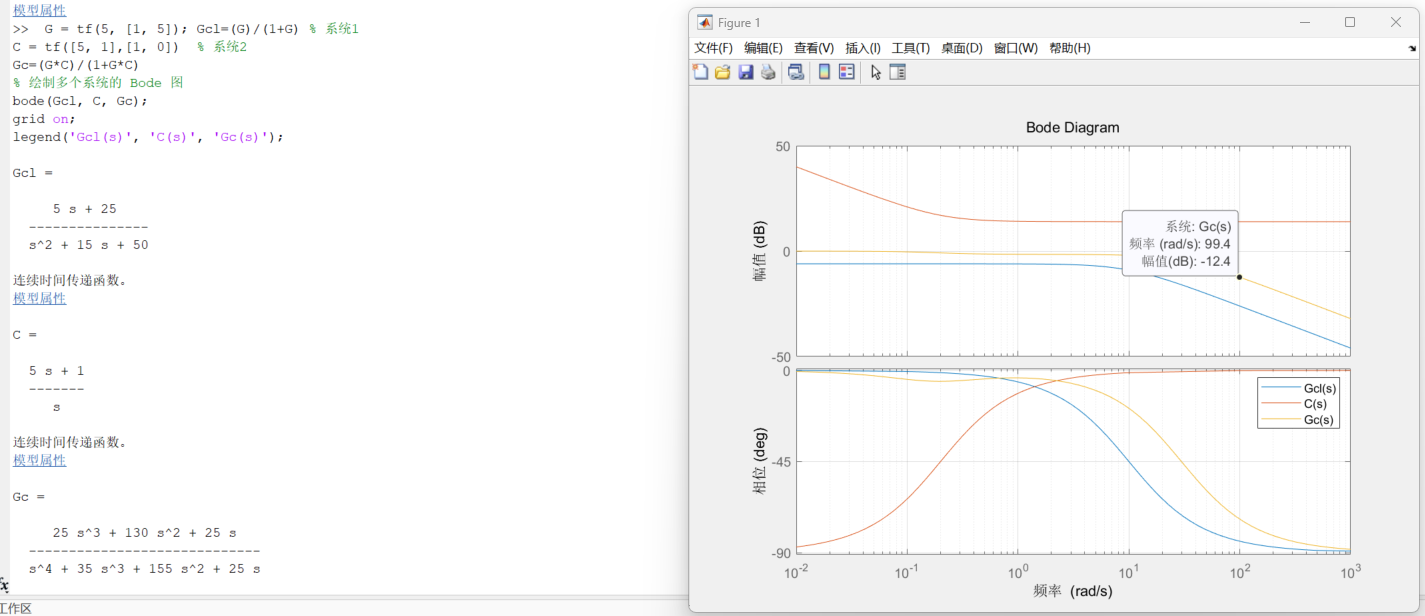
\includegraphics[width=12cm]{picture/C_5_I_1.png}
        \\我们可以看到稳态误差消失了,但是随着频率的升高其幅度响应还是会下降,现在我们的目的就是尽量在不提高噪声对系统的影响下,去提高低频段对0dB的贴合\\
        让$K_p=10$,$K_i=1$、$K_d=0$,伯德图如下,我们可以看到低频段更贴合了
        \par 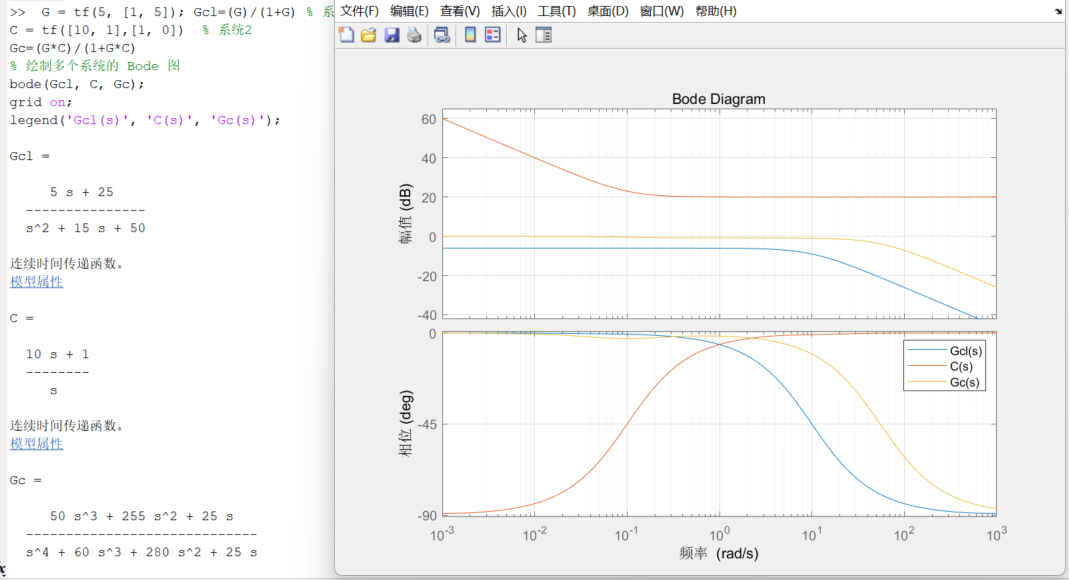
\includegraphics[width=12cm]{picture/C_10_I_1.png}
        \\基本上比例积分控制就可以将系统控制到我们想要的效果。大家可以到matlab去尝试如何改变PID的值才能达到我们的目的
      \end{flushleft}
      

    \end{notitlebox}
    \subsubsection{代码实现}
    按照我们的思路我们需要把我们的输入信号(云台角度参考值)改成可以改变频率的正弦信号,然后我们可以从1rad/s开始,调PID的参数,使输出值能贴近参考值,然后增大频率继续调,大概到10多rad/s就可以了。如果再大的话抗噪声的能力就会下降,系统就容易高频振动,而且我们云台6020电机实际的最大角速度和角加速度也不能达到这么快的响应。 
    \\按照上面的分析随着我们输入的频率不断增大,$K_p $值也要不断地增大,才能让输出跟上输入,当 $K_p $增大到一定的值系统就容易受到噪声干扰而振动。
    \par 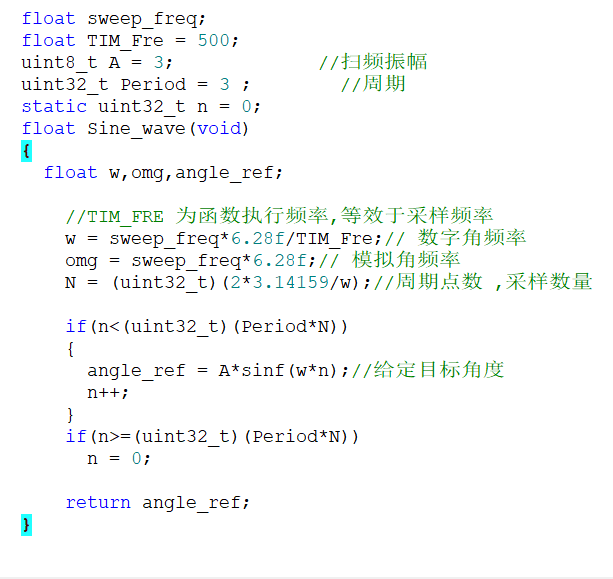
\includegraphics[width=12cm]{picture/code_control_2.png}
    \\普通模式下我们用正弦信号就好了,但是自瞄模式我们需要用锯齿波来进行调参。为什么需要锯齿波呢,是因为在小陀螺的时候我们收到算法的值是一个突变的值,就类似于锯齿波的性质。
    参考代码如下
    \par 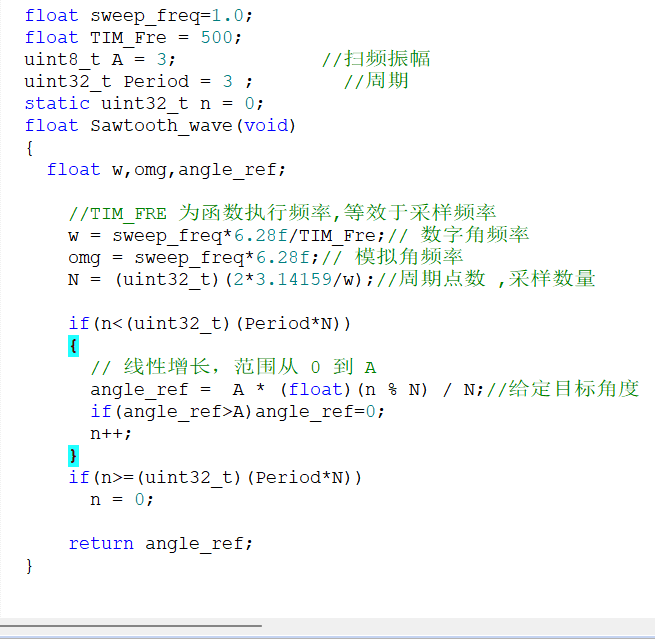
\includegraphics[width=12cm]{picture/code_control.png}
    \\然后跟调正弦波一样调参就行了

    \subsection{前馈控制器}
     \subsubsection{理论知识}
      \begin{titlebox}{什么是前馈控制}
        前馈控制是一种控制策略,没有固定的表达形式。它可以提高系统的响应速度,减小误差,增加带宽但是不改变系统的稳定性。\\
        从字面上来理解就是我们会给系统多输入一个值从而让我们更快的达到目标值。
        \par 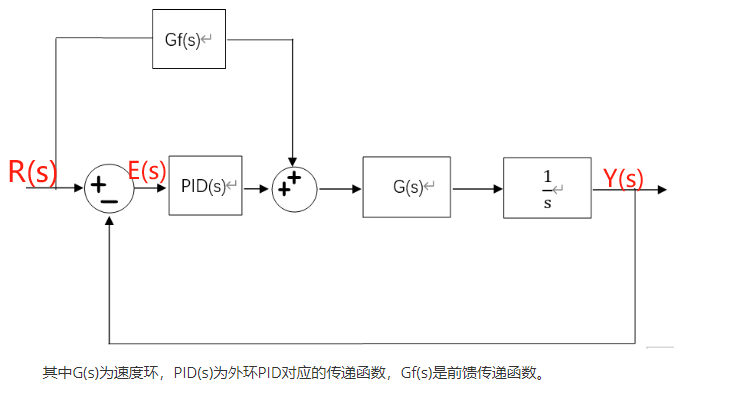
\includegraphics[width=12cm]{picture/FFC.png}
        \\前馈控制有三种基本表现的形式,在这里符合我们需求的是基于受控系统倒数的形式。
        
        下面给大家公式推导来一下(先不用管那个积分器):
        \begin{align*}
         &Y(s)=[R(s)G_f(s)+E(s)C(s)]G(s)\\
         &Y(s)=R(s)G_f(s)G(s)+E(s)C(s)G(s)\\
         &R(s)-E(s)=R(s)G_f(s)G(s)+E(s)C(s)G(s)\\
         &E(s)=\dfrac{1-G_f(s)G(s)}{1+C(s)G(s)}R(s)
        \end{align*}
        另外还可以再推导出整个系统的开环函数:
        \begin{align*}
          \dfrac{Y(s)}{R(s)}=\dfrac{(G_f(s)-C(s))G(s)}{1-C(s)G(s)}
        \end{align*}
        根据我们的推导结果,我们可以看到如果$G_f(s)=\dfrac{1}{G(s)}$,那么在理论上误差$E(s)$就等于0。同时在开环函数中我们可以看到$G_f(s)$改变的是仅是零点,所以可以改变响应的快慢而不影响系统的稳定性。
        
        \href{https://www.bilibili.com/video/BV1Lj421d7Mr/?spm_id_from=333.1387.favlist.content.click&fvd_source=b02f21f21dd17ebeef8dac9338c9d06c}{前馈控制三种形式}

      \end{titlebox}
      \subsubsection{代码实现}
       \textbf{① 速度环的前馈控制}\\
        就用我们上面仿真出来的速度闭环函数:
        \begin{align*}
          G(s)=\dfrac{32.36}{s+33.96}
        \end{align*}
        所以内环的传递函数为
        \begin{align*}
          G_1(s)*\dfrac{1}{s}=\dfrac{32.36}{s^2+33.96s}
        \end{align*}
        
        然后就得到前馈控制的函数: 
        \begin{align*}
           G_f(s)=\dfrac{1}{G_1(s)}=\dfrac{s^2+33.96s}{32.36}
        \end{align*}
        然后根据脉冲不变法就可以得到差分方程了,转换为C语言方程。\\
        \par 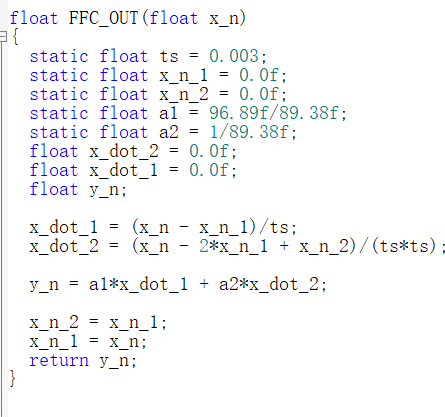
\includegraphics[width=10cm]{picture/FFC_function.png} \\

        下面我给大家推导一下代码中的差分方程怎么来的,这里涉及一些离散信号的知识暂时不懂也没关系,后面有可能就会用到。
        \begin{align*}
          G_f(s)&=\dfrac{s^2+33.96s}{32.36}\\
                &=\dfrac{1}{32.36}s^2+\dfrac{33.96}{32.36}s\\
            g_f(t)&=\mathcal{L}^{-1}{[G_f(s)]}=\dfrac{1}{32.36}\delta''\left( t \right)  + \dfrac{33.96}{32.36} \delta '\left( t \right)\\
            &\text{将信号离散化,$t=nT_s$,$T_s$为采样时间}\\
            g_f(t)&=\dfrac{1}{32.36}\delta''\left(nT_s \right)  + \dfrac{33.96}{32.36} \delta '\left(nT_s\right)\\
            &=\dfrac{1}{32.36}\dfrac{[\delta'(nT_s)-\delta'((n-1)T_s)]}{T_s} +  \dfrac{33.96}{32.36} \dfrac{\delta (nT_s)-\delta((n-1)T_s)}{T_s}\\
            &=\dfrac{1}{32.36}\dfrac{[\delta(nT_s)-\delta((n-1)T_s)-\delta((n-1)T_s)-\delta((n-2)T_s)]}{T_s^2} \\&+  \dfrac{33.96}{32.36} \dfrac{\delta (nT_s)-\delta((n-1)T_s)}{T_s}\\
            &=\dfrac{1}{32.36}\dfrac{[\delta(nT_s)-2\delta((n-1)T_s)-\delta((n-2)T_s)]}{T_s^2} +  \dfrac{33.96}{32.36} \dfrac{\delta (nT_s)-\delta((n-1)T_s)}{T_s}
        \end{align*}
        最后转换成差分方程,设输入信号为$x(n)$,输出信号为$y(n)$
        \begin{align*}
          \dfrac{1}{32.36}\dfrac{[x(nT_s)-2(x(n-1)T_s)-(x(n-2)T_s)]}{T_s^2} +  \dfrac{33.96}{32.36} \dfrac{x((n)T_s)-x((n-1)T_s)}{T_s}
        \end{align*} 
        我们的代码里面$x_n$的参数已经是根据采样时间得到的,因为我们的采样时间是按照freertos执行的频率来算的,当我们的代码执行到这里的时候也就是0.003s了,这就是为什么代码里面不需要再对$x_n$进行处理
        \begin{flushleft}
          写完函数之后我们就可以直接用了,
          \par 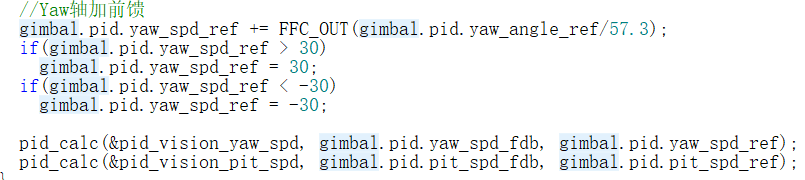
\includegraphics[width=12cm]{picture/FFC_code.png}
        \end{flushleft}
        \begin{flushleft}
          在我们的代码里面我们的“angle\_ref”的单位是度,而我们建模的单位是弧度(rad),所以我们需要进行角度的转换才能代入函数,而且由于电机的物理特性限制我们最大的角速度是$\pm 30$,所以我们需要进行一个限幅(这些都可以通过查手册、计算知道的)
        \end{flushleft}
        \textbf{② 电流环的前馈控制}\\
        上面我们学习了速度环的前馈控制,接下来我们学习一下电流环的前馈控制。至于为什么我们学习了速度环的控制还要再学电流环的控制呢?虽然在普通模式下用速度前馈的是非常流畅且静态误差很少,但是在进入自瞄的情况下云台会出现非常严重的超调现象。这是因为算法发给我们的自瞄值是一个突变的值,而且还带有比较严重的噪声信号,所以导致云台在自瞄的时候会出现非常大的超调现象。\\
        而电流前馈控制可以有效的解决这样状况,因为电流前馈是直接作用于电压指令(PWM调制前),补偿电气的 L/R 时间常数(通常微秒级)。电流环带宽可提升至1kHz~10kHz,适合高频扰动抑制。再加上电流前馈对于PID参数的敏感度更低

        \subsection{阻力扭矩补偿}
          \subsubsection{理论知识}
          \begin{titlebox}{怎么理解阻力扭矩补偿}
            首先,我们需要先知道我们为什么需要阻力扭矩补偿?\\
            考虑到物理现实的原因,我们云台转轴相关连接件之间是有摩擦阻力的这是无法避免的。
            所以,我们电机时间的云台转角和输入力矩之间的真实关系并不是如上面的模型所说的那样理想,其真实的物理模型应当如下:
            \begin{align*}
              J\overset{..}{\theta}+b\overset{.}{\theta}+N=T
           \end{align*}
           其中,b为粘滞摩擦系数(可以简单的理解为和我们上面说的阻尼系数是一样的),N为动摩擦或静摩擦力矩(即阻力扭矩)
           \\这里我们可以看到,由于静摩擦或动摩擦力矩的出现,模型引入了非线性量$N$,通过我们前面的PID的学习我们可以知道,PID对非线性时不变系统的处理是比较差的。
           
           \begin{flushleft}
              为什么对非线性的处理会比较差呢?在这里我略加解释一下,有利于大家理解,以我们控制的电机为例:
              \\\textbf{对于比例项P来说,}非线性会导致增益 $K_p$的有效性变化
            \begin{itemize} 
              \item 在低速时,静摩擦占主导,需要更大的$K_p$才能克服。
              \item 而在高速时,动摩擦$+$粘滞摩擦占主导, $K_p$需求降低。
            \end{itemize}
           \end{flushleft}
          \begin{flushleft}
            在控制系统调试过程中,由于参数整定的局限性,$K_p$的可调范围受到约束。具体表现为:在低速工况下整定的$K_p$ 值,若直接应用于高速工况,可能导致系统失稳甚至发散(如出现显著的超调或振荡)。这一现象凸显了系统动态响应(如快速性)与稳定性(如超调抑制)之间的固有矛盾,本质上是由于系统在不同工作点下的动态特性(如带宽、相位裕度)随工况变化而导致的鲁棒性不足问题。
          \end{flushleft}
           \begin{flushleft}
            \textbf{对于积分项I来说,}非线性会导致积分饱和(Integral Windup)或稳态误差波动。
            \begin{itemize} 
              \item 齿槽效应导致扭矩周期性波动$\rightarrow$ 积分器持续累积误差,引发振荡。
              \item 静摩擦导致“死区”,积分器需要更长时间补偿。
            \end{itemize}
           \end{flushleft}
           \begin{flushleft}
            {\scriptsize 下面我会结合传递函数的知识给大家讲解一下,有助于大家理解,如果还看不懂的话那就记住上面的结论吧。\\
            先将上面的微分方程进行拉普拉斯变换,得到:
            \begin{align*}
              &Js^2\varTheta \left( s \right) +bs\varTheta \left( s \right) +\dfrac{N}{s}=T\left( s \right) \\
              \Rightarrow&\varTheta \left( s \right) =\dfrac{T\left( s \right)}{Js^2+bs}-\dfrac{N}{s\left( Js^2+bs \right)}\\
            \end{align*} 
            前面一项是我们理想的系统,后面一项是非线性项(扰动项)。而这个非线性项就是我们需要补偿的阻力扭矩。\\
            }
           \end{flushleft}
           \begin{flushleft}
            这个阻力扭矩在我们小陀螺的时候会尤其明显,在和算法联调的时候可以发现我们离目标会有一个稳定的偏角,所以我们需要对阻力扭矩进行补偿,来消除非线性项对系统的影响,即消除动摩擦或者静摩擦的影响。至于为什么不用积分,我相信我上面已经说清楚了。
            \\说白了其实这个阻力扭矩补偿也是一种前馈控制器,是我们对已知的量进行补偿,这个请参考我上面让大家看的前馈控制三种形式。
           \end{flushleft}
           
           
          \end{titlebox}
          这里可参考中科大的\href {https://www.bilibili.com/video/BV1xJo4YPEuS?spm_id_from=333.788.videopod.sectionsvd_source=b02f21f21dd17ebeef8dac9338c9d06c}{阻力扭矩补偿}的视频
          \subsubsection{代码实现}
          \begin{flushleft}
            首先我们应该怎么获取这个阻力扭矩呢?我们可以通过实验的方法来获取该值,我们让云台的yaw轴缓慢匀速的转动,缓慢的目的是忽略粘滞摩擦力的影响,而匀速的目的是让云台的动力和阻力二力平衡从而间接获得阻力扭矩。\\
            
          \end{flushleft}
          \begin{flushleft}
            OK,理论成立,我们就要知道怎么去实现。\\
            我们可以通过vofa+来采样匀速转动的电流值,为什么是电流值呢?因为电流值和力矩是成正比的,电流越大,力矩越大。至于怎么让他匀速转动,我相信能看懂这个文档的学弟学妹应该不需要我教了,这里我就不赘述了。\\
            \textit{这里需要注意一下,对于6020来说有两种控制电机的方式:电流控制和电压控制。如果是电压控制的话,这个补偿的效果不会很好,因为电压和力矩不是线性关系。6020如果是电压控制的话就刷一下固件,如果是4310的达秒电机则无所谓,因为4310只有电流控制}
          \end{flushleft} 
          
        \begin{flushleft}
          以哨兵的云台为例,哨兵云台的yaw轴是4310的达秒电机,我们让他以转速为1.4rad/s进行旋转。然后,对其电机的电流进行采样。得到如下图所示的波形。(提醒一下采样前记得把底盘注释掉)
           \par 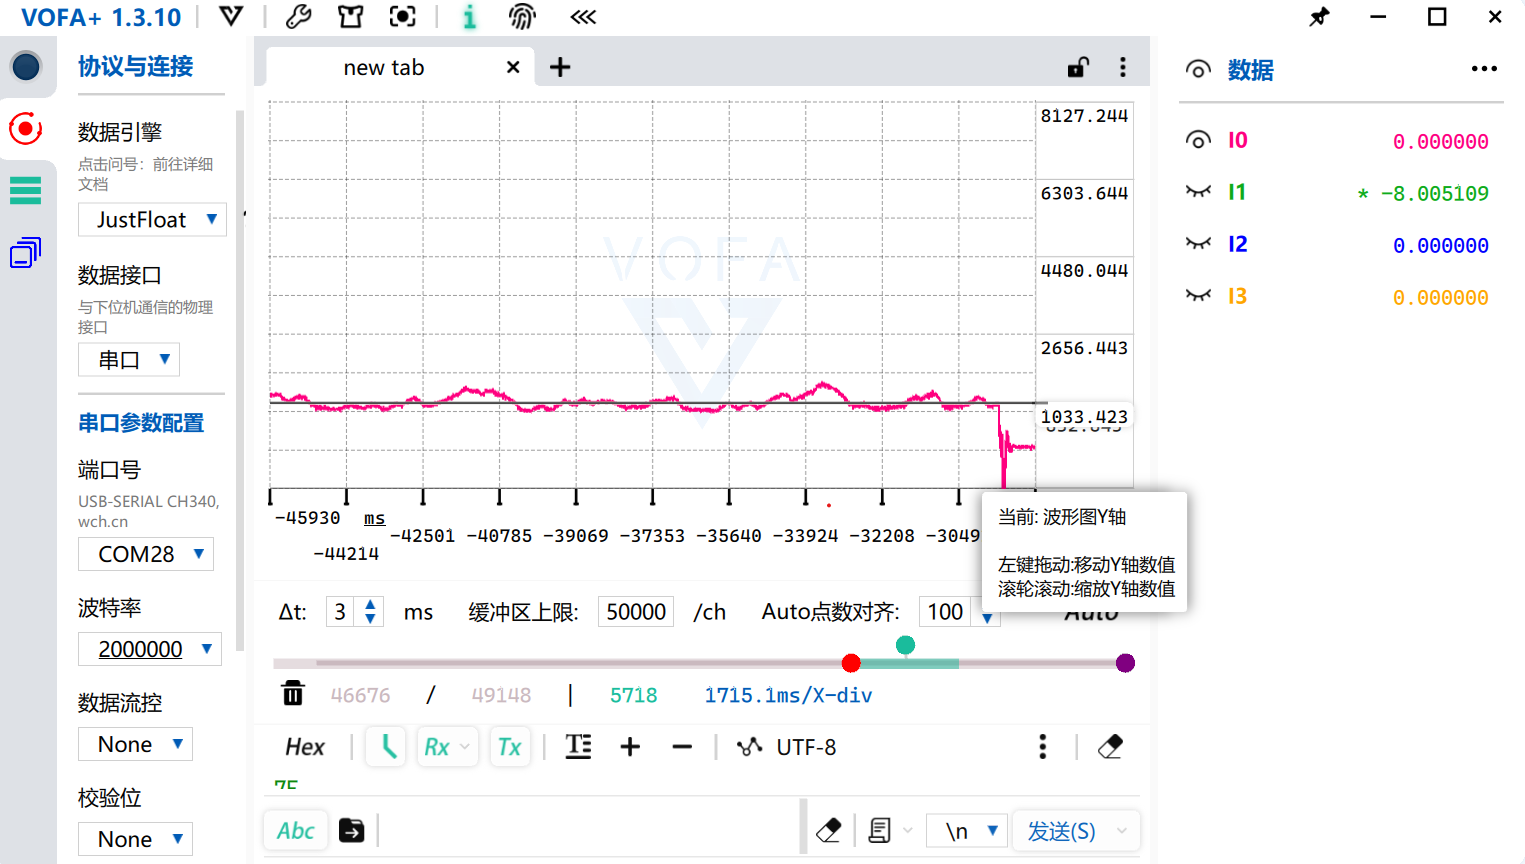
\includegraphics[width=12cm]{picture/yaw_current_compensation.png}\\
             {\scriptsize 这里可以看到我们的电流曲线并不是一条完美的直线,首先就是因为我们电机的电流采样是有噪声的,其次就是因为我们电机的转速并不是一个完美的匀速转动,我们需要进过PID的闭环运算,所以无法达到绝对的匀速,所以我们得到的曲线并不是一条完美的直线。
            }
        \end{flushleft}
        
        \begin{flushleft}
          我们只需要取它的平均值,这个平均值可以不用太准确,对于现在的波形图来说,他的平均值就是1050左右
        \end{flushleft}
          所以我们可以得到一个低配版的转速和阻力扭矩的关系(要时刻记住直流无刷电机电流和力矩是成正比的),这个函数图是一个非常理想的图,它忽略了静摩擦的影响,直接简化为一个阶跃函数,对于电压控制的电机可以这样粗糙的给补偿:
          \par 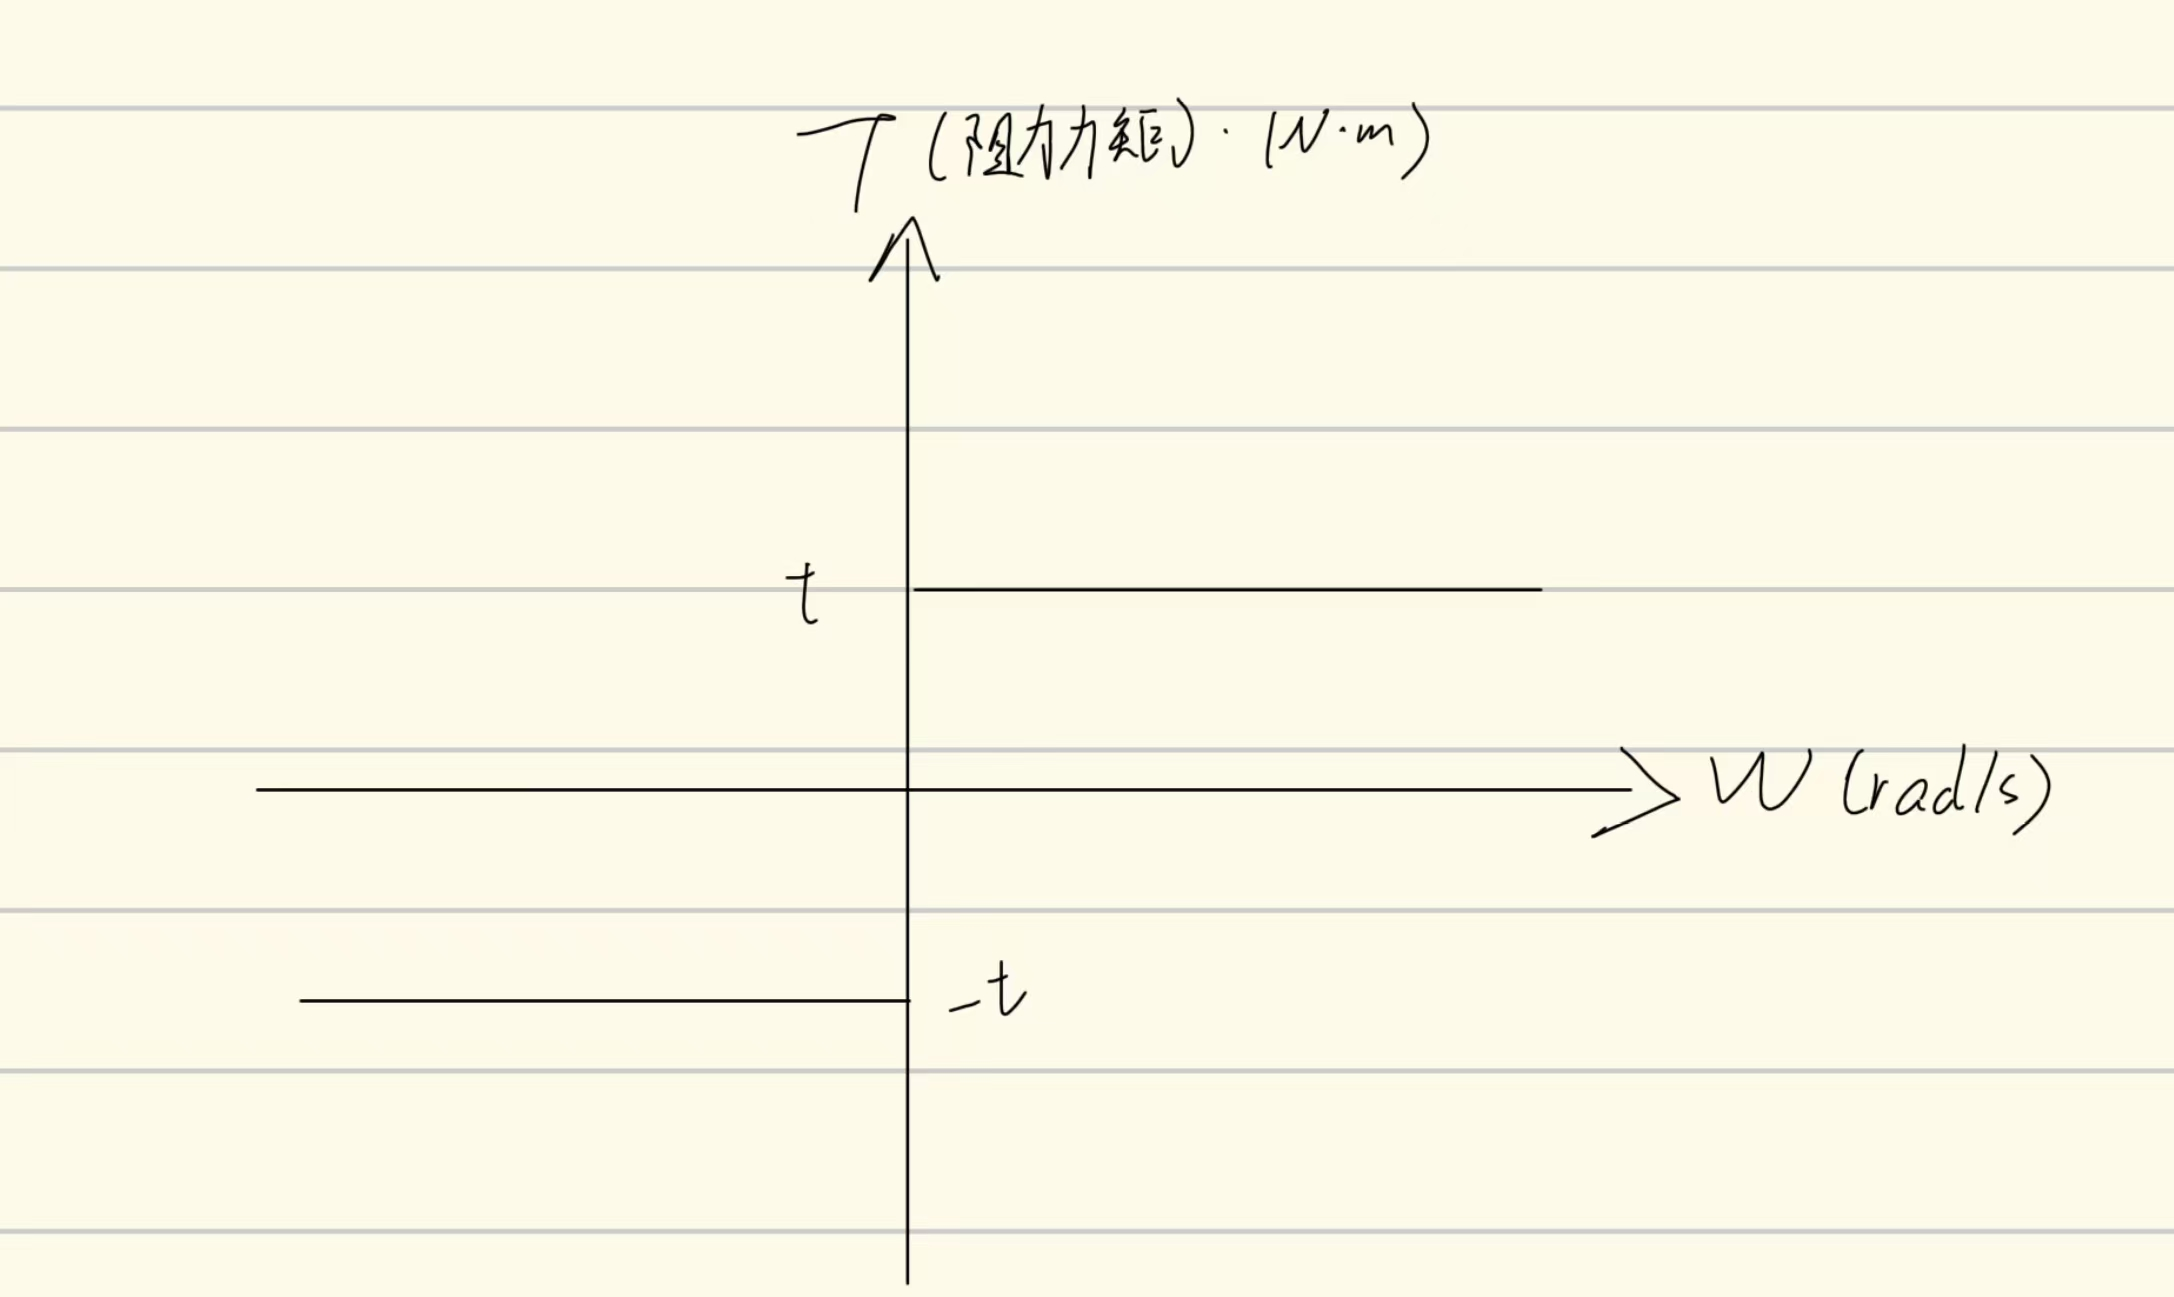
\includegraphics[width=12cm]{picture/yaw_compensation.png}
        \begin{flushleft}
         但是在这个低配版的阻力扭矩补偿中,假如我们的值处于零点附近的话,那么就可能出现零点震荡的现象,这是因为倘若转速在零点附近波动时,我们会发现电流值会在1050和-1050之间来回波动,这个时候电机就会容易抽搐,所以我们需要对这个函数进行一个平滑处理,才能得到一个比较理想的函数图。\\
         至于如何处理:我们可以将零点附近的一小段区间用正比例函数贴合过去,称之为“一阶连续化”。
         \par 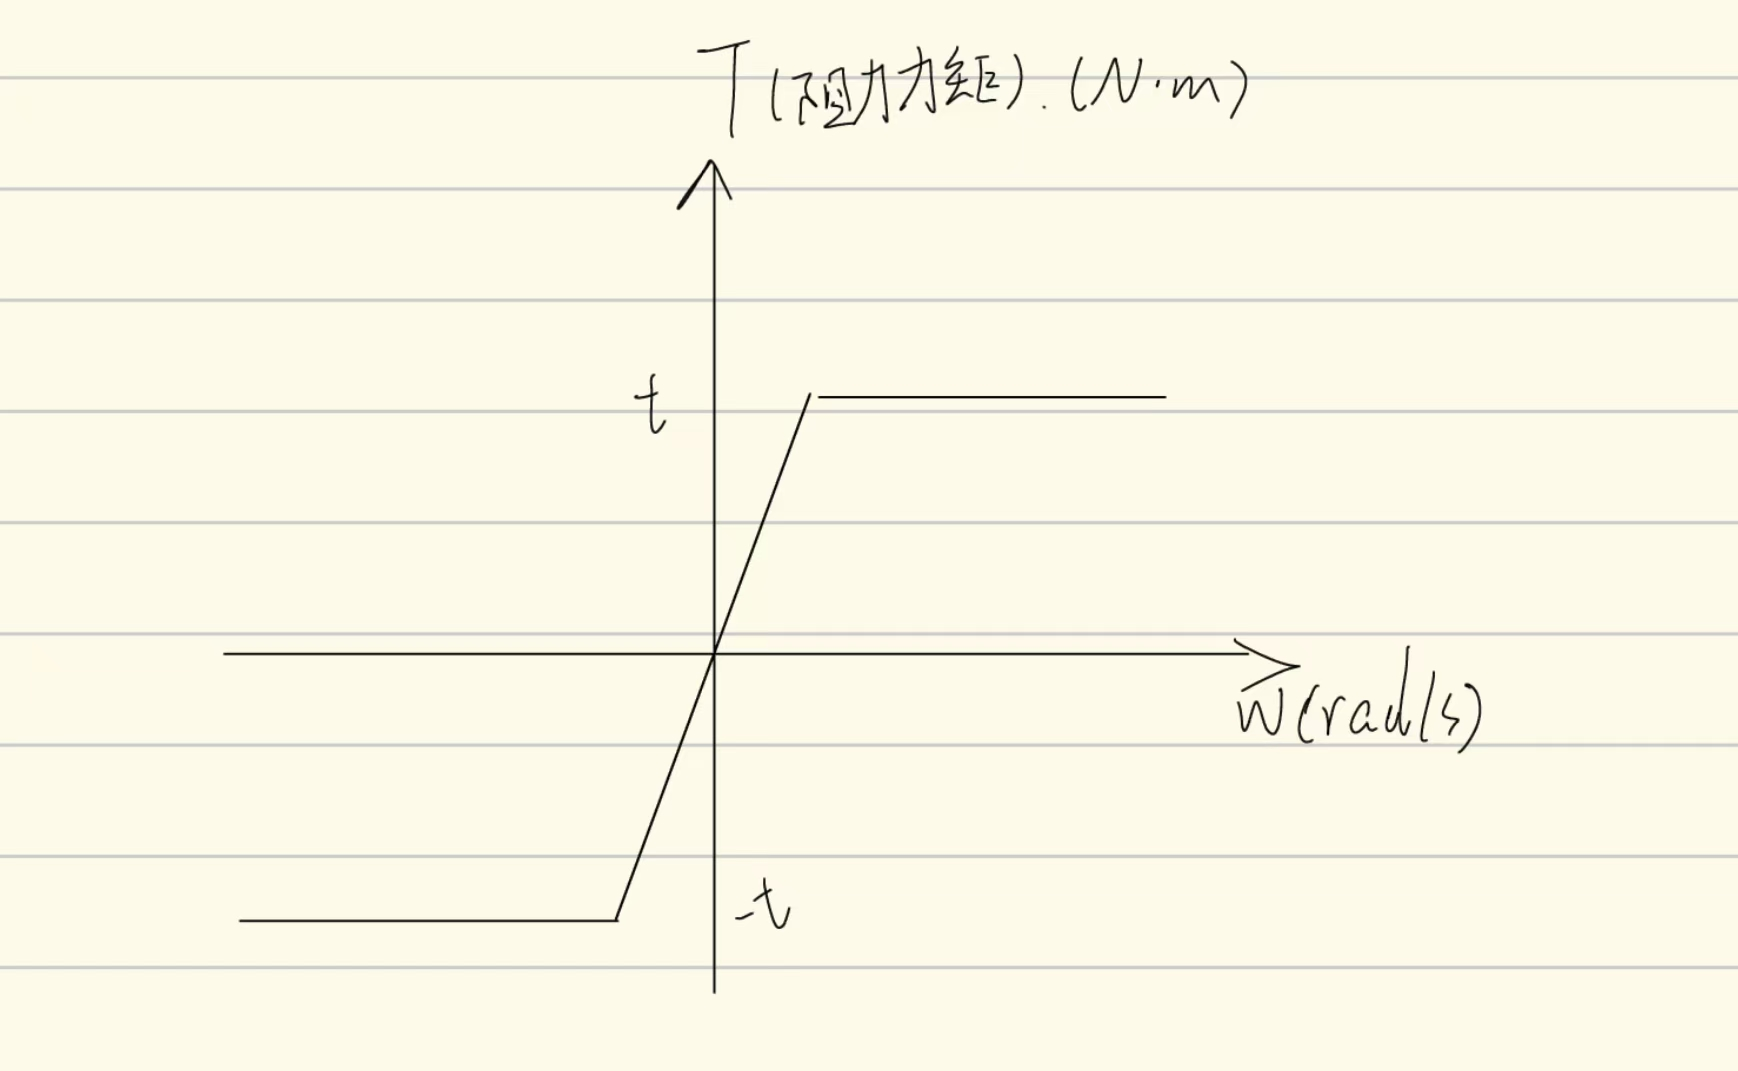
\includegraphics[width=12cm]{picture/linearization_yaw.png}\\
         按照上面的函数图我们就可以写出以下的代码,实现这个函数的功能。(注意这是电流补偿,所以是直接加到你要发送的电流上)\\
         \par 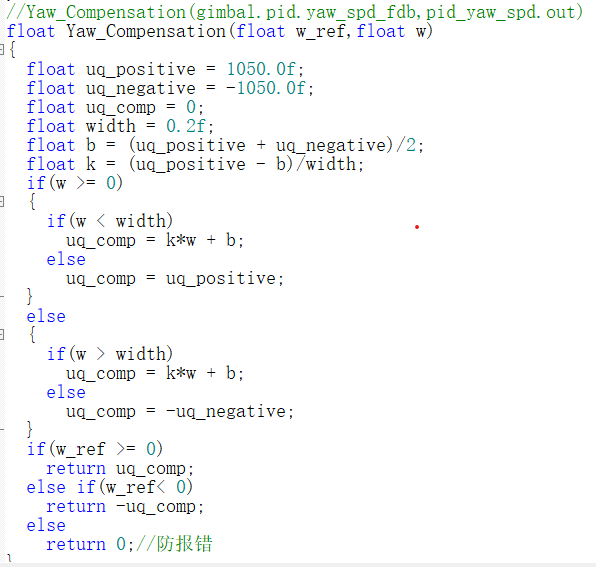
\includegraphics[width=12cm]{picture/yaw_compensation_code.png}\\
        \end{flushleft}
       
        \subsection{参考输入微分的前馈补偿}
        \subsubsection{理论知识}
        \begin{titlebox}{什么是参考输入微分的前馈补偿}
          {
             \hspace{1cm} 大家有可能会在代码中看到这个函数float getFeedforwardControl,也有可能已经被删了,但是不管怎么样我这里也顺便说一下。但是我们一般不使用这个前馈方式,所以我也就稍微讲一下理论知识,也把前馈的最后一种形式说一下,让文档更完整一点  \\ 
            \hspace{1cm}  参考输入微分的前馈补偿是指在控制系统中,直接对参考输入信号进行微分处理,以便更好地预测和补偿系统的动态响应。其主要目的是通过提前计算出系统对参考输入的响应,从而提高系统的跟踪性能和响应速度。\\
            我们从最开始的微分方程开始推导:\\
            \begin{align*}
              J\overset{..}{\theta}+b\overset{.}{\theta}=T
           \end{align*}
            将其差分离散,让我们可以用代码来实现:
          \begin{align*}
              &J\left(\dfrac{\theta(n+1)-2\theta(n)+\theta(n-1)}{T_s^2}\right)+b\left(\dfrac{\theta(n+1)-\theta(n)}{T_s}\right)=T(n) \\
              \Rightarrow&\dfrac{J}{T_s^2}[\theta(n+1)-2\theta(n)+\theta(n-1)]+\dfrac{b}{T_s}[\theta(n+1)-\theta(n)]=T(n)
            \end{align*} 

            其实上面可以理解为,在知道精确的系统的微分方程时,用几个输入的离散点来对输出进行一个短时预测。\\
            假如我们需要将在位置环中加入前馈,就需要用第一项来进行补偿,如果在速度环中加入前馈则需要用到第二项进行补偿\\
          
            但是这个控制器的实现我们需要考虑两个问题:\\①我们的转动惯量J和阻尼系数b并没有办法知道,即使云台的转动惯量可以问机械拿到(其实SolidWorks也并不准确,但是只是作为一个前馈控制器的参数也勉强可以用),但是阻尼系数b是无法知道的。这时可能会有读者问为什么不可以用上面的仿真出来的系统函数来反推转动惯量和阻尼系数呢?这个就关乎于我们的第二个问题了。\\
            ②我们曾经说过,我们可以简单的将的电机输出力矩可以看做与输出电流成正比的关系,即$T=K_tI$,其中$K_t$为电机的力矩常数。我们的输入和输出都是电流值,所以说我们仿真出来的系统函数与实际的系统函数其实是还差一个$K_t$值即:\\
            \begin{align*}
            & JsW(s)+bW(s)= K_tI(s)\\
           \Rightarrow&G(s)=\dfrac{K_t}{Js+b}
            \end{align*} 
            这个$K_t$值我们暂时没有办法得出来,即使得出来了最后的效果也不一定好,因为我们只是理想的认为力矩电流和力矩是成正比的,其实其中还有非线性因素存在。\\

            \textit{以上的问题基于我现在水平和能力暂时没有办法解决,由于无法实操其理论知识依然停留在表层,有兴趣的学弟学妹可以尝试去解决一下,或者有更好的方法也可以告诉我,我会在文档中进行更新。}\\
          }

        \end{titlebox}
        \begin{notitlebox}
        \textit{讲到这里我小小的提一嘴,其实前馈的三种形式我们已经全部学完了,并且能很好的融入到我们的代码之中,还有不理解的可以再次参考一下我上面推荐的前馈控制的三种形式的视频再回头看看文档,希望大家有更深刻的理解。}          
        \end{notitlebox}
        \subsection{重力补偿}
      
      
        \subsection{低通滤波器}
      
      
      
        \subsection{跟踪微分器}
        \begin{flushleft}
          为什么我会讲解这个控制器呢?因为在我之前使用键鼠调车的时候发现我鼠标输入的值变成了阶跃信号,而非一条平滑的曲线,这导致了我的云台一卡一卡的。后面有师兄帮我加了这个控制器之后曲线就变得平滑了。
          \\为了防止大家后面也遇到这种情况,这里给大家讲解它的用法,除了平滑曲线之外它还可以抑制超调现象,在一定情况下可以使用。
        \end{flushleft}
          \subsubsection{理论知识}
          
           \begin{titlebox}{什么是跟踪微分器}
            \begin{flushleft}
              跟踪微分器主要用于从含噪声的输入信号中提取跟踪信号及其无噪声的微分信号,同时安排过渡过程避免系统超调。其核心设计思想是“通过动态过程生成平滑的过渡轨迹,而非直接使用跳变的输入信号。
              
            \end{flushleft}
          \end{titlebox}
          \begin{flushleft}
            跟踪微分器的传递函数为:
            \begin{align*}
             G(s) = \dfrac{r^{2}}{s^2+2rs+r^{2}}
            \end{align*}
            观察发现,其实它是由我们上面推出来过的二阶系统通用系统响应$G(s)=\dfrac{\omega _{n}^{2}}{s^2+2\xi \omega _ns+\omega _{n}^{2}}$,然后令$\xi=1$得到的\\
              
            
            这是一个临界阻尼系统,我们为什么要用它来作为我们的跟踪微分器的系统呢?
            \\这是因为跟踪微分器需要满足生成平滑过渡轨迹并提取微分信号的目标,需要无超调,且快速反应。
            如果是欠阻尼($0<\xi<1$)则会存在超调、震荡,如果是过阻尼($\xi>1$)的话,过渡时间随$\xi$增大显著延长,所以说临界阻尼系统是阶跃响应不产生超调的前提下衰减速度最快的系统。
            \par 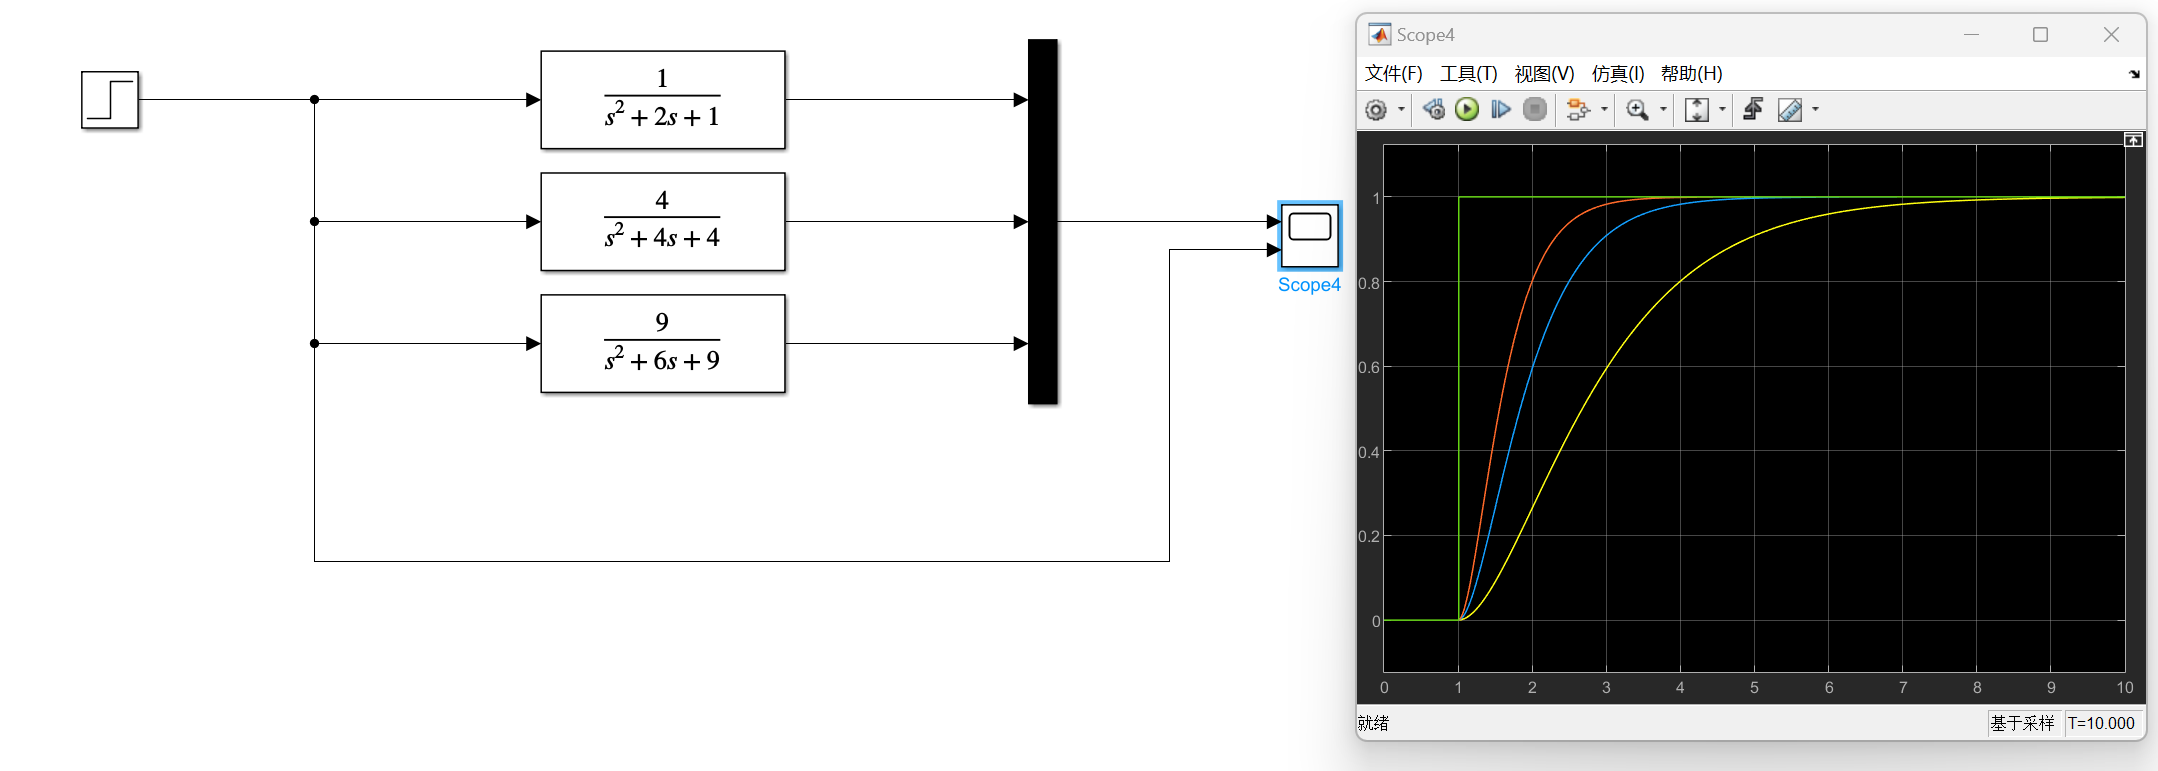
\includegraphics[width=12cm]{picture/tracking_differentiator.png}\\
            通过上面的图我们看出,跟踪微分器将一个阶跃信号转化为一条平滑的曲线,并且随着我们的r变大,信号跟踪的速度也会越快。这样我们的目的就达到了,将突变的信号转换为平滑的曲线

          \end{flushleft}
             \begin{flushleft}
              
            \par 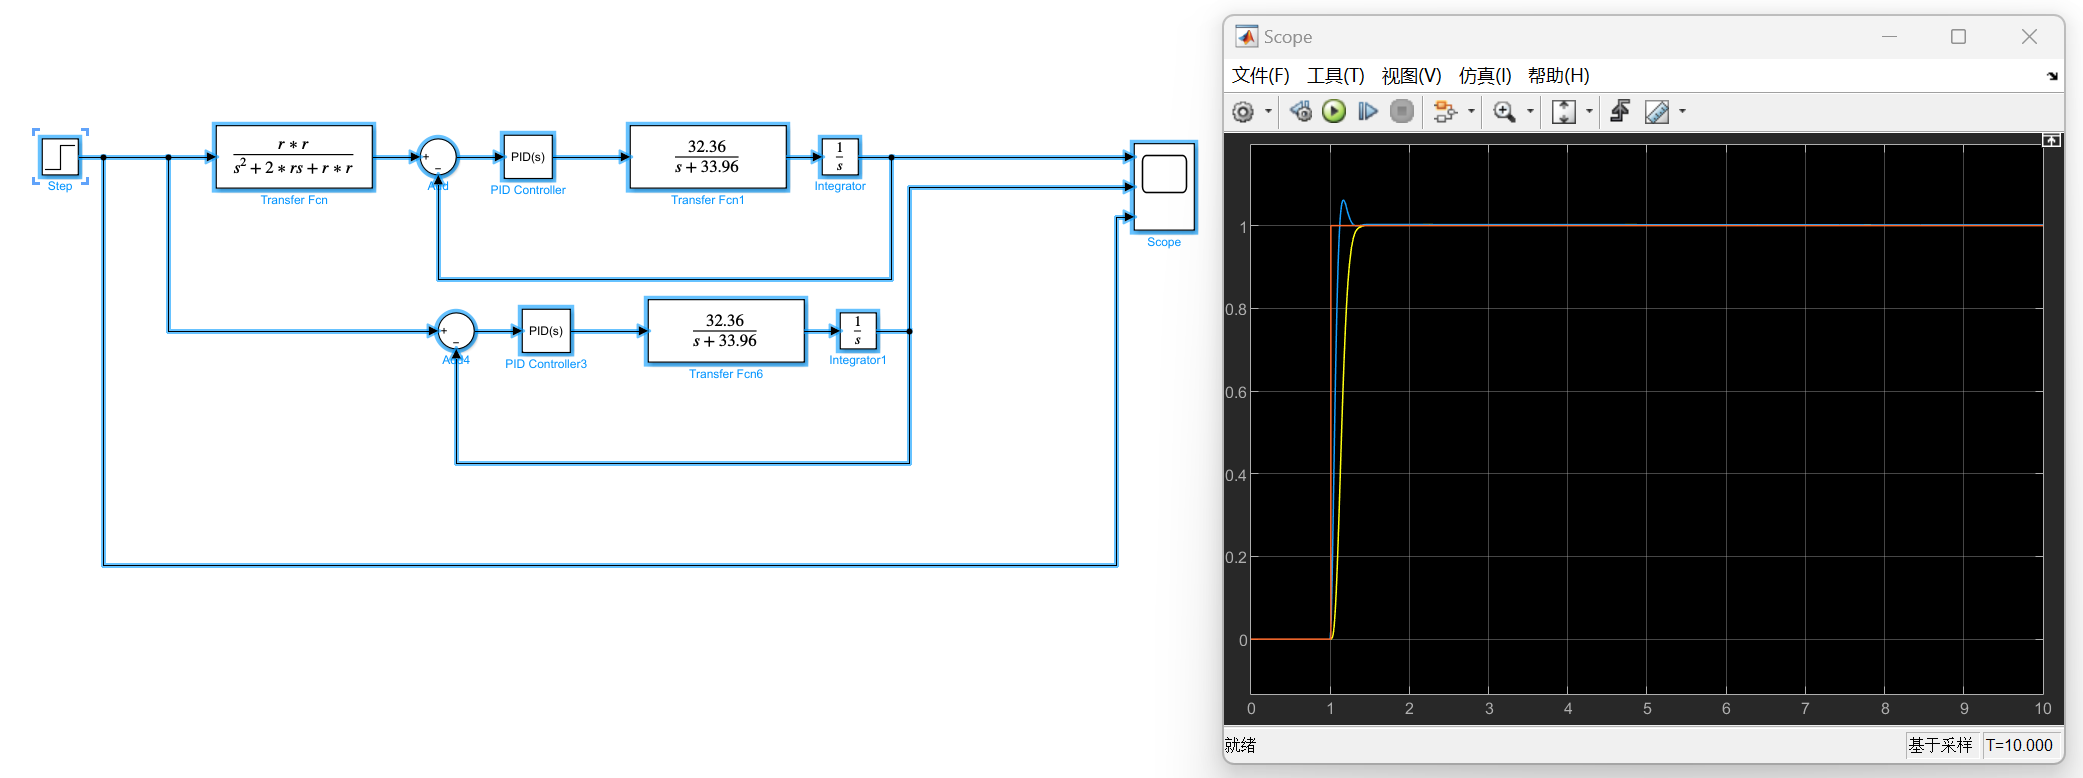
\includegraphics[width=12cm]{picture/tracking_differentiator_pid.png}\\
            从传递函数的角度来看,结合PID控制器我们可以得到如上的控制框图(图中r=20,PID系数相同),我们的输入信号被跟踪微分器变平滑之后超调的部分就消失了。
            \end{flushleft}
            还有一个问题就是我们为什么要让曲线变得平滑?这里我引用别人的解释
            \begin{notitlebox}
              
              \begin{quotation}
                我们首先从物理上直观地去认识。不考虑偏载力矩、摩擦力矩等非线性因素,现假设某云台的最大加速的加速度和最大减速的加速度相同,记作$ a_{max}$,现在想要其以最快速度不超调的向某个方向转动 $x$ 度,我们应该怎么做?根据高中物理,我们知道,应该先让云台以 $a_{max}$的加速度加速到 $\dfrac{x}{2}$处,然后再让云台以$a_{max}$的加速度减速运动到 $x$。这就是一个简单的三角规划,它蕴涵了时间最优控制的思想。
                \\\indent 那我们如果直接使用 PID,令这个云台去响应一个阶跃信号会发生什么呢?阶跃信号是一个物理系统无法实现的信号,当执行器性能远超于负载时(即相较于负载惯量和偏载力矩而言,电机输出的电磁转矩非常大,且额定转速满足系统快速性的要求),我们会发现,系统响应阶跃信号也可以响应的很好。
                \\\indent 但大部分物理系统的执行器性能都是和实际需求相匹配的,在这种情况下,如果我们想要快速性,令云台刚开始以 $a_{max}$的加速度加速,不管怎么调 PID 的参数,其在$\dfrac{x}{2}$ 至 $x$ 的区间内 ,一定无法一直以 $a_{max}$的加速度减速,那么就会产生超调。如果我们不想要超调,那刚开始就一定只能用比较小的加速度来加速。这就是传统 PID “快速性”和“超调”之间的矛盾。
                \\ \indent 所以我们需要对输入信号进行处理,使之变得物理可实现
              \end{quotation}
            
            \end{notitlebox}
             \begin{flushleft}
              最后一段话可以这么理解:如果一开始就以 $a_{max}$的加速度加速,在$\dfrac{x}{2}$的时候就无法直接以 $a_{max}$减速,因为加速度从$a_{max}$到$-a_{max}$是需要时间的。那么在加速阶段,云台以$a_{max}$加速,积累了较大的动能。在减速阶段,如果无法一直以 $a_{max}$减速,意味着系统无法在相同的时间内消耗完这些动能,动能转化为运动,导致云台继续向前运动,直到动能被完全消耗,这就是超调的表现。
             \end{flushleft}

            \begin{flushleft}
              看到这的话,你对跟踪微分器有了一个表层的理解了,下面我会从现代控制的角度去讲解跟踪微分器,虽然现控不在本文档的范围内,但为了大家可以更深刻的理解,我会从这个角度给大家解释,大家只需要懂个大概就行。
            \end{flushleft}
            
            
              由传递函数可以得到其状态空间方程:
            $$ 
            \begin{cases}
              \overset{\cdot}{v}_1=v_2\\
              \overset{\cdot}{v}_2=-2rv_2-r^2\left( v_1-v_0 \right) 
            \end{cases}$$
            $v_0$---目标信号;$v_1$---过渡目标;$v_1$---过渡目标微分;$r$---决定跟踪快慢的跟踪因子
            \begin{flushleft}
              由状态空间方程可以得到微分控制器的框图,可以简单的等效为上面所说的跟踪微分器的系统传递函数
              \par 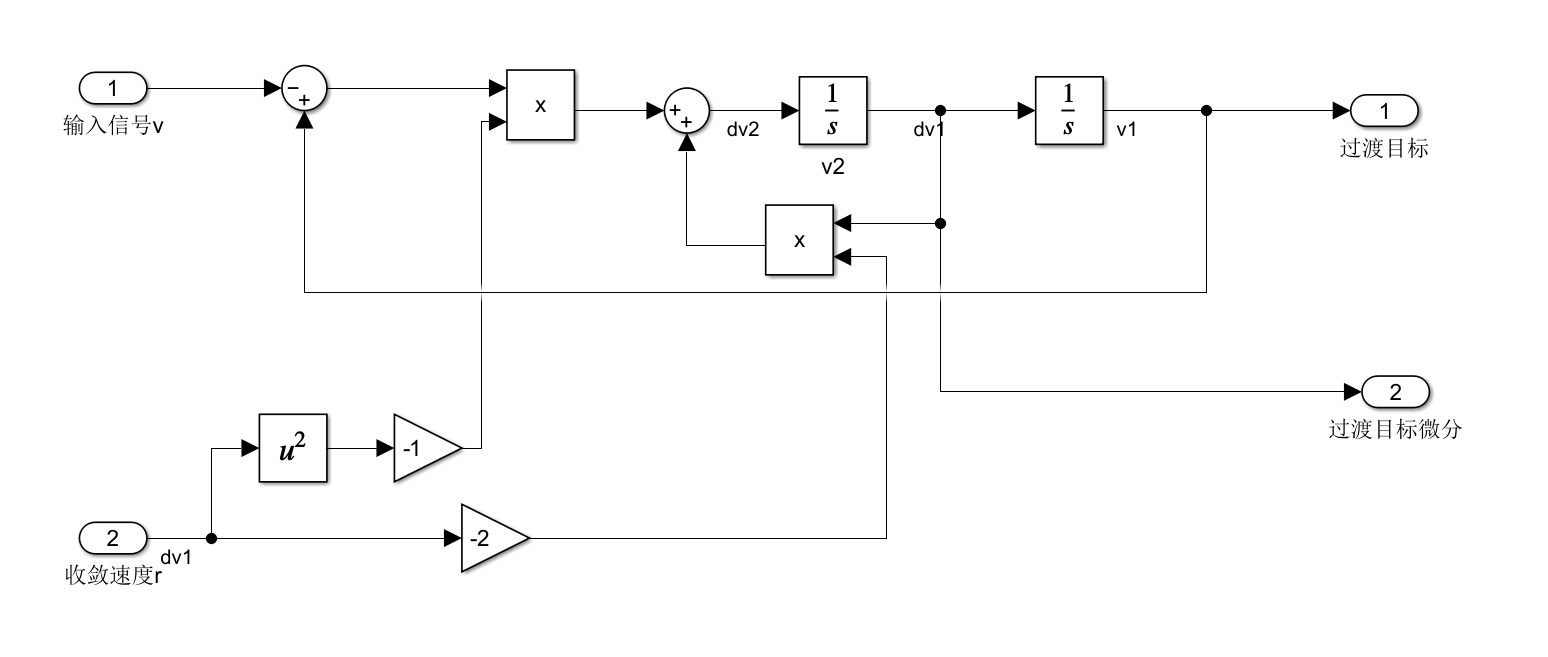
\includegraphics[width=12cm]{picture/tracking_differentiator_ss.png}\\
              为了让读者对控制流程有清晰的认识,下面是整个控制的框图
              \par 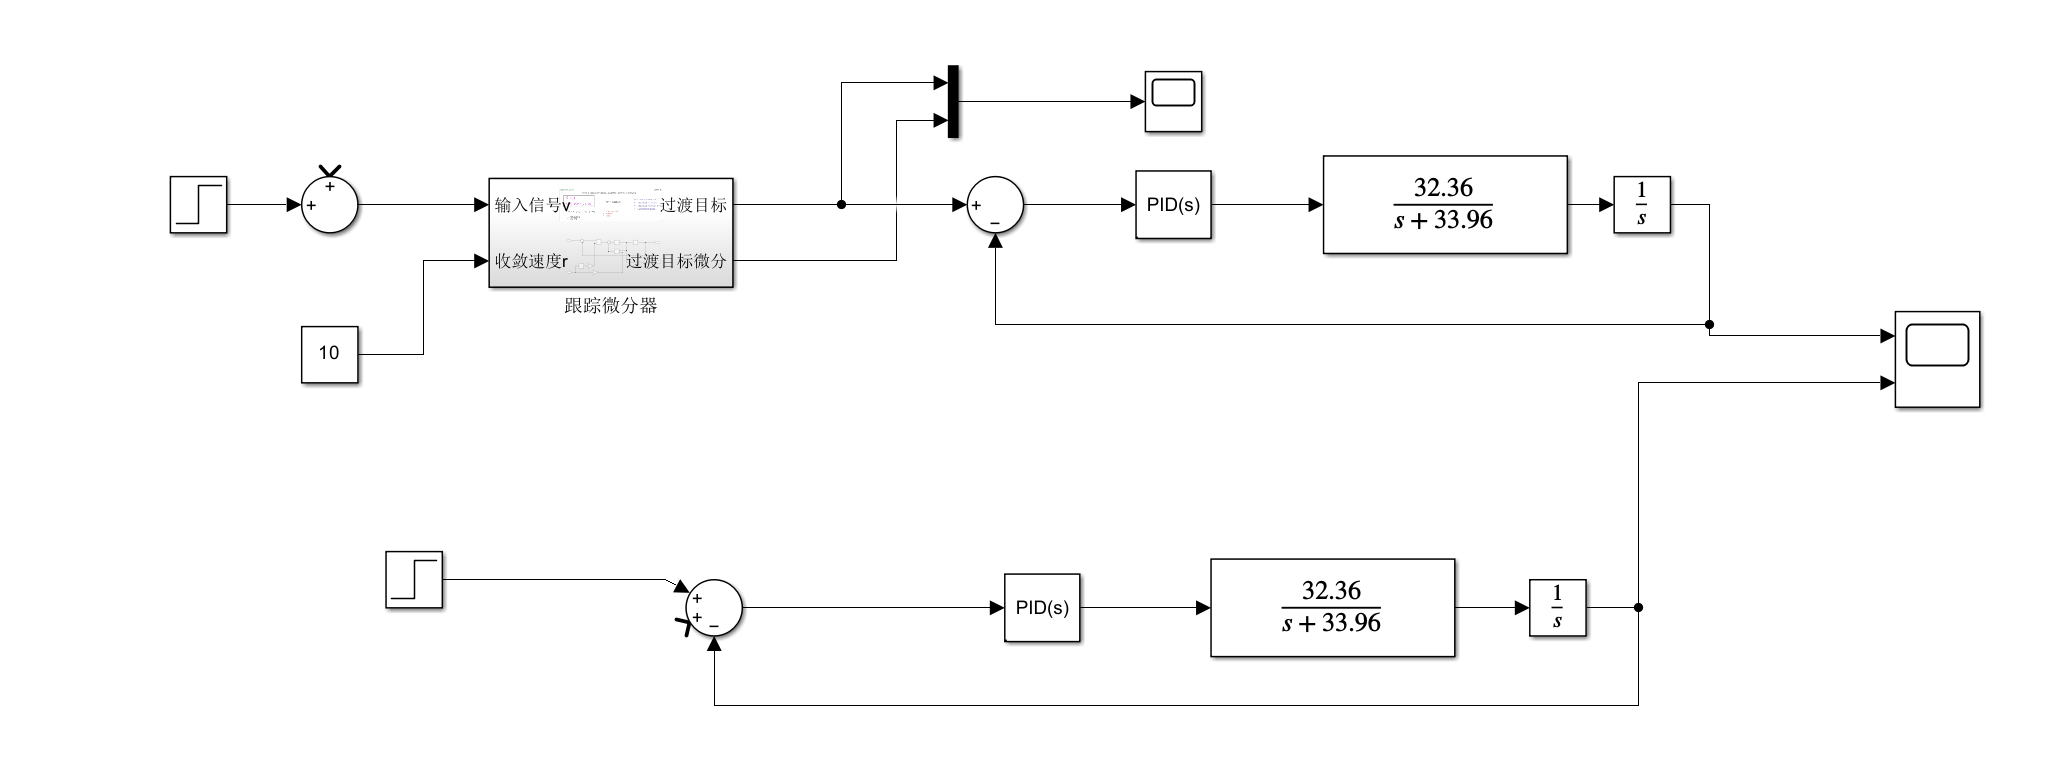
\includegraphics[width=12cm]{picture/tracking_differentiator_ss_all.png}\\
              \end{flushleft}
              跟踪微分的核心机制:\\
              (1)误差反馈\\
              误差项$e=v_1-v_0$,直接驱动系统的状态变量$v_2$\\
              把$e=v_1-v_0$代入状态空间方程:
              \begin{align*}
                \overset{\cdot}{v}_2=-2rv_2-r^2e
              \end{align*}
              \begin{itemize} 
                \item 当e>0时,$-r^2e$为负,驱动系统减速,使$v_1$向$v_0$靠近。
                \item 当e<0时,$-r^2e$为正,驱动系统加速,使$v_1$向$v_0$靠近。
              \end{itemize}
              \par 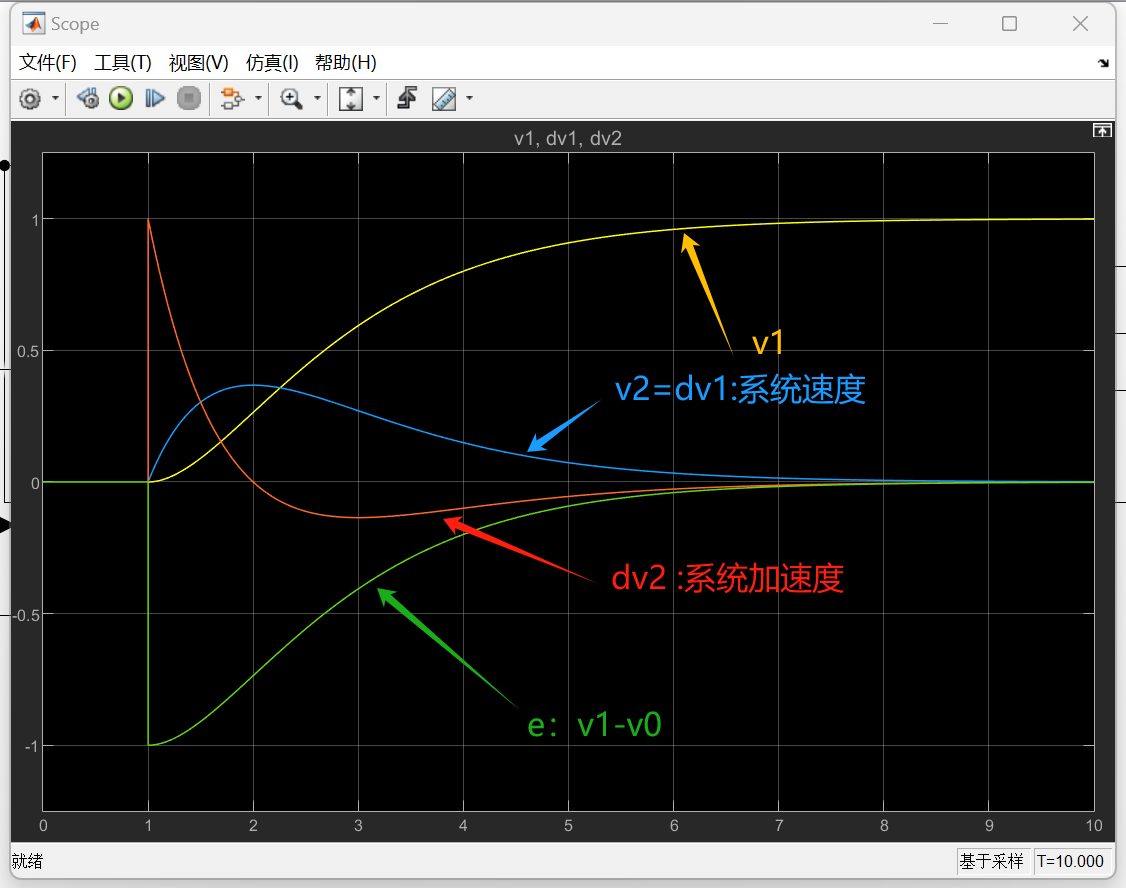
\includegraphics[width=12cm]{picture/tracking_differentiator_scope.png}\\
              通过上图的例子简单地解释一下,当我们的输入为1\ rad时,在0时刻时,误差最大所以角加速度也是最大,随着速度来到了最大值,随着加速度应该反向了,并且让速度减少。\textbf{这样子我们的输入的阶跃信号就变成了$v_1$这个平滑的信号}\\
              从图中我们可以看到,即使误差e一直是负数,系统加速度 $v_2$仍然可能由正变负,这是因为$-k_2v_2$的作用逐渐增强,抑制系统的加速过程, $-k_1e$主导系统的加速或减速趋势,而阻尼项调节加速度的变化速度,二者共同决定了系统的动态行为\\
              \begin{flushleft}
                (2)速度调节\\
              微分信号$v_2$反映跟踪信号的变化速度。通过$-2rv_2$项,系统能够调节过渡过程的速度,避免超调或振荡。\\
              \begin{flushleft}
                这也是我们不用一阶系统的原因,虽然一阶系统一定程度上也可以平滑信号。但是他不存在我们上面所说的对系统靠近目标值的调节。同时我们的跟踪微分器还有一定的滤波作用,这个就让大家matlab自己动手仿真一下了,用matlab看看不同r值的伯德图的样子。

              \end{flushleft}
              \end{flushleft}
              

          \href{https://blog.csdn.net/weiequest_misc=&request_id=&biz_id=102&utm_term=%E8%B7%9F%E8%B8%AA%E5%BE%AE%E5%88%86%E5%99%A8&utm_medium=distribute.pc_search_result.none-task-blog-2~all~sobaiduweb~default-3-124520209.142^v101^pc_search_result_base1&spm=1018.2226.3001.4187}{线性跟踪微分器}


          \subsubsection{代码实现}
          上面讲了这么多,其实跟踪微分器的代码实现并不难,并且我们战队的代码中已经有移植好跟踪微分器了,我们只需要知道怎么去使用就好了
            \par 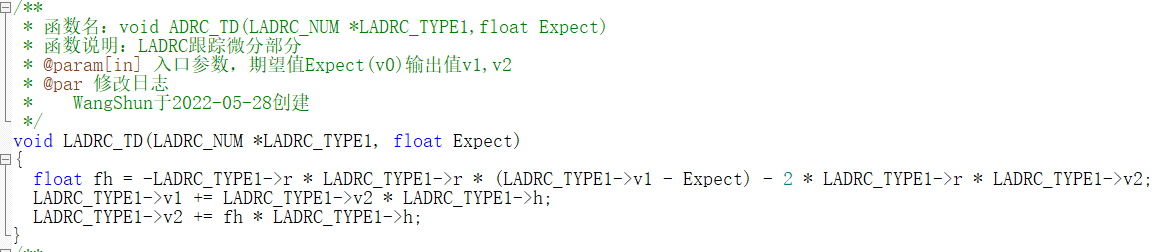
\includegraphics[width=12cm]{picture/tracking_differentiator_code.png}
              \\在ladrc.c中可以找到上面的代码,这和我们上面的状态空间方程是一样的,至于这里为什么要乘一个积分步长,其实这就是采样时间,和我上面写前馈控制器将传递函数化成差分方程是差不多的,但是留意一下这里是将状态空间方程化成差分方程。大致的过程都是差不多的,我这里就不推导了。
            \par 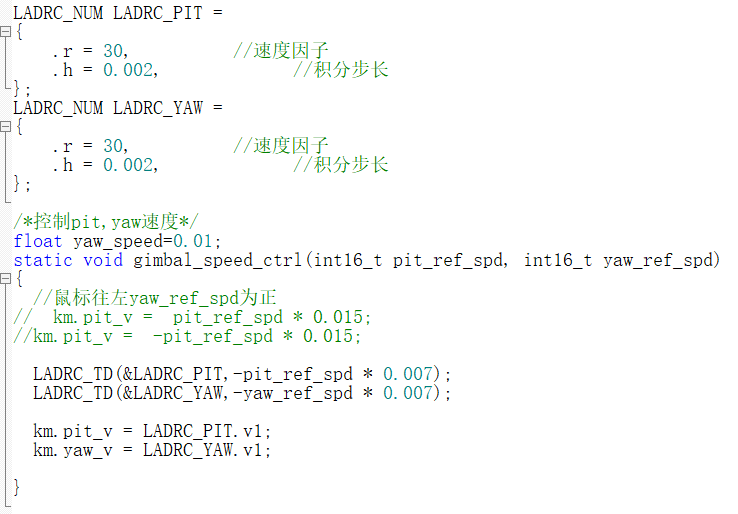
\includegraphics[width=12cm]{picture/tracking_differentiator_code_expng.png}\\
              我们只需要像上面一样定义好结构体的数值,其他的数值可以先不用管,比如观测器输出和观测器带宽等,这需要更多的现控知识,一时之间很难在这份文档里面说完。如果有需要的同学可以自己去研究。\\
              关于r的调参大家只需要根据实际状况去调就好了,毕竟只有一个参数还是很好调的。
              \begin{flushleft}
                在这里我建议看完可以先看\href{https://www.bilibili.com/video/BV1PZ4y1t7DA?spm_id_from=333.788.videopod.episodes&vd_source=b02f21f21dd17ebeef8dac9338c9d06c&p=192}{郭宝龙的信号与系统的工程信号与系统第三章(189—192集)}对状态空间方程有一个大致的概念再去看dr.can的现控。学完现控的知识后,里面说的观测器什么的就自然而然的就理解了。
              \end{flushleft}
              



            \begin{flushleft}
              若有错误的地方可以在github上联系作者和作者讨论。或者说是发QQ邮箱到\textbf{3103942481@qq.com},或谷歌邮箱\textbf{Amos.lab.oss@gmail.com}。出门右转还有一些关于matlab的代码笔记方便大家使用。后面其实还有重力补偿、滤波器、卡尔曼滤波器等知识点因为用的少就没有提及到,有机会的话我还会进行补充,没有机会的话就留给学弟学妹们补充了。
            \end{flushleft}
        \begin{flushright}
          2025.2.18\\
          历时一个月
        \end{flushright}
\end{document}

